% TODO Change language to en_GB (recommended) or en_US for English documents
\documentclass[12pt,a4paper,oneside]{article}             % Single-side
%\documentclass[11pt,a4paper,twoside,openright]{report}  % Duplex

% thanks to http://tex.stackexchange.com/a/47579/71109
\usepackage{ifxetex}
\usepackage{ifluatex}
\newif\ifxetexorluatex % a new conditional starts as false
\ifnum 0\ifxetex 1\fi\ifluatex 1\fi>0
   \xetexorluatextrue
\fi

\ifxetexorluatex
  \usepackage{fontspec}
\else
  \usepackage[T1]{fontenc}
  \usepackage[utf8]{inputenc}
  \usepackage[lighttt]{lmodern}
\fi

\usepackage[english,magyar]{babel} % Alapértelmezés szerint utoljára definiált nyelv lesz aktív, de később külön beállítjuk az aktív nyelvet.

%\usepackage{cmap}
\usepackage{amsfonts,amsmath,amssymb} % Mathematical symbols.
%\usepackage[ruled,boxed,resetcount,linesnumbered]{algorithm2e} % For pseudocodes. % beware: this is not compatible with LuaLaTeX, see http://tex.stackexchange.com/questions/34814/lualatex-and-algorithm2e
\usepackage{booktabs} % For publication quality tables for LaTeX
\usepackage{graphicx}

%\usepackage{fancyhdr}
%\usepackage{lastpage}

\usepackage{anysize}
%\usepackage{sectsty}
\usepackage{setspace} % For setting line spacing

\usepackage[unicode]{hyperref} % For hyperlinks in the generated document.
\usepackage{xcolor}
\usepackage{listings} % For source code snippets.

\usepackage[amsmath,thmmarks]{ntheorem} % Theorem-like environments.

\usepackage[hang]{caption}
\usepackage{subcaption}


%%% MODS COMMENTED

\singlespacing

% \newcommand{\selecthungarian}{
% 	\selectlanguage{magyar}
% 	\setlength{\parindent}{2em}
% 	\setlength{\parskip}{0em}
% 	\frenchspacing
% }
\newcommand{\selecthungarian}{
	\onehalfspacing
	\selectlanguage{magyar}
	\setlength{\parindent}{2em}
	\setlength{\parskip}{0.5em}
	\frenchspacing
}

\newcommand{\selectenglish}{
	\selectlanguage{english}
	\setlength{\parindent}{0em}
	\setlength{\parskip}{0.5em}
	\nonfrenchspacing
	\renewcommand{\figureautorefname}{Figure}
	\renewcommand{\tableautorefname}{Table}
	\renewcommand{\partautorefname}{Part}
	\renewcommand{\chapterautorefname}{Chapter}
	\renewcommand{\sectionautorefname}{Section}
	\renewcommand{\subsectionautorefname}{Section}
	\renewcommand{\subsubsectionautorefname}{Section}
}

\usepackage[numbers]{natbib}
\usepackage{xspace}

% feladatkiíráshoz
\usepackage{pdfpages}


\newcommand{\vikszerzoVezeteknev}{Csarnó}
\newcommand{\vikszerzoKeresztnev}{Tamás Péter}

\newcommand{\vikkonzulensAMegszolitas}{dr.~}
\newcommand{\vikkonzulensAVezeteknev}{Gulyás}
\newcommand{\vikkonzulensAKeresztnev}{Gábor György}

\newcommand{\vikcim}{Gépi tanulási eljárásokkal generált adatok adatvédelmi vizsgálata} % Cím
\newcommand{\viktanszek}{Automatizálási és Alkalmazott Informatikai Tanszék} % Tanszék
\newcommand{\vikdoktipus}{\msc} % Dokumentum típusa (\bsc vagy \msc)
\newcommand{\vikmunkatipusat}{diplomatervet} % a "hallgató nyilatkozat" részhez: szakdolgozatot vagy diplomatervet

\newcommand{\szerzoMeta}{\vikszerzoVezeteknev{} \vikszerzoKeresztnev}

% Beállítások magyar nyelvű dolgozathoz
%--------------------------------------------------------------------------------------
% Elnevezések
%--------------------------------------------------------------------------------------
\newcommand{\bme}{Budapesti Műszaki és Gazdaságtudományi Egyetem}
\newcommand{\vik}{Villamosmérnöki és Informatikai Kar}

\newcommand{\bmemit}{Méréstechnika és Információs Rendszerek Tanszék}

\newcommand{\keszitette}{Készítette}
\newcommand{\konzulens}{Konzulens}

\newcommand{\bsc}{Szakdolgozat}
\newcommand{\msc}{Diplomaterv}
\newcommand{\tdk}{TDK dolgozat}
\newcommand{\bsconlab}{BSc Önálló laboratórium}
\newcommand{\msconlabi}{MSc Önálló laboratórium 1.}
\newcommand{\msconlabii}{MSc Önálló laboratórium 2.}

\newcommand{\pelda}{Példa}
\newcommand{\definicio}{Definíció}
\newcommand{\tetel}{Tétel}

\newcommand{\bevezetes}{Bevezetés}
\newcommand{\koszonetnyilvanitas}{Köszönetnyilvánítás}
\newcommand{\fuggelek}{Függelék}

% Opcionálisan átnevezhető címek
%\addto\captionsmagyar{%
%\renewcommand{\listfigurename}{Saját ábrajegyzék cím}
%\renewcommand{\listtablename}{Saját táblázatjegyzék cím}
%\renewcommand{\bibname}{Saját irodalomjegyzék név}
%}

\newcommand{\szerzo}{\vikszerzoVezeteknev{} \vikszerzoKeresztnev}
\newcommand{\vikkonzulensA}{\vikkonzulensAMegszolitas\vikkonzulensAVezeteknev{} \vikkonzulensAKeresztnev}
\newcommand{\vikkonzulensB}{\vikkonzulensBMegszolitas\vikkonzulensBVezeteknev{} \vikkonzulensBKeresztnev}
\newcommand{\vikkonzulensC}{\vikkonzulensCMegszolitas\vikkonzulensCVezeteknev{} \vikkonzulensCKeresztnev}

\newcommand{\selectthesislanguage}{\selecthungarian}

\bibliographystyle{huplain}

\def\lstlistingname{lista}

\newcommand{\appendixnumber}{6}  % a fofejezet-szamlalo az angol ABC 6. betuje (F) lesz

%--------------------------------------------------------------------------------------
% Page layout setup
%--------------------------------------------------------------------------------------
% we need to redefine the pagestyle plain
% another possibility is to use the body of this command without \fancypagestyle
% and use \pagestyle{fancy} but in that case the special pages
% (like the ToC, the References, and the Chapter pages)remain in plane style

\pagestyle{plain}
\marginsize{35mm}{25mm}{25mm}{25mm}

\setcounter{tocdepth}{3}
%\sectionfont{\large\upshape\bfseries}
\setcounter{secnumdepth}{3}

\sloppy % Margón túllógó sorok tiltása.
\widowpenalty=10000 \clubpenalty=10000 %A fattyú- és árvasorok elkerülése
\def\hyph{-\penalty0\hskip0pt\relax} % Kötőjeles szavak elválasztásának engedélyezése


%--------------------------------------------------------------------------------------
% Setup hyperref package
%--------------------------------------------------------------------------------------
\hypersetup{
    % bookmarks=true,            % show bookmarks bar?
    unicode=true,              % non-Latin characters in Acrobat's bookmarks
    pdftitle={\vikcim},        % title
    pdfauthor={\szerzoMeta},    % author
    pdfsubject={\vikdoktipus}, % subject of the document
    pdfcreator={\szerzoMeta},   % creator of the document
    pdfproducer={},    % producer of the document
    pdfkeywords={},    % list of keywords (separate then by comma)
    pdfnewwindow=true,         % links in new window
    colorlinks=true,           % false: boxed links; true: colored links
    linkcolor=black,           % color of internal links
    citecolor=black,           % color of links to bibliography
    filecolor=black,           % color of file links
    urlcolor=black             % color of external links
}


%--------------------------------------------------------------------------------------
% Set up listings
%--------------------------------------------------------------------------------------
\definecolor{codered}{rgb}{0.82,0.18,0.17}
\definecolor{codegreen}{rgb}{0.5,0.6,0}
\definecolor{codegray}{rgb}{0.5,0.5,0.5}
\definecolor{codepurp}{rgb}{0.75,0.12,0.91}
\definecolor{backcolour}{rgb}{0.97,0.97,0.97}

\definecolor{lightgray}{rgb}{0.95,0.95,0.95}
\lstset{
	basicstyle=\footnotesize\ttfamily, % print whole listing small
	keywordstyle=\color{codered}, % bold black keywords
	identifierstyle=, % nothing happens
	% default behavior: comments in italic, to change use
	commentstyle=\color{codegreen}, % for e.g. green comments
	stringstyle=\color{codepurp},
	showstringspaces=false, % no special string spaces
	aboveskip=9pt,
	belowskip=3pt,
	backgroundcolor=\color{lightgray},
	columns=flexible,
	keepspaces=true,
	escapeinside={(*@}{@*)},
	captionpos=b,
	breaklines=true,
	frame=single,
	float=!ht,
	tabsize=2,
	literate=*
		{á}{{\'a}}1	{é}{{\'e}}1	{í}{{\'i}}1	{ó}{{\'o}}1	{ö}{{\"o}}1	{ő}{{\H{o}}}1	{ú}{{\'u}}1	{ü}{{\"u}}1	{ű}{{\H{u}}}1
		{Á}{{\'A}}1	{É}{{\'E}}1	{Í}{{\'I}}1	{Ó}{{\'O}}1	{Ö}{{\"O}}1	{Ő}{{\H{O}}}1	{Ú}{{\'U}}1	{Ü}{{\"U}}1	{Ű}{{\H{U}}}1
}


%--------------------------------------------------------------------------------------
% Set up theorem-like environments
%--------------------------------------------------------------------------------------
% Using ntheorem package -- see http://www.math.washington.edu/tex-archive/macros/latex/contrib/ntheorem/ntheorem.pdf

\theoremstyle{plain}
\theoremseparator{.}
\newtheorem{example}{\pelda}

\theoremseparator{.}
%\theoremprework{\bigskip\hrule\medskip}
%\theorempostwork{\hrule\bigskip}
\theorembodyfont{\upshape}
\theoremsymbol{{\large \ensuremath{\centerdot}}}
\newtheorem{definition}{\definicio}

\theoremseparator{.}
%\theoremprework{\bigskip\hrule\medskip}
%\theorempostwork{\hrule\bigskip}
\newtheorem{theorem}{\tetel}


%--------------------------------------------------------------------------------------
% Some new commands and declarations
%--------------------------------------------------------------------------------------
\newcommand{\code}[1]{{\upshape\ttfamily\scriptsize\indent #1}}
\newcommand{\doi}[1]{DOI: \href{http://dx.doi.org/\detokenize{#1}}{\raggedright{\texttt{\detokenize{#1}}}}} % A hivatkozások közt így könnyebb DOI-t megadni.

\DeclareMathOperator*{\argmax}{arg\,max}
%\DeclareMathOperator*[1]{\floor}{arg\,max}
\DeclareMathOperator{\sign}{sgn}
\DeclareMathOperator{\rot}{rot}


%--------------------------------------------------------------------------------------
% Setup captions
%--------------------------------------------------------------------------------------
\captionsetup[figure]{
	width=.75\textwidth,
	aboveskip=10pt}

\renewcommand{\captionlabelfont}{\bf}
%\renewcommand{\captionfont}{\footnotesize\it}

%--------------------------------------------------------------------------------------
% Hyphenation exceptions
%--------------------------------------------------------------------------------------
\hyphenation{Shakes-peare Mar-seilles ár-víz-tű-rő tü-kör-fú-ró-gép}


\author{\vikszerzo}
\title{\viktitle}


%--------------------------------------------------------------------------------------
% Table of contents and the main text
%--------------------------------------------------------------------------------------
\begin{document}

\pagenumbering{roman}
\selectthesislanguage

% Feladatkiírás
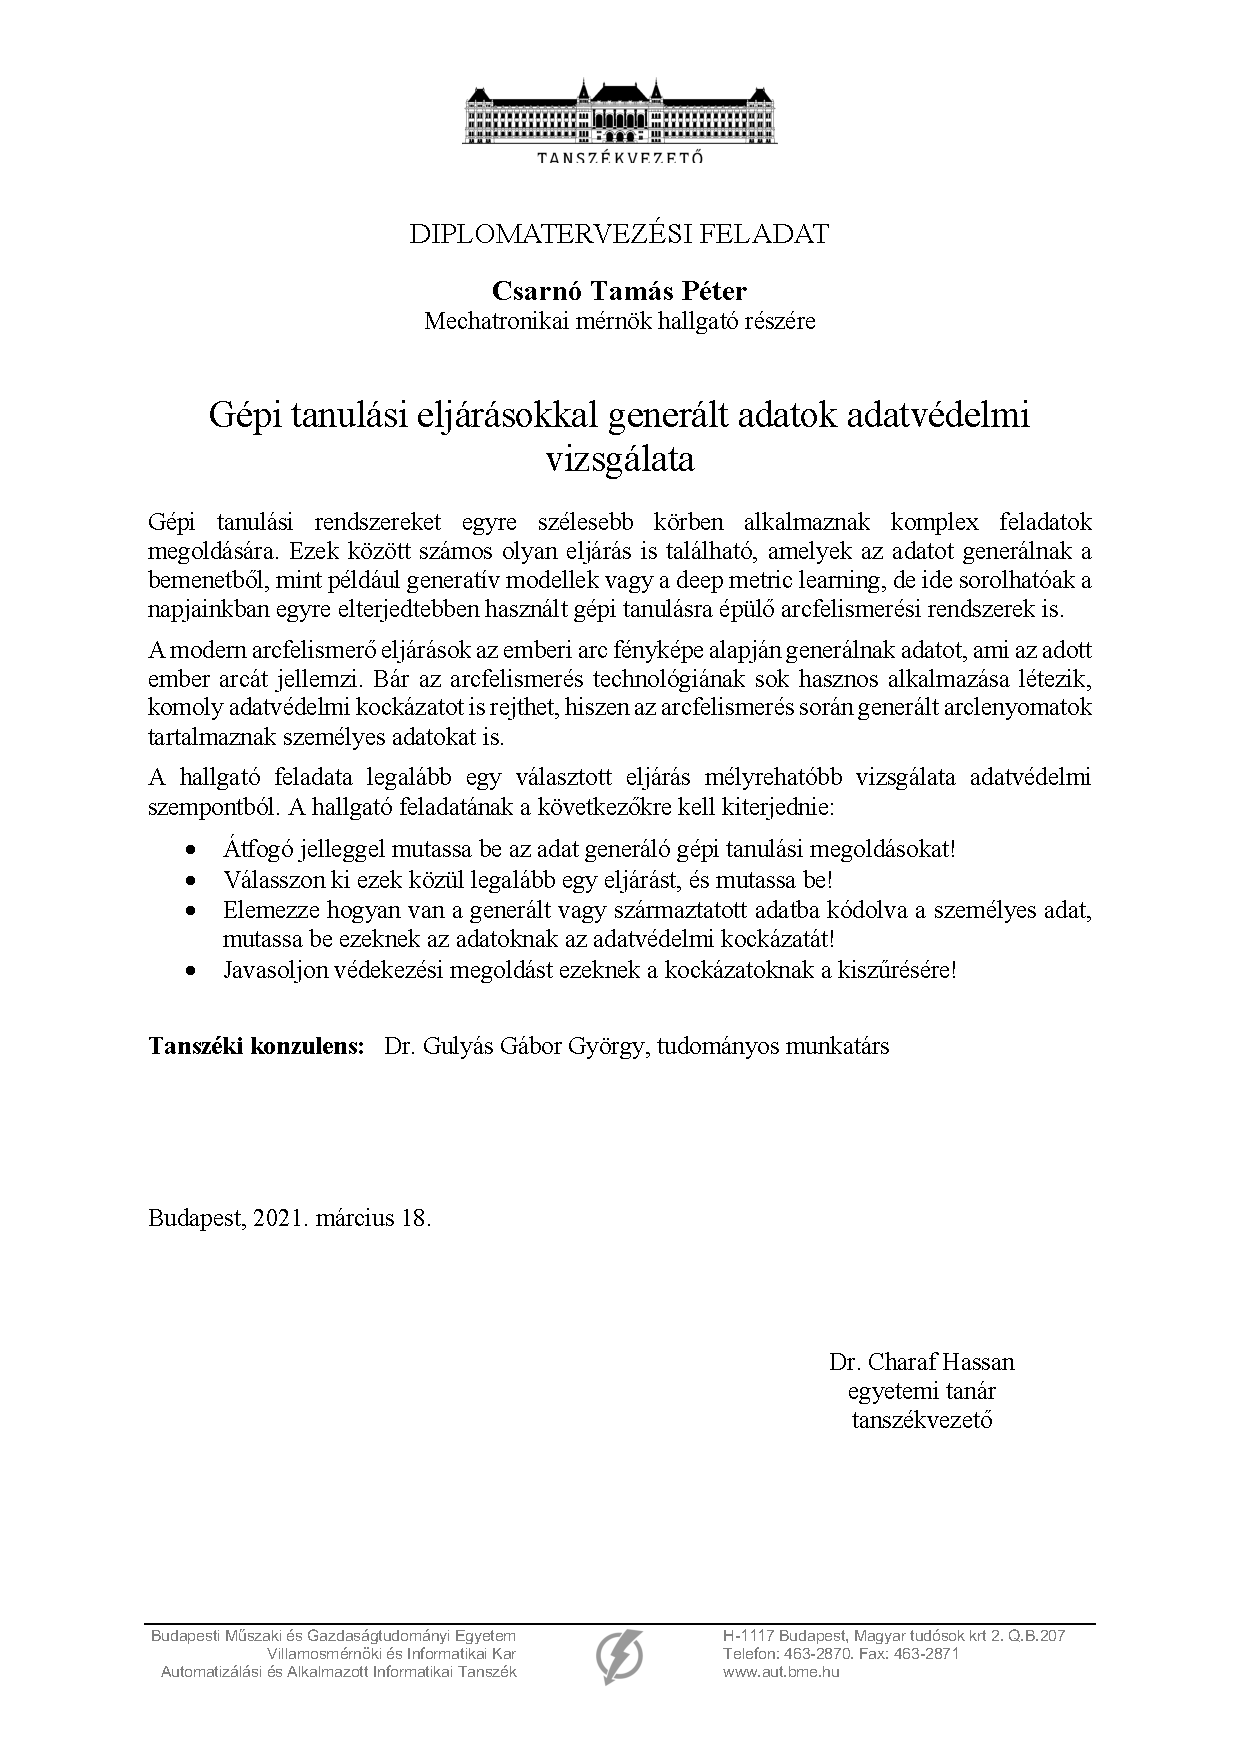
\includepdf[pages=-]{include/feladatkiiras.pdf}

% Titlepage
%~~~~~~~~~~~~~~~~~~~~~~~~~~~~~~~~~~~~~~~~~~~~~~~~~~~~~~~~~~~~~~~~~~~~~~~~~~~~~~~~~~~~~~
\hypersetup{pageanchor=false}
%--------------------------------------------------------------------------------------
%	The title page
%--------------------------------------------------------------------------------------
\begin{titlepage}
\begin{center}

\includegraphics[width=60mm,keepaspectratio]{figures/bme_logo.pdf}\\
\vspace{0.3cm}
\textbf{\bme}\\
\textmd{\vik}\\
\textmd{\viktanszek}\\[5cm]

\vspace{0.4cm}
{\huge \bfseries \vikcim}\\[0.8cm]
\vspace{0.5cm}
\textsc{\Large \vikdoktipus}\\[4cm]

{
	\renewcommand{\arraystretch}{0.85}
	\begin{tabular}{cc}
	 \makebox[7cm]{\emph{\keszitette}} & \makebox[7cm]{\emph{\konzulens}} \\ \noalign{\smallskip}
	 \makebox[7cm]{\szerzo} & \makebox[7cm]{\vikkonzulensA} \\
	%   & \makebox[7cm]{\vikkonzulensB} \\
	\end{tabular}
}

\vfill
{\large \today}
\end{center}
\end{titlepage}
\hypersetup{pageanchor=false}

		   % Szakdolgozat/Diplomaterv címlap

% Table of Contents
%~~~~~~~~~~~~~~~~~~~~~~~~~~~~~~~~~~~~~~~~~~~~~~~~~~~~~~~~~~~~~~~~~~~~~~~~~~~~~~~~~~~~~~
\tableofcontents\vfill

% Declaration and Abstract
%~~~~~~~~~~~~~~~~~~~~~~~~~~~~~~~~~~~~~~~~~~~~~~~~~~~~~~~~~~~~~~~~~~~~~~~~~~~~~~~~~~~~~~
% \selectlanguage{magyar}
\pagenumbering{gobble}
%--------------------------------------------------------------------------------------
% Nyilatkozat
%--------------------------------------------------------------------------------------
\begin{center}
\large
\textbf{HALLGATÓI NYILATKOZAT}\\
\end{center}

Alulírott \emph{\vikszerzoVezeteknev{} \vikszerzoKeresztnev}, szigorló hallgató kijelentem, hogy ezt a \vikmunkatipusat{} meg nem engedett segítség nélkül, saját magam készítettem, csak a megadott forrásokat (szakirodalom, eszközök stb.) használtam fel. Minden olyan részt, melyet szó szerint, vagy azonos értelemben, de átfogalmazva más forrásból átvettem, egyértelműen, a forrás megadásával megjelöltem.

Hozzájárulok, hogy a jelen munkám alapadatait (szerző(k), cím, angol és magyar nyelvű tartalmi kivonat, készítés éve, konzulens(ek) neve) a BME VIK nyilvánosan hozzáférhető elektronikus formában, a munka teljes szövegét pedig az egyetem belső hálózatán keresztül (vagy autentikált felhasználók számára) közzétegye. Kijelentem, hogy a benyújtott munka és annak elektronikus verziója megegyezik. Dékáni engedéllyel titkosított diplomatervek esetén a dolgozat szövege csak 3 év eltelte után válik hozzáférhetővé.

\begin{flushleft}
\vspace*{1cm}
Budapest, \today
\end{flushleft}

\begin{flushright}
 \vspace*{1cm}
 \makebox[7cm]{\rule{6cm}{.4pt}}\\
 \makebox[7cm]{\emph{\vikszerzoVezeteknev{} \vikszerzoKeresztnev}}\\
 \makebox[7cm]{hallgató}
\end{flushright}
\thispagestyle{empty}

\vfill
% \clearpage
% \thispagestyle{empty} % an empty page

\selectthesislanguage
 %TODO Hallgatói nyilatkozat
% \pagenumbering{roman}
\setcounter{page}{1}
\selecthungarian

%----------------------------------------------------------------------------
% Abstract in Hungarian
%----------------------------------------------------------------------------
\section*{Kivonat}\addcontentsline{toc}{section}{Kivonat}

Magyar rész.


\newpage
\selectenglish
%----------------------------------------------------------------------------
% Abstract in English
%----------------------------------------------------------------------------
\section*{Abstract}\addcontentsline{toc}{section}{Abstract}

English part.


\vfill
\selectthesislanguage




% The main part of the thesis
%~~~~~~~~~~~~~~~~~~~~~~~~~~~~~~~~~~~~~~~~~~~~~~~~~~~~~~~~~~~~~~~~~~~~~~~~~~~~~~~~~~~~~~
\pagenumbering{arabic}
%----------------------------------------------------------------------------
\section{\bevezetes}
%----------------------------------------------------------------------------

%--------------------------------
% advancement in ML, GPUs, big data

Az elmúlt években a nagyméretű adathalmazok elérhetőségének, a számítási kapacitás exponenciális növekedésének és a mély tanulás területén elért áttöréseknek köszönhetően jelentősen megnövekedett az érdeklődés a gépi tanulás iránt. Manapság a gépi tanulási algoritmusokat előszeretettel alkalmazzák nagy dimenziós bemeneti adatokhoz kapcsolódó osztályozási, regressziós, klaszterezési vagy dimenziócsökkentési feladatokra. A gépi tanulási algoritmusok számos területen embert meghaladó képességekkel rendelkeznek (például képosztályozásban). A mindennapi életünkben használt okos eszközökön a kép- és beszédfelismerést, az internetes keresést, az arcfelismeréses bejelentkezést, stb. a gépi tanulási algoritmusok tesznek lehetővé.

% In recent years, the availability of large datasets combined with the improvement in algorithms and the exponential growth in computing power led to an unparalleled surge of interest in the topic of machine learning. Nowadays, machine learning algorithms are successfully employed for classification, regression, clustering, or dimensionality reduction tasks of large sets of especially high-dimensional input data.1 In fact, machine learning has proved to have superhuman abilities in numerous fields (such as playing go,2 self driving cars,3 image classification,4 etc). As a result, huge parts of our daily life, for example, image and speech recognition,5,6 web-searches,7 fraud detection,8 email/spam filtering,9 credit scores,10 and many more are powered by machine learning algorithms.

A gépi tanulás nagy részben hozzájárult a tudomány és technológia fejlődéshez. Szinte minden iparág és vállalat felismerte a gépi tanulás előnyeit és lehetőségeit. A technológia fejlődése lehetővé tette a közelmúltbeli áttöréseket, amelyek elősegítik a gyorsabb és hatékonyabb üzleti intelligenciát, az arcfelismeréstől a természetes nyelvfeldolgozásig terjedő alkalmazások felhasználásával.

% Advances in this technology have allowed for recent breakthroughs that promote faster and more efficient business intelligence, using abilities ranging from facial recognition to natural language processing.

% ml -> fejlődés
% áttörések, pl arcfelismerés, nlp
%  ???
% alkalmazások között van ami generálni tud adatot a bemenetből
% 

% --------------------------------
% adatgeneráló eljárások megjelenése, motivációja (moar data)

A gépi tanulás alkalmazásai között szerepelnek olyan eljárások, amelyek képesek adatot generálni a bemenetből, mint például a generatív modellek vagy a mély metrika tanulás, de ide sorolhatóak a napjainkban egyre elterjedtebben használt gépi tanulásra épülő arcfelismerési rendszerek is.

% ide példa...
% példa lehet
% egy GAN példa ide -> 

A generatív modellek egyik típusa: a GAN (Generative Adversarial Network) olyan neurális hálózatok, amelyek képesek új, szintetikus adatot előállítani. A GAN egy olyan neurális háló, amelyben két alhálózat verseng egymással: a generátor és a diszkriminátor. A generátor feladata a tanító mintákhoz hasonló új minták előállítása, míg a diszkriminátor felel a valódi és a generált minták megkülönböztetéséért. A GAN tanítása során a generátor igyekszik egyre hihetőbb mintákat előállítani, hogy be tudja csapni a diszkriminátort. A GAN-ok sikeres betanítása után, a bemenetre adott véletlenszerű zajból realisztikus képeket tudnak generálni. Például az NVIDIA által fejlesztett StyleGAN3 képes fotorealisztikus emberi arcok generálására \cite{stylegan3}.

A GAN-ok elsősorban olyan szituációkban lehetnek nagyon hasznosak, amikor több tanítóadatra van szükségünk, viszont az adat gyűjtése nehezen megoldható. Sok esetben az adatgyűjtés és címkézés hosszadalmas, drága folyamat. Amennyiben be tudunk tanítani egy hálót, ami a célnak megfelelő minőségű szintetikus adatok előállítására képes, az megoldást adhat erre a problémára. Az új adatoknak megfelelően realisztikusnak kell lenniük ahhoz, hogy a generált adatokból szerzett ismeretek továbbra is érvényesek legyenek a valós adatokra. 

% CUT
% A generatív modellek leírják egy adathalmaz előállításának módját a valószínűségi modell alapján. Ebből a modellből mintavételezéssel új adatokat tudunk előállítani. A GAN -ok olyan struktúrát fedeznek fel az adatokban, amely lehetővé teszi számukra, hogy reális adatokat állítsanak elő.

% A GAN egy generatív modell, amelyben két neurális háló verseng egymással.  Az első hálót generátornak nevezik. A generátor felelős új szintetikus minták előál- lításáért, amelyek hasonlítanak a tanító halmaz mintáihoz. A másik neurális hálót diszkriminátornak nevezik, aminek a feladata megkülönböztetni a valódi minták (tanító minta) illetve a generátor által létrehozott szintetikus minták között. A ge- nerátor célja becsapnia a diszkriminátort, míg a diszkriminátor megpróbál ennek ellenállni. A két háló versengéséből ered az „adversarial” elnevezés.

% GAN is a type of neural network that is able to generate new data from scratch. You can feed it a little bit of random noise as input, and it can produce realistic images of bedrooms, or birds, or whatever it is trained to generate. One thing all scientists can agree on is that we need more data. GANs, which can be used to produce new data in data-limited situations, can prove to be really useful. Data can sometimes be difficult and expensive and time-consuming to generate. To be useful, though, the new data has to be realistic enough that whatever insights we obtain from the generated data still applies to real data. If you’re training a cat to hunt mice, and you’re using fake mice, you’d better make sure that the fake mice actually look like mice.


% A generative model can be broadly defined as follows: A generative model describes how a dataset is generated, in terms of a probabilistic model. By sampling from this model, we are able to generate new data. Another way of thinking about it is the GANs are discovering structure in the data that allows them to make realistic data. This can be useful if we can’t see that structure on our own or can’t pull it out with other methods. 

% A mélygenerációs modellek (DGM) alkalmazásai, mint például a híres képekből hamis portrék készítése, nemrégiben címlapokra kerültek. Ezen úgynevezett mély hamisítványok megjelenése jelentős társadalmi és jogi kihívások elé állít, de új előnyös technológiákat is ígér.

% Applications of deep generative models (DGM), such as creating fake portraits from celebrity images, have recently made headlines. The advent of these so-called deep fakes poses considerable societal and legal challenges, but also promise new beneficial technologies [10].

% --------------------------------
% arcfelismerés -> egyre több kamera

A gépi tanulási technikák fejlődésének köszönhetően, illetve az egyre olcsóbb okos eszközök elterjedésével, egyre jobban elterjedt az arcfelismerés használata. A generatív modellekhez hasonlóan, a modern arcfelismerő rendszerek is gépi tanulásra támaszkodnak. Működésük során az emberek arcáról készült digitális képekből képesek arcot jellemző metrikákat előállítani oly módon, hogy egy emberhez tartozó arcleíró vektorok (későbbiekben arclenyomatok) távolsága kicsi legyen, míg különböző emberek között minél nagyobb. Erre a célra létrehozott neurális hálók: a sziámi hálók képesek megtanulni azt a mély metrikát, ami legjobban leírja az emberi arc struktúráját. Miután sikerült betanítani egy hálót ami képes digitális arcképekből arclenyomatokat származtatni, az arclenyomatok összehasonlításával már képes a rendszer összevetni a keresett személyt a rendszer által ismert személyekkel.

% arcfelismerés és adatvédelem -> arclenyomatvektor

Az ilyen módon kinyert arclenyomatokban tárolt információ ember számára nem értelmezhető, csupán egy lebegőpontos számsornak tűnik, de belőlük gépi tanulási módszerekkel személyes adat származtatható a képen látható személyekről. Magukba kódolva olyan információkat is hordoznak, mint például a képen látható illető rassza, a neme, életkora és az arc egyéb jellemzői. Ezek az információk együttesen lehetővé teszik egy személy azonosítását. Az arclenyomatokban hordozott információk alapján lehetséges az eredeti arcképek rekonstruálása \cite{mai2018reconstruction}. Az így kapott arcképek kevésbé részletgazdagok, mint az eredeti.

%CUT itt lehet vágni egyet


% While these seem as a list of arbitrary numbers to the naked eye, they may contain personal information about the person whose photo was taken. In their recent work, Mai et al. showed that the photo itself can be reconstructible from the embedding. In authors argue that it should be an accepted fact that with good accuracy the original sample can be reconstructed from unprotected embeddings. This means that sensitive data could be derived from unprotected templates and other attacks can also be launched based on the reconstruction results. Based on this, it can also be possible to reverse engineer data from face embeddings in order to find out the original identity of the embedding

% cél

A dolgozatomban azt vizsgálom, hogy a gépi tanulás alapú arcfelismerés által kinyert arclenyomatok lehetővé teszik-e az arclenyomat forrását, az eredeti alanynak a felismerését. Megvizsgálom, hogy az arclenyomatok hogyan kódolják az arc struktúráját, illetve, hogy annak mely részei hordoznak érzékeny információt az adatalanyról. Célom arclenyomatok vizsgálatát olyan módszerrel végezni, amely általánosítható lehet akár generatív modelleknél használt belső reprezentációk analízisére.

A dolgozatom felépítése a következő. A \ref{sec:irodalom}. fejezetben a témámhoz kapcsolódó fontosabb témaköröket mutatom be, amit a \ref{sec:problem}. fejezetben a probléma bemutatása követ. A \ref{sec:4}. fejezetben az arclenyomatokhoz kapcsolódó adatvédelmi kérdésekkel foglalkozom. Az \ref{sec:5}. fejezetben azt vizsgálom, milyen információkat hordozhat egy arclenyomat, azok miként manipulálhatóak. A \ref{sec:6}. fejezetben javaslatot teszek az adatvédelmi kockázatok kezelésére.

% Ezért munkám során az elmúlt időszakban azt vizsgáltam, hogy a gépi tanulás alapú arcfelismerés által kinyert ún. embeddingek, lehetővé teszik-e az embedding forrását, az eredeti adatalanynak a felismerését, és ha igen, akkor mely részei kódolják az egyes információkat. A célom, hogy meghatározzam az arclenyomat vektorok (embeddingek) azon koordinátáit, amelyek az érzékeny információkat hordozzák, például a rasszt. Ezt különböző gépi tanulás elemzésére és értelmezésére használható eszközökkel hajtom végre. Az itt meghatározott koordinátákat módosítjuk vagy töröljük. Ezek után vizsgáljuk, hogy ennek hatására hogyan változik az érzékeny információ meghatározására alkalmas modellek pontossága.

% We live in times when efficient uses of artificial intelligence and cheap smart technology are exploding. By the spread of smart cameras, applications on facial recognition had become almost ubiquitous in some cities around the world. In some cases we can find the driver reason for this in the security concerns of the public, but face recognition (or FR in short) can be applied to a much broader set of use-cases. Beside identification or authentication of individuals in crowds, it could benefit the society also in criminal detection, searching for lost people, customer behavior analysis, etc.

% However, FR technology could be abused and therefore it has the potential to pose risks to individuals, to the society and even to the governmental and business sectors, as well. This puts related ethical issues into the focus.

% The 2010s kickstarted the modern era of facial recognition, as computers were finally powerful enough to train the neural networks required to make facial recognition a standard feature.
% Facial recognition first trickled into personal devices as a security feature with Windows Hello and Android’s Trusted Face in 2015, and then with the introduction of the iPhone X and Face ID in 2017.

% Proponents of facial recognition suggest that the software is useful because alongside identifying suspects, it can monitor known criminals and help identify child victims of abuse. In crowds, it could monitor for suspects at large events and increase security at airports or border crossings. The most long-running type of facial recognition software runs a photo through a government-controlled database, such as the FBI’s database of over 400 million photos, which includes driver’s licenses from some states, to identify a suspect. Local police departments use a variety of facial recognition software, often purchased from private companies.

% There’s a long list of benefits facial recognition can offer outside of law enforcement, adding convenience or security to everyday things and experiences. Facial recognition is helpful for organizing photos, useful in securing devices like laptops and phones, and beneficial in assisting blind and low-vision communities. It can be a more secure option for entry into places of business, fraud protection at ATMs, event registration, or logging in to online accounts. Advertising and commercial applications of facial recognition promise a wide array of supposed benefits, including tracking customer behavior in a store to personalize ads online.

% Face recognition systems are being increasingly used for secure access in applications ranging from personal devices to access control (e.g., banking and border control). In critical applications, face recognition needs to meet stringent performance requirements, including low error rates and strong system security. In particular, the face recognition system must be resistant to spoofing (presentation) attacks and template invertivility. Therefore, it is critical to evaluate the vulnerabilities of a face recognition system to these attacks and devise necessary countermeasures. To this end, several attack mechanisms (such as hill climbing [1], [2], [3], spoofing [4], [5], [6], [7], [8], and template reconstruction (template invertibility) [9]) have been proposed to determine the vulnerabilities of face recognition systems.

% A 2. chapterben ... a 3. chapterben ... a 4. chapterben ...
%----------------------------------------------------------------------------
\section{Irodalomkutatás}
\label{sec:irodalom}
%----------------------------------------------------------------------------

% \subsection{Generatív modellek csoportosítása}

% \subsubsection{Supervised learning}

A gépi tanulási modellek csoportosíthatók a feladat típusa alapján: megkülönböztetünk felügyelt és felügyelet nélküli, illetve megerősítéses tanulást.

\begin{figure}[h]
	\centering
	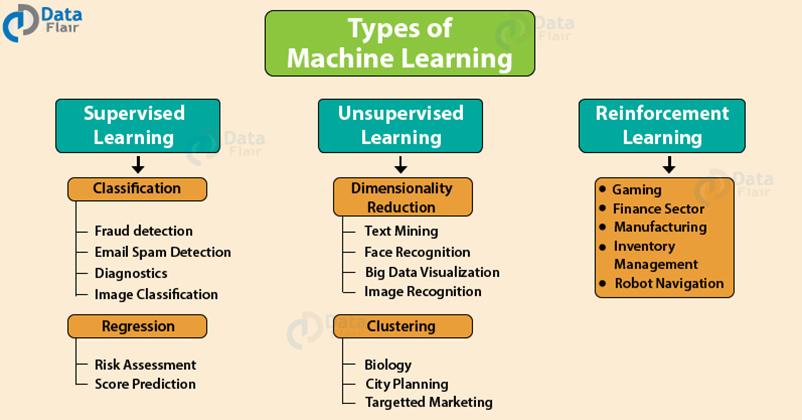
\includegraphics[width=1\columnwidth]{figures/machine_learning_types.png}
	\caption{Gépi tanulás csoportosítása}
\end{figure}

% TODO ezt újraírni, mert katyvasz
A felügyelt tanulásról akkor beszélünk, amikor ismerjük a tanító mintakészlethez tartozó elvárt kimeneteket. Az ilyen mintakészletet címkézettnek nevezzük. A felügyelt tanulás célja egy olyan funkció elsajátítása, amely az adatok mintázata és a címkék alapján a legjobban közelíti a bemenet és kimenet közötti kapcsolatot. Az ilyen modelleket címkézett adatokon tanítanak be, majd a modell által korábban nem látott új mintákra képest helyes becslést adni. A felügyelt tanulásnak két alkategóriája van, a regresszió és az osztályozás vagy más nével klasszifikáció. Osztályozás esetén a kimenetet két vagy több osztályba kell csoportosítani. Ha az algoritmus a bemenetet két különböző osztályba sorolja, akkor ezt bináris osztályozásnak nevezzük, míg a több mint két osztály közötti választást többosztályos osztályozásnak nevezzük. Ezzel szemben a regressziós algoritmusokat folytonos értékek előrejelzésére használják, mint például az ár, a fizetés és az életkor. 

A felügyelet nélküli tanulás esetén a megfigyelésekhez nem áll rendelkezésre elvárt célérték (azaz felügyelet). Célunk, hogy az adatok belső mintázatait, összefüggéseit azonosítsunk. A tanítás itt a kérdéses mintázat/összefüggés definícióját jelenti, ami általában számos mérnöki iteráció után alakul ki. felügyelet nélküli tanulást alkalmaznak többek között klaszterezési feladatok megoldására, dimenziócsökkentésre, asszociációs feladatokra, anomália detektálásra, illetve generatív modellekhez is \cite{ghahramani2003unsupervised}.

% In Supervised Learning, we train the machine using data that is well “labeled”. It means the data is already tagged with the correct answer. A supervised learning algorithm learns from labeled training data and predicts outcomes for unforeseen data. There are two subcategories of supervised learning, Regression and Classification. Classification means to group the output into a class. If the algorithm tries to label input into two distinct classes, it is called binary classification. Selecting between more than two classes is referred to as multiclass classification. On the other hand, Regression Algorithms are used to predict continuous values such as price, salary, and age.

%--------------
% Felügyelt tanulás (supervised learning): a tapasztalatok itt egy megfigyelés/adat és a hozzá tartozó elvárt célérték. A tapasztalatok halmaza egyben adott, ezt hívjuk tanító adatbázisnak (training dataset). A cél, hogy ez alapján olyan modellt tanuljunk ami korábban nem látott példákon is helyesen működik. Példa alkalmazás: ügyfélszolgálatra érkező e-mail panaszleveleket akarunk automatikusan továbbítani a megfelelő munkatárshoz, aki meg tudja válaszolni azt. Ehhez rendelkezésre áll több ezer e-mail a múltból (adat) és, hogy melyik munkatárshoz kellett irányítani a levelet (elvárt célérték). Ebből a tanító adatbázisból kell megtanulnunk egy modellt, ami a holnap érkező e-maileket a lehető legnagyobb pontossággal automatikusan a megfelelő munkatárshoz irányítja.  
% Felügyelet nélküli tanulás (unsupervised learning): A megfigyelésekhez nem áll rendelkezésre elvárt célérték (azaz felügyelet). Célunk, hogy az adatok közt mintázatokat/összefüggéseket azonosítsunk. A tanítás itt a kérdéses mintázat/összefüggés definícióját jelenti, ami általában számos mérnöki iteráció után alakul ki.  Példa alkalmazás: a vállalat ügyfeleiről rendelkezésre állnak azok múltbeli tranzakcióinak adatai. Találjunk olyan ügyfél csoportokat, akik hasonlóan viselkednek anélkül, hogy a viselkedési csoportokat előre megadnánk! Figyelem, mérnöki feladat, hogy két tranzakciósorozat hasonlóságt leírjuk!  
% Megerősítéses tanulás (reinforcement learning): a rendszer folyamatosan akciókat hajt végre, néha kap megerősítést, hogy mennyire jól csinálja a feladatát, és ezekből a megerősítésekbő folyamatosan tanul.  Példa alkalmazás: Robotot tanítunk büntetőt rúgni fociban. A robot csak a büntetőrúgás végén kap visszajelzést, hogy sikeres volt-e. Ebből kell saját magának kialakítani a mozgássorozatot, amire majd megint kap megerősítést (aktív tanulás).
%-------------- (https://www.inf.u-szeged.hu/~rfarkas/ML20/alapfogalmak.html)

% Unsupervised Learning is a machine learning technique, where the model does not need any supervision. Instead, we need to allow the model to work on its own to discover information. It mainly deals with the unlabelled data. Density estimation, dimensionality reduction, and clustering and some of the main applications of unsupervised learning.

% In Machine learning, supervised learning methods are used when the objective is to learn mapping between the attributes and the target in the data. When the objective is to identify the underlying structure or the pattern in the data, unsupervised learning methods are useful. Some of the popular unsupervised learning methods are Clustering, Dimensionality reduction, Association mining, Anomaly detection and Generative models. Each of these techniques have a different pattern recognition objective such as identifying latent grouping, identifying latent space, finding irregularities in the data, density estimation or generating new samples from the data. 

%----------------------------------------------------------------------------
% \subsubsection{Generative vs discriminative modeling}

A gépi tanulási modelleket feladatuk szerint két további alkategóriába sorolhatjuk: generatív és diszkriminatív modellek. 

\begin{figure}[h]
	\centering
	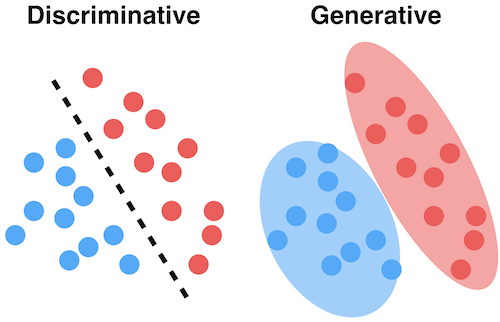
\includegraphics[width=0.65\columnwidth]{figures/generative_discriminative.png}
	\caption{Diszkriminatív és generatív modellek közötti eltérés. (forrás: \cite{fig:generative_discriminative})}
\end{figure}

% TODO újraírni, lényeg legyen benne
A diszkriminatív modellek a statisztikai osztályozásban használt modellek egy osztályába tartoznak. Ezeket főként felügyelt gépi tanulási feladatokra használnak. Az ilyen típusú modelleket feltételes modelleknek is nevezik, mivel megtanulják az osztályok vagy címkék elhatárolását egy adathalmazban. A diszkriminatív modellek (akárcsak a szó szerinti értelemben) a feltételes valószínűség modellezése helyett elkülönítik az osztályokat, és nem tesznek feltételezéseket az adatpontokról. Ezek a modellek azonban nem képesek új adatpontok előállítására. Ezért a diszkriminatív modellek végső célja az egyes osztályok elkülönítése egymástól.

%----------
A generatív modellek a felügyelet nélküli tanulásban használatosak. Ezek a modellek képesek megtanulni a tanító minták valószínűségi eloszlását, majd tanítás után új minták generálására képesek. Ez a tulajdonság a gyakorlatban rendkívűl előnyös. A mély tanulásban használt modellek betanításához nagy mennyiségű, és megflelelő minőségű adatra van szükség, ezért az ezzel foglalkozó vállalatok rengeteg erőforrást áldoznak a tanítóminták begyűjtésére. Jellemzően manuális annotációra van szükség ami munkaigényes folyamat. Ez a megközelítés költséges, és nehezen skálázható. A jó minőségű adathoz tipikusan csak a nagyobb vállalatok képesek hozzájutni. A generatív modellek használatával több válalat képes minőségi tanítóadatot előállítani lényegesen kevesebb mintából.

% ezt lehetne szövegesen kifejteni mert érdekes.
A generatív modelleknek számos érdekes felhasználási területe van, ezek közül néhány példa:
\begin{itemize} 
	\item Fotorealisztikus emberi arcképek generálására képes \cite{stylegan3}.
	\item Egy képet leíró szöveg alapján képes képet készíteni \cite{reed2016generative}.
	\item Az adathalmazban ritkán előforduló adatok generálását tudja, ami kiegyensúlyozhatja az adatot.
	\item Realisztikusan képes utánozni az emberi hangot \cite{jia2018transfer}.
\end{itemize}

% ~~~
% The learning models in machine learning can be classified into two sub-categories, Discriminative models and Generative models. Discriminative models classify input data; i.e., given the features of an instance of data, they predict a label or category to which that data belongs. In Supervised Learning, the classification algorithms/models are examples of discriminative models.

% Generative Modelling is an unsupervised learning task in machine learning that involves generating new data samples from the probability distribution of training data. Given some data, the aim is to have a model for the underlying probability distribution of that data so that we can draw samples that are similar to our training data.

%~~~~~~~~~~
% Machine learning models can be classified into two types of models – Discriminative and Generative models. In simple words, a discriminative model makes predictions on the unseen data based on conditional probability and can be used either for classification or regression problem statements. On the contrary, a generative model focuses on the distribution of a dataset to return a probability for a given example.
%~~~~~~~~~~ (https://www.analyticsvidhya.com/blog/2021/07/deep-understanding-of-discriminative-and-generative-models-in-machine-learning/)

%~~~~~~~~~
A generatív modellek megértéséhez vegyünk egy példát. Tegyük fel, hogy van egy adathalmazunk, amely emberi arcokról készült fényképeket tartalamz. Egy olyan gépi tanulási modellt szeretnénk betanítani az adathalmazunk alapján, amely képes egy nem létező emberekről valóságosnak tűnő arcképet generálni. Egy ilyen feladat megoldható generatív modellezéssel. A \ref{fig:generative_model}. ábra egy tipikus generatív modellezési folyamatot mutat be.

\begin{figure}[h]
	\centering
	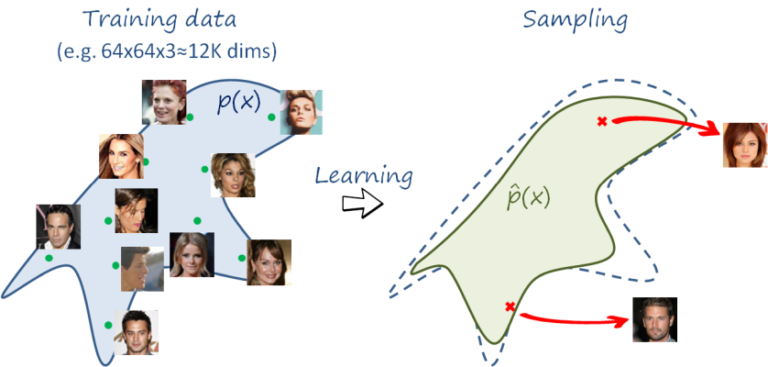
\includegraphics[width=0.9\columnwidth]{figures/generative_model_struct.png}
	\caption{A betanított generatív modell által megtanul eloszlás $\hat{p}(x)$ jól közelíti a valódi adateloszlást $p(x)$. (forrás: \cite{fig:generative_model_struct})}
	\label{fig:generative_model}
\end{figure}

Először is szükségünk van egy adathalmazra, amely számos mintát tartalmaz az általunk generálni kivánt dologról. Az adathalmaz egyes elemeit megfigyeléseknek (observation) is nevezik. Minden megfigyelés sok jellemzőből (feature) áll amelyek képek esetén az egyes pixelek értékeit jelentik. Célunk egy olyan modell létrehozása, amely képes olyan új megfigyeléseket generálni, amelyek jellemzői jól közelítik az eredeti adathalmazban lévő jellemzőket. Képgenerálás esetén ez egy rendkívűl nehéz feladat, mivel az egyes pixelek rengeteg lehetséges értéket vehetnek fel, és ezek közül csak relatíve kevés konfiguráció felel meg annak a képnek amit mi generálni szeretnénk.

A generatív modellek sztochasztikus jellegűnek kell lennnie, nem pedig determinisztikusnak. Ha a modellünk csupán egy fixált számítást végezne, példáuk az adathalmaz minden egyes pixelének átlagát számolná, akkor a modell minden alkalommal ugyanazt a kimenetet eredményezi. Így a generatív modellek szükségszerűen tartalmaznia kell egy véletlenszerű elemet, amely befolyásolja a modell által generált mintákat.

Más szavakkal, létezik egy ismeretlen valószínűségi eloszlás, amely leírja, hogy az egyes képek miért találhatóak a mintakészletünkban, míg más képek nem. A gyakorlatban nem ismerjük a tényleges valószínűségi eloszlást, ezért azt csak közelíteni tudjuk a megfigyelésekből. A generatív modellek célja az, hogy ezt az ismeretlen eloszlást minél jobban közelítse. A modell tanítása után a  megtanult eloszlást mintavételezve olyan megfigyeléseket kaphatunk, amelyek az eredeti adathalmaz elemeihez nagyon hasonlóak.

%------------
% In practice, we may not be able to assess or observe all possible outcomes of a random variable due to which we generally do not know the actual density function. In such conditions, we must rely on approximating the density function from a sample of observations. Approximating a density function using a sample of observations is referred to as ‘Density estimation’.  Learning density estimate from the training samples is fundamental to generative models.
%~~~~~~~~~~~
% Suppose we have a dataset containing images of horses. We may wish to build a model that can generate a new image of a horse that has never existed but still looks real because the model has learned the general rules that govern the appearance of a horse. This is the kind of problem that can be solved using generative modeling. A summary of a typical generative modeling process is shown in Figure 1-1.

% First, we require a dataset consisting of many examples of the entity we are trying to generate. This is known as the training data, and one such data point is called an observation. Each observation consists of many features—for an image generation problem, the features are usually the individual pixel values. It is our goal to build a model that can generate new sets of features that look as if they have been created using the same rules as the original data. Conceptually, for image generation this is an incredibly difficult task, considering the vast number of ways that individual pixel values can be assigned and the relatively tiny number of such arrangements that constitute an image of the entity we are trying to simulate.

% A generative model must also be probabilistic rather than deterministic. If our model is merely a fixed calculation, such as taking the average value of each pixel in the dataset, it is not generative because the model produces the same output every time. The model must include a stochastic (random) element that influences the individual samples generated by the model.

% In other words, we can imagine that there is some unknown probabilistic distribution that explains why some images are likely to be found in the training dataset and other images are not. It is our job to build a model that mimics this distribution as closely as possible and then sample from it to generate new, distinct observations that look as if they could have been included in the original training set.
%~~~~~~~~~ (https://www.oreilly.com/library/view/generative-deep-learning/9781492041931/ch01.html)

%~~~~~~~~~
% Mathematically, generative models learn the joint probability distribution P(X,Y), whereas the discriminative models learn the posterior probability, P(Y|X), that is the probability of the label Y given the data X.
%~~~~~~~~~ (https://openai.com/blog/generative-models/)

%~~~~~~~~~~~~~~~~
% Because deep learning relies on the amount and quality of the data that is used to train it, companies spend a lot to get good image data. Typically, they use either expensive human annotation or other labor-intensive tasks, such as taking more photos of products or people. This approach is costly, and it doesn’t scale. Training computers to generate high-quality images can significantly reduce cost and stimulate business growth. One of the main challenges for AI is the lack of annotated or tagged data. High-quality annotated data is very costly, so only big or rich companies can get it. Using deep learning methods, such as those described in the paper, allows more companies to generate quality data from fewer samples.
%~~~~~~~~~~~~~~~~ (https://aws.amazon.com/blogs/machine-learning/combining-deep-learning-networks-gan-and-siamese-to-generate-high-quality-life-like-images/)

%~~~~~~~~~~~~~ some more from: (https://www.analyticsvidhya.com/blog/2021/07/deep-understanding-of-discriminative-and-generative-models-in-machine-learning/)

%----------------------------------------------------------------------------
% \subsubsection{Generative model types}


Matematikailag, az adathalmaz elemei $x_1, \dots, x_n$ a valódi háttéreloszlásból $p(x)$ lettek mintavételezve. A \ref{fig:data_distribution}. ábrán a kék háttérrel jelölt terület azon részét mutatja, amely nagy valószínűséggel (bizonyos küszöbérték felett) valódi képeket tartalmaz, és fekete pontok jelzik adatpontjainkat (mindegyik egy kép az adatkészletünkben). Modellünk egy becsült elosztást is leír $\hat{p}_{\theta}(x)$ (zölddel jelölt az ábrán) amelyet implicit módon úgy határozunk meg, hogy pontokat veszült egy standard normális eloszlásból (pirossal jelölt), és feltérképezzük őket egy determinisztijus neurális hálón - ami a generatív modellünk (sárga). A Neurális hálózat $\theta$ paraméterekkel rendelkezik, amelyeket módosítva megváltozik a generált képek eloszlását. Célunk olyan $\theta$ paraméterek meghatározása, amelyek egy olyan eloszlást hoznak létre, amely jól közelíti a valódi adateloszlásunkat. A $\theta$ paraméterek meghatározása egy iteraív folyamat, véletlenszerű értékekkel inicializálva, majd a tanítás során a paraméterek megváltoztatásával egyre jobban közelíti a becsült eloszlás a valódi adateloszlást.

\begin{figure}[ht]
	\centering
	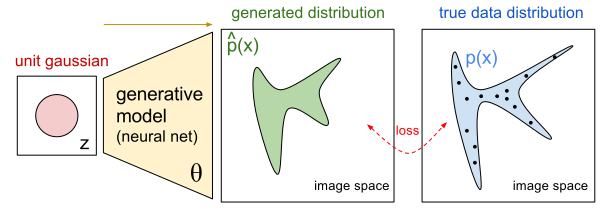
\includegraphics[width=1\columnwidth]{figures/generative_model_math.png}
	\caption{Általános generatív modell tanítása. (forrás: \cite{fig:generative_model_math})}
	\label{fig:data_distribution}
\end{figure}

%-------
% Now, it is not always possible for our machine to learn the true distribution of the data, for this, we take the help of a powerful neural network which can help make the machine learn the approximate true distribution of the data. The neural networks we use as generative models have parameters which are smaller than the amount of data we have as training dataset. The models are forced to discover the distribution in order to generate data.
%-------

A generatív modellek általában kétféle sűrűségbecslést használnak. Explicit Sűrűségbecslés (EDE), és Implicit Sűrűségbecslés (IDE) \cite{goodfellow2016nips}. Az EDE-ben előre meghatározott sűrűségfüggvényeket használnak a megfigyelések és valószínűségeik közötti kapcsolat közelítésére. Ezek a függvények paramétereik változtatásával illeszthetőek a megfigyelésekre. Például normális eloszlás két paramétere: várható érték és szórás állításával illeszthető az adatra. Aze IDE-ben nem előre meghatározott sűrűségfüggvényeket használnak, hanem egy algoritmust használnak a valószínűségi eloszlás közelítésére. Ennek egy példája kernel sűrűségbecslés. Bár az IDE módszerek is paramétereket használnak a közelítéshez, ezeket nem lehet közvetlenül manipulálni mint az EDE esetén. A \ref{fig:gen_models_tax}. ábra a különböző generatív modellek rendszerezését mutatja be az alkalmazott sűrűségbecslés típusa szerint.

% Generative Adversial Network (GAN) is an Implicit density based generative model. Variational Autoencoder (VAE) and Boltzmann Machine (BM) are the explicit density based generative models.  

% Two types of density estimations are generally used in generative models; Explicit Density Estimation (EDE) and Implicit Density Estimation (IDE). In EDE, predefined density functions are used to approximate the relationship between observations and their probability. The observed data is fit to predefined function by manipulating a fixed set of parameters of the function. An example is trying to fit given data to normal distribution using mean and the standard deviations of the samples. This type of density estimation is also known as parametric density estimation. In IDE, predefined density functions are not used. Instead an algorithm is used to approximate the probability distribution of the data. Kernel density approximation is an example of this type. Though the IDE methods use parameters for approximation, they cannot be directly manipulated the way they are in EDE. Figure 3 shows the taxonomy of different generative models based on the type of density estimation used.

\begin{figure}[ht]
	\centering
	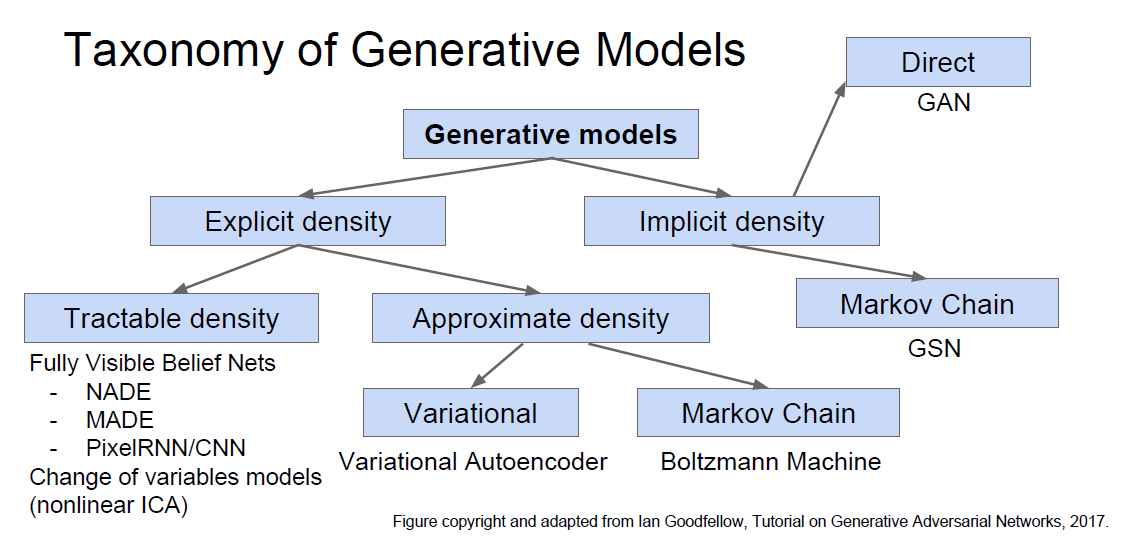
\includegraphics[width=1\columnwidth]{figures/generative_model_taxonomy.png}
	\caption{Generatív modellek fajtái \cite{goodfellow2016nips}.}
	\label{fig:gen_models_tax}
\end{figure}


%----------------------------------------------------------------------------
%----------------------------------------------------------------------------
\subsection{Boltzman gépek}

A következő részben a generatív modellek egyik fajtáját: a Boltzman gépet (BM) működését, illetve annak egyik változatát, a Restricted Boltzman gépet (RBM) mutatom be, de előtte néhány alapvető fogalmat mutatok be amik szükségesek a BM megértéséhez.

% A jelenlegi cikkben a generatív modellekre fogunk összpontosítani, különösen a Boltzmann Machine (BM), népszerű változata a Restricted Boltzmann Machine (RBM), az RBM működésére és néhány alkalmazására. Mielőtt elmélyülne a BM részleteiben, megvitatunk néhány alapvető fogalmat, amelyek elengedhetetlenek a BM megértéséhez.

% In the current article we will focus on generative models, specifically Boltzmann Machine (BM), its popular variant Restricted Boltzmann Machine (RBM), working of RBM and some of its applications. Before deep-diving into details of BM, we will discuss some of the fundamental concepts that are vital to understanding BM. 

% BMs are useful to extract latent space from the data. The difference is in the architecture, the representation of the latent space and the training process. 

%----------------------------------------------------------------------------
\subsubsection{Markov-lánc}

A matematikában a Markov-lánc egy olyan diszkrét sztochasztikus folyamatot jelent, amely Markov-tulajdonságú. Nevét egy orosz matematikusról, Andrej Markovról kapta, aki hírnevét a tudomány ezen ágában végzett kutatásaival szerezte. Markov-tulajdonságúnak lenni röviden annyit jelent, hogy adott jelenbeli állapot mellett, a rendszer jövőbeni állapota nem függ a múltbeliektől. Másképpen megfogalmazva ez azt is jelenti, hogy a jelen leírása teljesen magába foglalja az összes olyan információt, ami befolyásolhatja a folyamat jövőbeli helyzetét. Példa képpen: a véletlenszerűen sétáló személy helyzete a $t+1$ pillanatban a $t$ aktuális állapottól függ, és nem a korábbi állapotoktól $(t-1, t-2,\dots)$. Ezt a viselkedést Markov tulajdonságnak nevezik.

% A Markov chain is a probabilistic model used to estimate a sequence of possible events in which the probability of each event depends only on the state attained in the previous event.  In a Markov chain, the future state depends only on the present state and not on the past states. An example of Markov’s process is show in figure 4.  The position of the randomly walking person at instant t+1 is dependent on the current state t and not on the previous states (t-1, t-2, …..). This behavior is referred to as Markov property.

% \begin{figure}[ht]
% 	\centering
% 	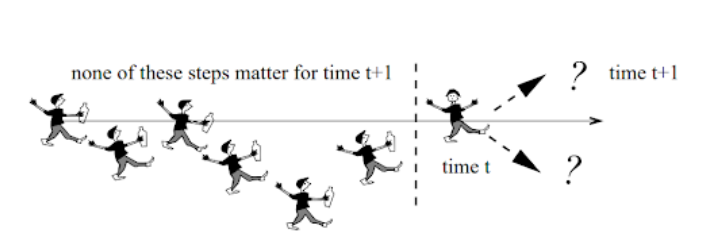
\includegraphics[width=1\columnwidth]{figures/markov_chain.png}
% 	\caption{abra alatti szoveg}
% 	\label{fig:markov}
% \end{figure}


%----------------------------------------------------------------------------
\subsubsection{Grafikus modell}

A grafikus valószínűségi modell egy grafikus ábrázolás, amivel véletlen változók közötti feltételes valószínűséget lehet kifejezni. A grafikus modellnek két fő komponense van: csúcsok és élek. A csúcsok a véletlen változó állapotát jelzik, míg az élek az átalakulás irányát. Az ilyen gráfoknak két fő típusa van: irányított és irányítatlan. A \ref{fig:graph}. ábrán látható példán egy csecsemő táplálkozási szokásainak Markov folyamatának irányítatlan grafikus modelljét láthatjuk. A baba következő étkezésének kiválasztása kizárólag attól függ, hogy mit eszik most, és nem attól, amit korábban evett.

\begin{figure}[ht]
	\centering
	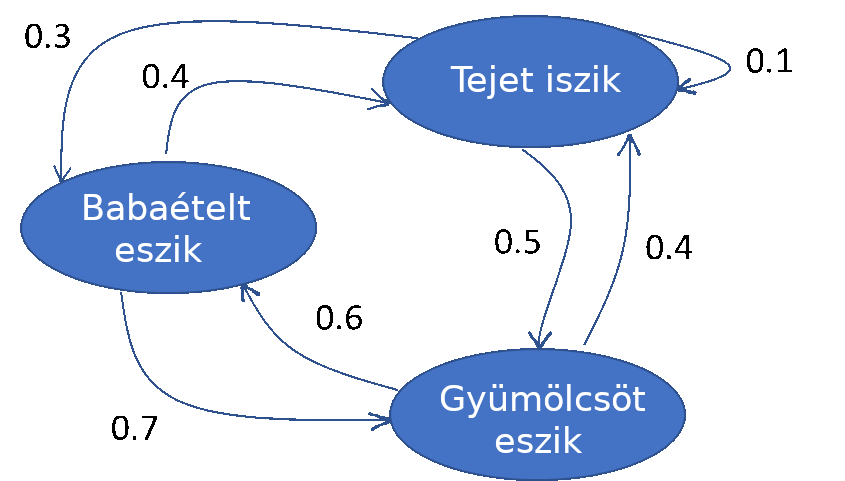
\includegraphics[width=0.7\columnwidth]{figures/graph_example.png}
	\caption{Példa grafikus ábrára.}
	\label{fig:graph}
\end{figure}

%https://en.wikipedia.org/wiki/Graphical_model

% A grafikonmodell segítségével jelezhetjük a baba választását a következő étkezéshez a valószínűségekkel együtt. A baba következő étkezésének kiválasztása kizárólag attól függ, hogy mit eszik most, és nem attól, amit korábban evett. Annak valószínűségét, hogy egy adott ételt választanak a következő étkezéshez, történelmi megfigyelések alapján számítják ki.

% A graphical probabilistic model is a graphical representation used to expresses the conditional dependency between random variables. A graphical model has two components in it; Vertices and edges. The vertices indicate the state of random variable and the edge indicates direction of transformation. The two main types of computational graphs; directed and undirected. Figure 6 shows an undirected graphical model of a Markov process of diet habit of a baby. The graph model is used to indicate a baby’s choice for the next meal with the associated probabilities. The baby’s choice of next meal depends solely on what it is eating now and not what it ate earlier. The probability of choosing a specific food for next meal is calculated based on historic observations.

%-------

Egy Markov tulajdonsággal rendelkező irányítatlan gráf által leírt valószínűségi változók halmazát Markov hálózatnak (Markov Random Field az angol szakirodalomban). A Boltzman gépek is a MRF-ek közé tartozik.

A Boltzman gép egy probabilisztikus generatív irányítatlan gráfmodell, amely kielégíti a Markov tulajdonságot. A BM-ek megtanulják a tanító minták eloszlását, majd abból új mintákat tudnak generálni. A BM rendelkezik bemeneti réteggel (látható réteggel) és egy vagy több rejtett réteggel. Kimeneti rétege nincs. A \ref{fig:bm}. ábrán láthatunk egy tipikus egy rejtett réteget tartalmazó Boltzman gépet.

% A Markov tulajdonsággal rendelkező és egy nem irányított gráf által leírt véletlen változók halmazát Markov Random Field (MRF) vagy Markov hálózatnak nevezzük. Más szavakkal, egy véletlen mező Markov véletlenszerű mező, ha kielégíti Markov tulajdonságát. A BM egyfajta MRF.

% A Boltzmann -gép (BM) egy valószínűségi generatív irányítatlan gráfmodell, amely kielégíti Markov tulajdonságát. A BM -ek megtanulják a valószínűségi sűrűséget a bemeneti adatoktól az új minták generálásáig azonos eloszlásból. A BM rendelkezik bemeneti vagy látható réteggel és egy vagy több rejtett réteggel. Nincs kimeneti réteg. A 6. ábra egy rejtett rétegű BM tipikus architektúráját mutatja.

% A set of random variables having Markov property and described by an undirected graph is referred to as Markov Random Field (MRF) or Markov network. In other words, a random field is said to be a Markov random field if it satisfies Markov property. BM is a type of MRF.

% We now have a grasp on some of the fundamental concepts to understand BM. A Boltzmann Machine (BM) is a probabilistic generative undirected graph model that satisfies Markov property. BMs learn the probability density from the input data to generating new samples from the same distribution. A BM has an input or visible layer and one or several hidden layers. There is no output layer. Figure 6 shows a typical architecture of a BM with single hidden layer. 

A hálózat neuronjai megtanulnak sztochasztikus döntéseket hozni akkór, hogy be vagy kikapcsoljanak a tanítás során látott mintáknak megfelelően. Így a BM-ek fel tudják fedni a tanító adatok összetett mögöttes mintázatait. Lényeges különbség a BM és az egyéb neurális hálózat architektúrák között az, hogy a BM neuronjai nemcsak más rétegek neuronjaihoz kapcsolódnak, hanem ugyanazon a rétegen belüli neuronokhoz is, minden neuron kapcsolódik a hálózat összes többi neuronhoz. Ezt azt architektúrát Korlátlan Boltzman Gépnek nevezik, aminek a tanítása rendkívűl nehézkes és e miatt kevés gyakorlati haszna van. Az azonos rétegbeli idegsejtek közötti kapcsolatok megszüntetésével egy más architektúrát kapunk amit Korlátozott Boltzman Gépnek (RMB) hív a szakirodalom. A gyakorlatban az RBM-et használják, mert a hálót könyebb tanítani. A BM és RBM közötti különbséget a \ref{fig:bm}. ábra szemlélteti.

\begin{figure}[ht]
	\centering
	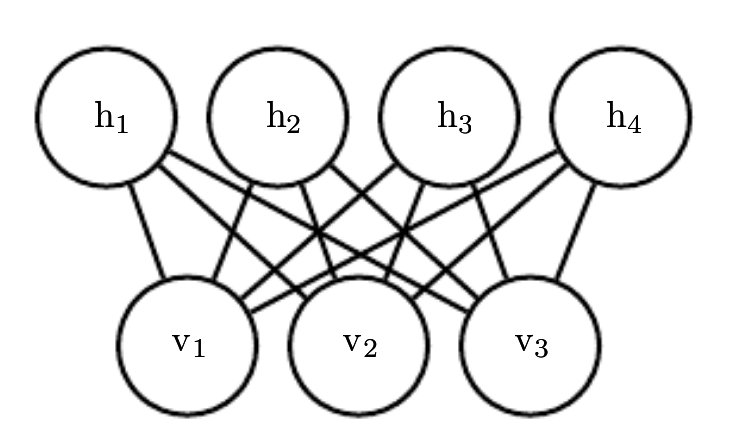
\includegraphics[width=0.50\columnwidth]{figures/RBM.png}
	\caption{A korlátozott Boltzman gép (RBM) egy kétirányú gráfon alapuló irányítatlan grafikus modell, aminek egyik részén a látható elemek vannak (v), a másik részén a rejtett elemek (h). (forrás: \cite{fig:RMB})}
	\label{fig:bm}
\end{figure}

% The neurons in the network learn to make stochastic decisions about whether to turn on or off based on the data fed to the network during training.  This helps the BM discover and model the complex underlying patterns in the data. A vital difference between BM and other popular neural net architectures is that the neurons in BM are connected not only to neurons in other layers but also to neurons within the same layer. Essentially, every neuron is connected to every other neuron in the network.  This imposes a stiff challenge in training a BM and this version of BM, referred to as ‘Unrestricted Boltzmann Machine’ has very little practical use. Eliminating the connections between the neurons in the same layer relaxes the challenges in training the network and such networks are called as Restricted Boltzmann Machine (RBM). In practice, RBMs are used in verity of applications due to simpler training process compared to BMs

% \subsubsection{Energy based model}
%~~~~~~~~
% Boltzmann Machines are primarily divided into two categories: Energy-based Models (EBMs) and Restricted Boltzmann Machines (RBM). When these RBMs are stacked on top of each other, they are known as Deep Belief Networks (DBN).
%~~~~~~~~~ (https://medium.com/machine-learning-researcher/boltzmann-machine-c2ce76d94da5)

%~~~~~~
% Energy is a term that may not be associated with deep learning in the first place. Rather is energy a quantitative property of physics. E.g. gravitational energy describes the potential energy a body with mass has in relation to another massive objected due to gravity. Yet some deep learning architectures use the idea of energy as a metric for the measurement of the model’s quality.
% One purpose of deep learning models is to encode dependencies between variables. The capturing of dependencies happens through associating of scalar energy to each configuration of the variables, which serves as a measure of compatibility. High energy means bad compatibility. An energy-based model tries always to minimize a predefined energy function. The energy function for the RBMs is defined as:

%equation :)
 
% As can be noticed the value of the energy function depends on the configurations of visible/input states, hidden states, weights, and biases. The training of RBM consists of the finding of parameters for given input values so that the energy reaches a minimum.
%~~~~~~ (https://medium.com/machine-learning-researcher/boltzmann-machine-c2ce76d94da5)

% \subsubsection{Training}
% ha kell még content
%----------------------------------------------------------------------------
\subsubsection{RBM alkalmazásai}

Az mély tanulás első napjaiban az RBM-eknek különféle feladatoknál alkalmazták, mint például dimenziócsökkentéshez, vagy ajánlórendszerekhez vagy természetes nyelv feldolgozásra. Néhány alkalmazási példa RBM-re:
\begin{itemize}
	\item Mintázat felismerés: Az RBM jellemzők kinyerésére (feature extraction) alkalmas mintázatfelismerési problémák esetén, amikor kézzel írott szöveg felismerése a cél. [REF]
	\item Anánlórendszerek: Az RBM-eket széles közben használják olyan feladatokra, ahol megjósolják, hogy mit érdemes ajánlani a felhasználónak ami számára hasznos lenne, és ezért szívesen használja az alkalmazást. Példa: filmajánlás, zeneajánló. [REF]
\end{itemize}

Azonban az utóbbi időkben a gyakorlatban az RBM-eket szinte teljesen felváltották a Generatív Adversarial Network-ök (GAN), vagy a Variational Autoencoderek (VAE).

% Pattern recognition : RBM is used for feature extraction in pattern recognition problems where the challenge is to understand the hand written text or a random pattern. 
% Recommendation Engines : RBM is widely used for collaborating filtering techniques where it is used to predict what should be recommended to the end user so that the user enjoys using a particular application or platform. For example : Movie Recommendation, Book Recommendation
% Radar Target Recognition : Here, RBM is used to detect intra pulse in Radar systems which have very low SNR and high noise.

% During the early days of deep learning, RBMs were used to build a variety of applications such as Dimensionality reduction, Recommender systems, Topic modelling. However, in recent times, RBMs have been almost replaced by Generative Adversarial Networks (GANs) or Variation Autoencoder (VAEs) in different machine learning applications.

%----------------------------------------------------------------------------
\subsection{Generatív Adversarial Network}
%----------------------------------------------------------------------------

A Generatív Adversarial Network (más néven GAN) az utóbbi évek egyik innovációja a mély tanulás területén. A GAN-okat eredetiel Ian Goodfellow és Yoshua Gengio vezették be a Montreali Egyetemen, 2014-ben. A GAN-ok célja egy eloszlás megtanulása, és abból új példányok generálása.

A GAN egy generatív modell, amelyben két neurális háló verseng egymással. Az első hálót generátornak nevezik. A generátor felelős új szintetikus minták előállításáért, amelyek hasonlítanak a tanító halmaz mintáihoz. A másik neurális hálót diszkriminátornak nevezik, aminek a feladata megkülönböztetni a valódi minták (tanító minta) illetve a generátor által létrehozott szintetikus minták között. A generátor célja becsapnia a diszkriminátort, míg a diszkriminátor megpróbál ennek ellenállni. A két háló versengéséből ered az ``adversarial'' elnevezés.

Az alábbi \ref{fig:gan_struct}. ábrán látható, hogy a generátor nem találkozik a tanító mintákkal, csupán véletlen zajt kap a bemenetére. A diszkriminátor hozzáfér a tanító adatokhoz osztályozás céljából. A generátor képes javítani a kimenetén kizárólag a diszkriminátortól kapott visszajelzés alapján (pozitív, ha a tanító mintával egyezik a kimenet, negatív ha nincs egyezés).

%~~~~~~~~~~~~~~~~~~
% Generative Adversarial Networks (a.k.a. GANs) represents one of the most exciting recent innovation in deep learning. GANs were originally introduced by Ian Goodfellow and Yoshua Bengio from the University of Montreal, in 2014.

% A GAN is a generative model in which two neural networks are competing in a typical game theory scenario. The first neural network is the generator, responsible of generating new synthetic data instances that resemble your training data, while its adversary, the discriminator tries to distinguish between real (training) and fake (artificially generated) samples generated by the generator. The mission of the generator is to try fooling the discriminator, and the discriminator tries to resist from being fooled. That’s why the system as a whole is described as adversarial.

% As shown in the figure below, the generator’s input is simply a random noise, while, only the discriminator has access to the training data for classification purposes. The generator keeps improving its output based, exclusively, on the feedback of the discriminator network (positive in case of match with training data and negative if there is no match). The goal for these generated data samples is to be the fair samples from the distribution of real data.
%~~~~~~~~~~~~~~~~~~
% Generative adversarial networks, also known as GANs are deep generative models and like most generative models they use a differential function represented by a neural network known as a Generator network. GANs also consist of another neural network called Discriminator network.

% A Generator network takes random noise as input and runs that noise through the differential function to transform the noise and reshape it to get a recognisable structure. The output of the generator seems like a real data point. The choice of the random input voice determines which data point will come out of the generator network. Running the generator network with many different input noise values produces many different realistic output data samples. The goal for these generated data samples is to be the fair samples from the distribution of real data.

\begin{figure}[ht]
	\centering
	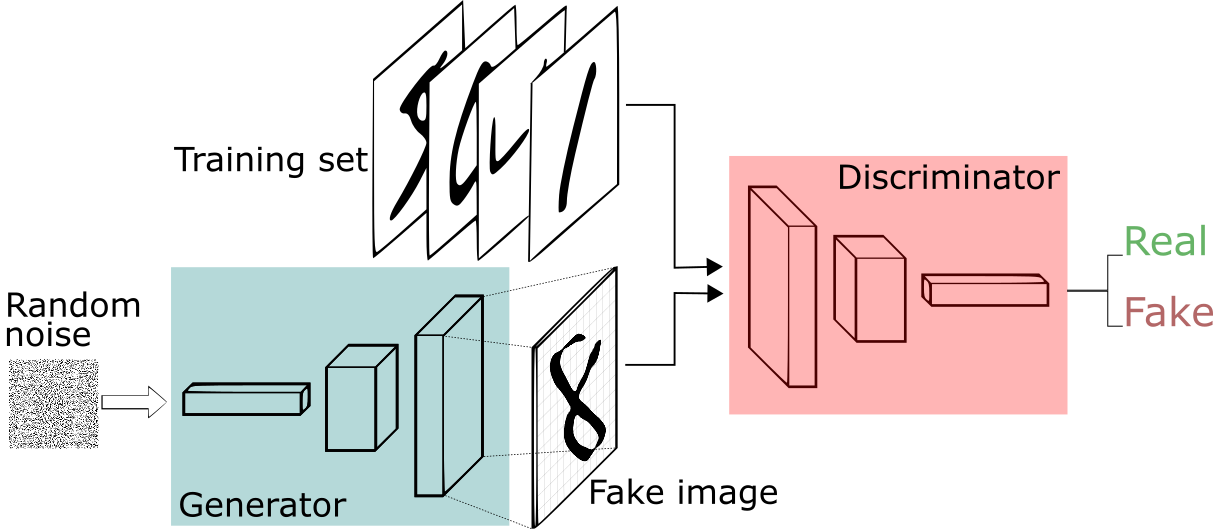
\includegraphics[width=0.9\columnwidth]{figures/gan_struct.png}
	\caption{A GAN általános struktúrája. (forrás: \cite{fig:gan_struct})}
	\label{fig:gan_struct}
\end{figure}

\subsubsection{GAN tanítása}

A generátor be kell tanítani, mielőtt realisztikus mintákat képes létrehozni. Tegyük fel, hogy egy újonnan inicializált hálót használunk 200 kép előállítására, minden mintánál új random zaj bemenettel. Mivel a generatív modell tanítása felügyelet nélküli, nincsenek címkéink amivel össze lehetne vetni a háló kimenetét. Honnan tudjuk mégis, hogy milyen irányba kell módosítani a háló paramétereit, hogy javuljon a generált képek minősége? Egy generált kép ``jóságát'' nem külsőleg mondjuk meg (címke segítségével), hanem az dönti el, hogy sikerült-e átverni a diszkriminátort.

A diszkriminátor háló ad visszajelzést a generátornak tanulás során, hogy meg tudja tanulni az adott minták eloszlását. A diszkriminátor tipikusan egy osztályozó konvolúciós neurális háló ami képes megkülönböztetni a generált mintákat a valós mintáktól. A tanítás során a diszkriminátornak az esetek felében valódi mintákat, a másik felében szintetikus mintákat lát. A valós mintákhoz 1-hez közeli valószínűséget, hamis mintákhoz pedig 0-hoz közelit rendel. A generátor e közben megtanul olyan mintákat generálni, amelyekre a diszkriminátor 1-hez közeli kimenetet produkál, és valódi mintának minősítené azt. Idővel a generátor kénytelen egyre realisztikusabb kimeneteket előállítani, hogy meg tudja téveszteni a diszkriminátort. Ezzel a módszerrel egy felügyelet nélküli tanulási feladatot sikerül visszavezetni egy felügyelt tanulási feladatra.

% GAN -k közelítést használnak, ahol a második hálózat, a Diszkriminátor, a Generator -t vezeti, hogy a mintákat előállítsa az adott adatok valószínűségi eloszlásából. A diszkriminátor egy rendszeres neurális hálózat osztályozó, amely a valódi mintákat a generátor által generált hamis mintákból osztályozza. A képzési folyamat során a diszkriminátornak az idő felében valódi mintákat, a másik felében pedig hamis mintákat jelenítenek meg a generátorból. Valós mintákhoz 1 -hez közeli valószínűséget, hamis mintákhoz pedig 0 -hoz közeli valószínűséget rendel. Eközben a generátor olyan mintákat próbál kiadni, amelyeket a diszkriminátor közel egy valószínűséggel rendelne hozzá, és valódi mintáknak minősítené őket. Idővel a generátor kénytelen a reálisabb kimenetű mintákat előállítani a megkülönböztető félrevezetése érdekében. Ne feledje, hogy ez az ellentmondásos keret átalakította a nyers adatok és a minták nélküli felügyelet nélküli problémát az általunk létrehozott címkék által felügyelt problémává, azaz valódivá és hamisá.

% ~~~~~~~~~~~~
% The generator network needs to be trained before it can generate realistic data points as output. The training process for a generative model is different from that of the training process of a supervised model. For a supervised learning model, each input data is associated with its respective label whereas, for a generative model, the model is shown a lot of data samples and it makes new data samples that come from the same probability distribution.

% GANs use an approximation where a second network called the Discriminator guides the Generator to  generate the samples from the probability distribution of given data. The Discriminator is a regular neural network classifier that classifies the real samples from the fake samples generated by the Generator. During the training process, the Discriminator is shown real samples half of the time and fake samples from the Generator the other half of the time. It assigns a probability close to ‘1’ to real samples and the probability close to ‘0’ to fake samples. Meanwhile, the Generator is trying to output samples that the Discriminator would assign a probability of near one and classify them as real samples. Over time the generator is forced to produce the samples that are more realistic outputs in order to fool the Discriminator. Note that this adversarial framework has transformed an unsupervised problem with raw data and no samples into a supervised problem with labels we create, that is, real and fake. 

% ~~~~~~~~~~~~~ about training
% Suppose that we used a newly-initialized network to generate 200 images, each time starting with a different random code. The question is: how should we adjust the network’s parameters to encourage it to produce slightly more believable samples in the future? Notice that we’re not in a simple supervised setting and don’t have any explicit desired targets for our 200 generated images; we merely want them to look real. One clever approach around this problem is to follow the Generative Adversarial Network (GAN) approach. 
% Here we introduce a second discriminator network (usually a standard convolutional neural network) that tries to classify if an input image is real or generated. For instance, we could feed the 200 generated images and 200 real images into the discriminator and train it as a standard classifier to distinguish between the two sources. But in addition to that — and here’s the trick — we can also backpropagate through both the discriminator and the generator to find how we should change the generator’s parameters to make its 200 samples slightly more confusing for the discriminator. These two networks are therefore locked in a battle: the discriminator is trying to distinguish real images from fake images and the generator is trying to create images that make the discriminator think they are real. In the end, the generator network is outputting images that are indistinguishable from real images for the discriminator.
%~~~~~~~~~~~~~~ (https://openai.com/blog/generative-models/)

%~~~~~~~~~~~~~
% Generative adversarial networks (GANs), are a relatively new deep learning architecture for neural networks. They were pioneered by Ian Goodfellow and his colleagues at the University of Montreal in 2014. A GAN trains two different networks, one against the other, hence they are adversarial. One network generates an image (or any other sample, such as text or speech) by taking a real image and modifying it as much as it can. The other network tries to predict whether the image is “fake” or “real.” The first network, called the G network, learns to generate better images. The second network, the D network, learns to discriminate between the fake and real images. Its ability to discriminate improves over time. 
%~~~~~~~~~~~~~ (https://aws.amazon.com/blogs/machine-learning/combining-deep-learning-networks-gan-and-siamese-to-generate-high-quality-life-like-images/)


% ez az abra nem jön be az oldalról
\begin{figure}[ht]
	\centering
	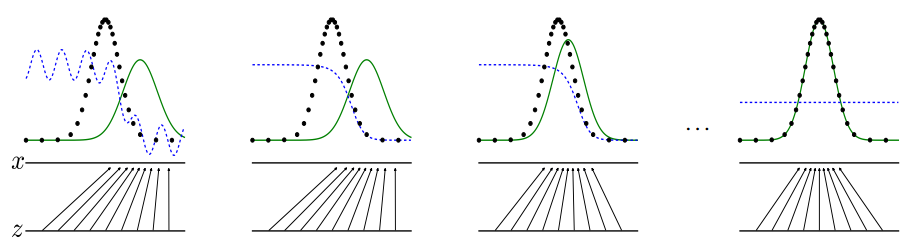
\includegraphics[width=1\columnwidth]{figures/gan_dist.png}
	\caption{Tanulás folyamata. Kék pontozott vonal jelöli a diszkriminátor eloszlását, zöld folytonos vonal a generált minták eloszlását, a fekete görbe pedig a tanító adat eloszlását \cite{fig:gan_dist}.}
	\label{fig:gan_dist}
\end{figure}

A \ref{fig:gan_dist}. ábrán láthatjuk a GAN tanulásának folyamatát. A generátor $z$ véletlen zaj értéket kap bemenetre, és azt leképezi az $x$ kimeneti értékre. Az $x$ értékeinek eloszlása sűrűbbé válik, ahova több $z$ értéket képezünk le. A diszkriminátor magas értéket ad azokon a helyeken, ahol a valódi adatok sűrűsége nagyobb, mint a generált adatoké. A generátor a háló paramétereinek változtatásával módosítani tud a leképezésen, és így eléri, hogy az eloszlása a diszkriminátor gradiens irányába változzon. Végül a generátor eloszlása megegyezik a valós minták eloszlásával. Ekkor a diszkriminátor minden mintára 0,5-ös valószinűséget ad, mivel nem tudja megkülönböztetni a valós és generált mintákat.

% The Generator takes random noise value z and maps them to output values x. The probability distribution over x represented by the model becomes denser wherever more values of z are mapped. The Discriminator outputs high values wherever the density of real data is greater than the density of generated data. The Generator changes the samples it produces to move uphill along the function learned by the Discriminator and eventually the Generator’s distribution matches the distribution of real data. Due to this, the Discriminator outputs the probability of 0.5 for every sample because every sample is equally likely to be generated by the real data-set as it is to be generated by the Generator.

% We can think of this process as a competition between police and counterfeiters. The Generator network is like a counterfeiter trying to produce fake money and pass it off as real. The police act as a Discriminator network and want to catch the counterfeiter spending the fake money but also do not want to stop people using real money. Over time the police get better at recognising fake money but at the same time, the counterfeiter also improves his techniques to produce fake currency. At some point, the counterfeiter makes exact replicas of the currency and the police can no longer discriminate between the real and fake money.

A GAN-oknak annak ellenére, hogy nemrég jelentek csak meg, gyakorlati hasznuk is van. Erre pár példa:
\begin{itemize}
	\item \textbf{StyleGan3}: Ez egy GAN-on alapuló neurális háló, amely képes az fotorealisztikus emberi arcképeket generálni. \cite{stylegan3}
	\item Egy 2018-as aukción egy GAN által ``festett'' kép több mint \$400 ezer dollárért kelt el \cite{AIart}. 
\end{itemize}

%----------------------------------------------------------------------------
\subsection{Generatív Autoenkóderek}

Az autoenkóderek olyan neurális hálók, ahol a kimeneti réteg mérete megegyezik a bemeneti réteg méretével. Az autoenkóder felügyelet nélküli tanulásra képes, feladata minél kisebb veszteséggel visszaállítsa a bemenetre érkező adatot, ezért replikátor neurális hálónak is nevezik.

% Autoencoder is a type of neural network where the output layer has the same dimensionality as the input layer. In simpler words, the number of output units in the output layer is equal to the number of input units in the input layer. An autoencoder replicates the data from the input to the output in an unsupervised manner and is therefore sometimes referred to as a replicator neural network.

% Az automatikus kódolók a bemenet minden dimenzióját úgy rekonstruálják, hogy átviszik a hálózaton. Lehet, hogy triviálisnak tűnik a neurális hálózat használata a bemenet replikálására, de a replikációs folyamat során a bemenet mérete kisebbre csökken. A neurális hálózat középső rétegei kevesebb egységgel rendelkeznek, mint a bemeneti vagy kimeneti rétegek. Ezért a középső rétegek tartják a bemenet csökkentett ábrázolását. Belsőleg rejtett réteggel rendelkezik, amely leírja a bemenet ábrázolásához használt kódot. A kimenet a bemenet ezen csökkentett ábrázolásából rekonstruálódik.

% The autoencoders reconstruct each dimension of the input by passing it through the network. It may seem trivial to use a neural network for the purpose of replicating the input, but during the replication process, the size of the input is reduced into its smaller representation. The middle layers of the neural network have a fewer number of units as compared to that of input or output layers. Therefore, the middle layers hold the reduced representation of the input. Internally, it has a hidden layer that describes a code used to represent the input. The output is reconstructed from this reduced representation of the input.

A háló tartalmaz egy $\textbf{h}$ rejtett réteget, ami a bemenet belső leképezését tárolja. A háló két részből tevődik össze: egy kódoló függvényből $\textbf{h} = f(\textbf{x})$, és egy dekódolóból, amely rekonstruálja a bemenetet $\textbf{r} = g(\textbf{h})$. Ha az autoenkóder egyszerűen megtanulná a $g(f(\textbf{x})) = \textbf{x}$ függvényt, az nem lenne túl hasznos, ezért a kódolót úgy tervezték, hogy képtelenek legyenek a bemenetet tökéletesen másolni. A kódolót úgy korlátozzák, hogy a középső rejtett réteg kevesebb neuront tartalmaz mint a bemeneti réteg. Ennek hatására a kódoló kénytelen priorizálni, hogy a bemenet mely jellemzőit érdemes másolni, így képes megtanulni az adatok hasznos tulajdonságait.

Az autoenkóderek tipikus felépítése: (látsd: \ref{fig:autoenc_struct}. ábra).

% A hálózat két részből tevődik össze: egy anenkódoló függvény = f (x) és egy dekódoló, amely rekonstrukciót eredményez = g (h). Ezt az architektúrát a 14.1. Ábra mutatja be. Ha egy automatikus kódolónak sikerül egyszerűen megtanulnia a setg (f (x)) = x mindenhol, akkor ez nem különösen hasznos. Ehelyett az automatikus kódolókat úgy tervezték, hogy képtelenek legyenek megtanulni tökéletesen másolni. Általában olyan módon korlátozzák őket, amelyek lehetővé teszik számukra, hogy csak hozzávetőlegesen másoljanak, és csak olyan adatokat másoljanak be, amelyek hasonlítanak az edzési adatokhoz. Mivel a modell kénytelen priorizálni, hogy a bemenet mely aspektusait kell másolni, gyakran megtanulja az adatok hasznos tulajdonságait

%~~~~~~~~~~~~~~~~~~~~~~~
% Internally, it has a hidden layerhthat describes acodeused torepresent the input. The network may be viewed as consisting of two parts: anencoder function=f(x) and a decoder that produces a reconstructionr=g(h).This architecture is presented in figure 14.1. If an autoencoder succeeds in simplylearning to setg(f(x)) =xeverywhere, then it is not especially useful. Instead,autoencoders are designed to be unable to learn to copy perfectly. Usually they are restricted in ways that allow them to copy only approximately, and to copy onlyinput that resembles the training data. Because the model is forced to prioritize which aspects of the input should be copied, it often learns useful properties of thedata
  
%~~~~~~~~~~~~~~~~~~~~~~ (https://www.deeplearningbook.org/contents/autoencoders.html)

% An autoencoder consists of three components:

\begin{figure}[ht]
	\centering
	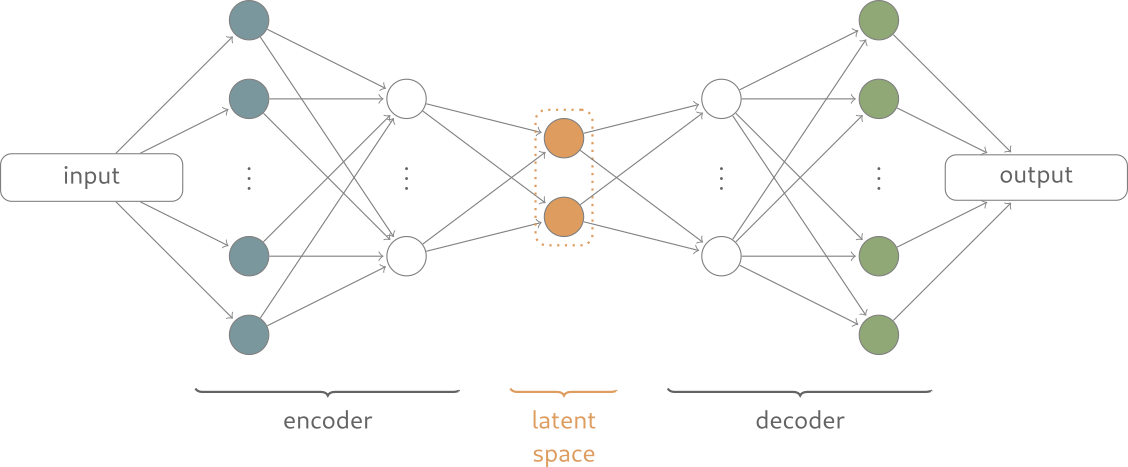
\includegraphics[width=1\columnwidth]{figures/ae.png}
	\caption{Az autoenkóder részei: enkóder, kód (látens tér) és dekódoló (forrás: \cite{fig:autoenc_struct})}
	\label{fig:autoenc_struct}
\end{figure}

\begin{itemize}
	\item \textbf{Kódoló}: A kódoló egy előrecsatolt, teljesen kapcsolt neurális háló, amely a bemenetet látens térbeli reprezentációba tömöríti. A bemeneti képet tömörített ábrázolásként kódolja csökkentett méretben.
	\item \textbf{Kód}: A hálózat ezen része tartalmazza a dekódolóba táplált bemenet csökkentett ábrázolását. (más néven látens változók).
	\item \textbf{Dekódoló}: A dekódoló a kódolóhoz hasonló struktúrájú előrecsatolt háló. Feladata kód alapján a bemenet visszaállítása.
\end{itemize}

Az autoenkóderek évtizedek óta ismertek a neurális hálózatok világában [REF]. Míg eleinte az autoenkódereket dimenziócsökkentéshez, vagy jellemző tanuláshoz használták, a közelmúltban a generatív modellezésben is előtérbe került. Az első komoly generatív tulajdonsággal rendelkező autoenkódert a variációs autoenkóder megjelenése hozta.

% A modern autókódolók a determinisztikus funkciókon túli kódoló és dekódoló ötletét a sztochasztikus leképezésekre (h | x) és pdekódolókra (x | h) általánosították. Az automatikus kódolók ötlete évtizedek óta része a neurális hálózatok történelmi tájának (LeCun , 1987; Bourlard és Kamp, 1988; Hinton és Zemel, 1994). Hagyományosan az automatikus kódolókat használták a dimenziócsökkentéshez vagy a funkciók tanulásához. A közelmúltban az autokódolók és a változó modellek közötti elméleti kapcsolatok az autokódolókat a generációs modellezés előtérébe hozták.

% Modern autoencoders have generalized the idea of an encoder and a de-coder beyond deterministic functions to stochastic mappingspencoder(h | x) andpdecoder(x | h).
% The idea of autoencoders has been part of the historical landscape of neuralnetworks for decades (LeCun, 1987; Bourlard and Kamp, 1988; Hinton and Zemel,1994). Traditionally, autoencoders were used for dimensionality reduction orfeature learning. Recently, theoretical connections between autoencoders andlatent variable models have brought autoencoders to the forefront of generativemodeling

\subsubsection{Variációs autoenkóderek}

A variációs autoenkóder (VAE) megjelenése nem túl régi, 2013-ban publikálták először \cite{kingma2013auto}. Bár mély neurális háló alapú autoenkóderek korábban is léteztek, mint generatív modell rosszul teljesítettek. Később azonban képgenerálás [REF], és megerősítéses tanulás [REF] területén is előremutató eredmények születtek.

% Az első komoly generatív tulajdonsággal rendelkező autóenkóder, a Variációs Au- tóenkóder (továbbiakban VAE) megjelenése nem túl régi: [25] [26] pulikálták elő- ször 2014-ben. Bár mély mesterséges háló alapú autóenkóderek előtte is léteztek, mint generatív modell azonban rosszul teljesítettek. Később azonban a képgenerálás, és a megerősítéses tanulás [27] területén is előremutató eredmények születtek.

%We add a constraint on the encoding network, that forces it to generate latent vectors that roughly follow a unit gaussian distribution. It is this constraint that separates a variational autoencoder from a standard one.

%TODO ezt újraírni h érthető legyen
A variációs autoenkóder annyiban tér el a standard autoenkódertől, hogy adunk egy megkötést a kódolónak, aminek hatására a generált látens változók vektora ($\textbf{h}$) közel követik a normális eloszlást. Ebben az esetben a normális eloszlás $\mathcal{N}(\mu,\sigma^2)$ várható értéke ($\mu$) és szórásnégyzete ($\sigma^2$) leírja a látens változók eloszlását. Ekkor az enkóder és dekóder nem determenisztikus hanem sztohasztikus jellegű. Ez a megkötés azért hasznos számunkra, mert normális eloszlásból könnyen tudunk mintavételezni, ami megkönnyíti az új képek generálását (látsd: \ref{fig:vae}. ábra)

\begin{figure}[ht]
	\centering
	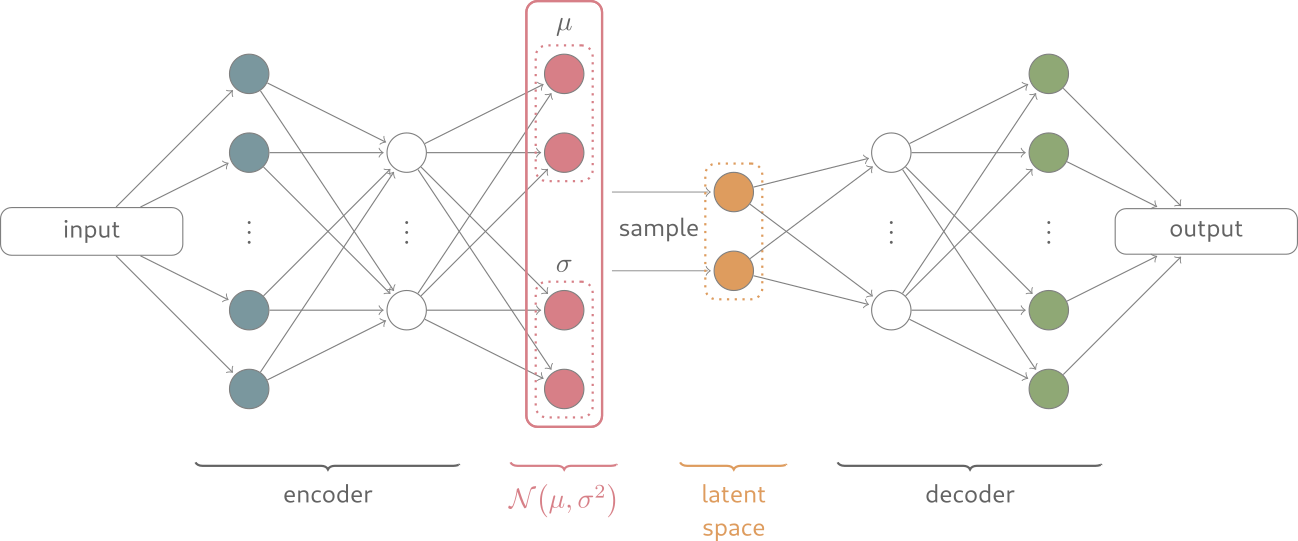
\includegraphics[width=1\columnwidth]{figures/vae.png}
	\caption{A variációs autoenkóder részei. (forrás: \cite{fig:autoenc_struct})}
	\label{fig:vae}
\end{figure}

% Új képek létrehozása most egyszerű: mindössze annyit kell tennünk, hogy mintát veszünk egy látens vektorból a gauss -egységből, és átadjuk a dekódolónak. A gyakorlatban kompromisszum van a hálózatunk pontossága és a látens változóinak közelítő egységei között.

%~~~~~~~~~~~~~~
% There's a simple solution here. We add a constraint on the encoding network, that forces it to generate latent vectors that roughly follow a unit gaussian distribution. It is this constraint that separates a variational autoencoder from a standard one.

% Generating new images is now easy: all we need to do is sample a latent vector from the unit gaussian and pass it into the decoder. In practice, there's a tradeoff between how accurate our network can be and how close its latent variables can match the unit gaussian distribution.
%~~~~~~~~~~~~~~ (https://kvfrans.com/variational-autoencoders-explained/)

A VAE működését könyebb egy példán keresztül bemutatni. Tegyük fel, hogy van egy képünk egy emberi arcról. A betanított háló ez a kép alapján képes látens változó vektort kinyerni a képből, ami az arcot leíró fontos jellemzőkből áll. Erre mutat egy példát a \ref{fig:vae_face}.ábra.

% Let us understand how we are generating new data. Let’s say we have the image of a celebrity face from which our encoder model has to recognize important features mentioned below. 

Mint az alábbi ábrán látjuk, minden jellemzőhöz tartozik egy valószínűségi eloszlás. Miben különböznem az arcok? Megfogalmazhatunk pár ilyen jellemzőt, mint a bőrszín, haj színe, szemek távolsága, stb. Ezen jellemzőkből álló vektor leírhat egy emberi arcot. Eltérő arcoknál a jellemzők értékei mások lesznek, de jellemzők listája ugyanaz marad. Az autoenkóderek nem feltétlenül ilyen ember által könnyen értelmezhető jellemzőket nyer ki az arcokból, hanem azok ennél a példánál absztraktabbak.

\begin{figure}[ht]
	\centering
	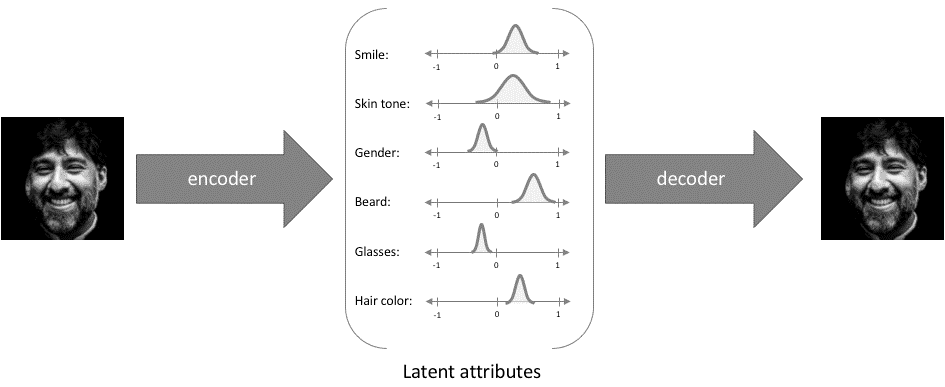
\includegraphics[width=1\columnwidth]{figures/autoenc_latent.png}
	\caption{Látens változók kinyerése a bemeneti arcképből.}
	\label{fig:vae_face}
\end{figure}

Célunk, hogy új képeket állítsunk elő az arcképekből álló tanító mintahalmaz alapján. Feltéve, hogy a bemeneti adataink normális eloszlást követnek, új képek létrehozásához mindössze annyit kell tennünk, hogy normális eloszlásból mintavételezünk egy látens változó vektort. Ezt megadjuk a dekódolónak, ami a vektor alapján generálni tud egy új képet.

%TODO ezt kifejteni ha kell még content, ha nem akkor komment
A VEA számos területen alkalmazott, ezek közül egy példa az úgynevezett ``deepfake'' előállítása, ami lényegében abból áll, hogy egy személy arcát alakítják át úgy, hogy egy másik személy vonásait utánozza. [REF]

% This novel technique allows generating so-called deepfakes, which actually morph a person’s face to mimic someone else’s features, although preserving the original facial expression.

% With every feature, we have a probability distribution. Our goal is to produce new data from the current data or a new face from the current face. How do faces differ? Skin tone, eye colour, hair colour, and many other features are different. But overall, the list of the features remains the same. Since we have a facility with two probability distributions: mean and standard deviations, we have datasets of two new ranges to provide to the decoder.

% As our input data follows a normal distribution, we will be able to provide two variables: mean and variance in the latent space. We want to build a multivariate Gaussian model with the assumption of non-correlation in data which helps us result in a simple vector. Now, provide a set of random samples from mean and variance distributions from latent space to the decoder for the reproduction of data (image).

%if need more / better explonation: https://medium.com/analytics-vidhya/vae-generative-modelling-for-face-recognition-71e8ba16950c

%----------------------------------------------------------------------------
% ARCFELISMERÉS
%----------------------------------------------------------------------------
\subsection{Arcfelismerés neurális hálókkal}

A generatív modellek után áttérnék a modern arcfelismerő rendszerek bemutatására. Mivel a legkorszerűbb arcfelismerő rendszerek mély tanulásra építenek, az ehhez kapcsolódó fogalmakat, neurális háló architektúrákat mutatom be a következő részekben.

\subsubsection{Mély metrika tanulás}
\label{sec:dml}

% TODO mély metrika legyen végig (nem hasonlósági metrika)
% TODO István anyagát belefűzni kicsit

A mély metrika tanulás (angol szakirodalomban: deep metric learning) a felügyelet gépi tanulás azon területe, amelyben a cél egy hasonlósági függvény megtanulása \cite{kaya2019dmlsurvey}. Ez a függvény képes meghatározni két objektumról, hogy mennyire hasonlítanak egymáshoz és hasonlóság mértékét számszerűsíteni tudja. Magasabb hasonlósági értéket ad vissza a függvény, ha az objektumok hasonlóak, és alacsonyabb értéket ad vissza, ha az objektumok eltérőek. Ez a metrika majd használható különböző feladatokra, mint osztályozásra, vagy klaszterezésre. A mély metrika tanulásnak sok felhasználási esete van, ezek közül mutatok be pár példát.

% Similarity learning is an area of supervised machine learning in which the goal is to learn a similarity function that measures how similar or related two objects are and returns a similarity value. A higher similarity score is returned when the objects are similar and a lower similarity score is returned when the objects are different. Now let us see some use cases to know why and when similarity learning is used.

% TODO legyen szó arclenyomat vektorról is, István anyaga..
Tekintsünk egy olyan példát, amelyben egy iskolában elhelyezett kamerák felvételei alapján, egy gépi tanulási modell segítségével szeretnénk felismerni az iskola tanulóit. Szeretnénk tudni, hogy mely tanulók vettek részt a tanórákon. Egyik lehetséges megoldás az lenne, ha kép klasszifikációt alkalmazunk, ahol a klasszifikáció minden osztálya egy-egy tanulónak felel meg. Ehhez szükséges minden tanulóról begyűjteni valamennyi képet, majd a képek alapján be tudunk tanítani egy klasszifikációs modellt. A modell betanítása után már minden tanulót felismerhetünk az osztályteremben. Ez az elképzelés működhet, viszont probléma adódik akkor, ha új tanuló csatlakozik az osztályhoz. Ekkor a modellünk nem fogja felismerni az új tanulót addig, amíg új tanító minták alapján azt újra nem tanítjuk. A modell újratanítása költséges idő és számításigény szempontjából, ezért tipikus képklasszifikációs modell helyett a feladat érdemes mély metrika tanulással megoldani.

% Consider a problem in which we have to train a model that can recognise all the students in a class to mark their attendance. We can use Image classification as discussed in the last section, we will collect data for all the students in the class and use them to train the model. After training the model, now we can recognise each student in the class. But what if we have a new student enrolled since we did not train the model on his data, it cannot recognise the new student. We will have to collect the new data and retrain the model, but training the model is expensive in terms of time and computation power. So we can pose this problem as similarity learning problem instead of a classification problem to solve this problem in an optimal way.

Ha mély metrika tanulást használunk, akkor a modell kimenete a hasonlóság mértéke lesz. Ebben az esetben összehasonlíthatjuk a kamera képet a tanulókról készült képekkel, és ha a hasonlósági függvény által megadott érték nagyobb egy küszöbértéknél, akkor sikerült azonosítani a tanulót. Ennek a módszernek az az előnye, hogy új tanuló esetén sem szükséges újratanítani a modellt. Csupán az új képekre van szükségünk amelyeket fel tudunk használni az összehasonlításhoz.

% Now we will have a model that returns a similarity score instead of labels. So when a student enters, we can compare him with his photo and if the similarity score is higher than a certain threshold, we mark him present. Now if we have an unknown person who does not match any images in the data, the similarity score will be low and he won’t be marked present. Remember we don’t have to retrain the model in order to add new students, we just need his one image from which he can be compared.

A mély metrika tanulásának másik példája lehet a csekkeken lévő aláírások összehasonlítása \cite{soleimani2016signature}. Ekkor a hasonlósági függvény összehasonlítja a csekken lévő aláírást a számlatulajdonos aláírásával. Ha a hasonlóság értéke megfelelően nagy, akkor a csekket elfogadják, ha az érték alacsony akkor az aláírás valószínűleg hamisított.

% Another example of similarity learning can be comparing the signature on the checks. These kinds of networks can also be used to compare the signature of the account holder to the signature on the check. If the similarity score is higher than the check is accepted and if the similarity score is low than the signature is most probably forged

Mély metrika tanulást alkalmazzák természetes nyelvfeldolgozás (NLP) területén is. Az egyik gyakori felhasználása, a gyakran ismétlődő kérdések felismerése olyan fórumokon, mint a Quora vagy a StackOverflow, amelyekre óránként több ezer kérdés érkezik be. Erre a problémára a Kaggle weboldalon rendeztek is egy versenyt, amelyen az első helyezettet 12500 amerikai dollárral jutalmazták. \cite{kaggle}. Ez látszólag nem tűnik olyan nehéz feladatnak, hiszen mindössze annyit kell tennünk, hogy összehasonlítjuk a szavakat a kérdésben. Viszont két azonos jelentésű kérdés sokszor eltérő szavakat használ, mint például a ``Milyen idős vagy?'' és ``Hány éves vagy?'' kérdések. Ezért a szavak közvetlen összehasonlításával nem tudnánk megmondani, hogy a két kérdés tartalma hasonló-e. Ez a feladat is megoldható egy olyan hálóval, amely magas értéket ad akkor ha a kérdések hasonló jelentésűek, és alacsony értéket akkor, ha a kérdések különbözőek.

% We can also solve NLP problems using similarity learning. One popular problem it can solve is to recognise duplicate questions on popular forums such as Quora or StackOverflow on which thousands of questions are posted every hour. You might think that this is not that hard problem as all we have to do is compare words in these questions. You may be even right in some cases such as the questions “Where do you live?” and “Where are you living?” have almost same words in them so we can say that they are asking the same question. But if you consider another question “where are you going?”, this also looks similar to the last question but has an entirely different meaning. Even in some cases, the words may totally not match but the questions are the same such as “How old are you?” and “What is your age?” are exactly two same questions but have so common words. So here we train a network that returns a high similarity score when the questions are similar and a low similarity score when the questions are different.

% Hasonlósági tanulással is megoldhatjuk az NLP feladatokat. Az egyik népszerű probléma, amelyet megoldhat, az, hogy felismeri az ismétlődő kérdéseket olyan népszerű fórumokon, mint a Quora vagy a StackOverflow, amelyeken óránként több ezer kérdés jelenik meg. Azt gondolhatnánk, hogy ez nem is olyan nehéz probléma, hiszen mindössze annyit kell tennünk, hogy összehasonlítjuk a szavakat ezekben a kérdésekben. Bizonyos esetekben, például a „Hol laksz?” Kérdésekben is igazad lehet. és "Hol laksz?" majdnem ugyanazok a szavak vannak bennük, így azt mondhatjuk, hogy ugyanazt a kérdést teszik fel. De ha figyelembe vesz egy másik kérdést, hogy „hova mész?”, ez is hasonlónak tűnik az utolsó kérdéshez, de teljesen más jelentéssel bír. Még bizonyos esetekben is előfordulhat, hogy a szavak teljesen nem egyeznek, de a kérdések ugyanazok, mint például: "Hány éves vagy?" és "Hány éves vagy?" pontosan két ugyanaz a kérdés, de olyan gyakori szavaik vannak. Tehát itt olyan hálózatot tanítunk, amely magas hasonlósági pontszámot ad vissza, ha a kérdések hasonlóak, és alacsony hasonlósági pontszámot, ha a kérdések különböznek.

% Now how do we train a network to learn similarity? We use Siamese neural networks which is discussed next.

%----------------------------------------------------------------------------
\subsubsection{Sziámi hálók}

Az előző részben kifejtett deep metrikák tanulásához tipikusan sziámi hálókat alkalmaznak. A sziámi hálókat (siamese network) egy mély neurális háló architektúra, amely két vagy több azonos alhálózatot tartalmaz. Az alhálózatok teljes mértékben megegyeznek egymással, azaz azonos a paramétereik értéke. Ha tanítás során az egyik alháló súlyát megváltoztatjuk, akkor azzal egyidejűleg a többi alhálót is ugyanúgy módosítjuk, hogy azok mindíg azonos súlyokkal rendelkezzenek. Ezeket a hálókat a bemenetek hasonlóságának megállapítására használják a jellemzővektoraik összehasonlításával \cite{bromley1993siamese}. 

A sziámi hálóknak elegendő kevesebb tanító minta, mint a tipikus mély neurális hálóknak. Ez a tulajdonsága kedvező olyan feladatoknál, ahol a tanító minták száma korlátozott, vagy nehezen begyűjthető nagy mennyiségben. A sziámi hálókat előszeretettel alkalmazzák arcfelismeréshez, illetve aláírás verifikáláshoz.

A sziámi hálók \textbf{előnyei}:
\begin{itemize}
	\item Ellenállóbb a tanító adat kiegyensúlyozatlanságára: A One-shot learning segítségével, osztályonként néhány kép is elegendő ahhoz, hogy a sziámi hálózatok felismerjék ezeket a képeket a jövőben.
	\item A sziámi hálók embeddingeket tanulnak meg, a hasonló osztályokat/fogalmakat a látens térben közelebb helyezik egymáshoz, így szemantikai hasonlóságot képesek megtanulni.
\end{itemize}

% Kiegyensúlyozatlanság: Az egyszeri tanulás segítségével osztályonként néhány kép elegendő ahhoz, hogy a sziámi hálózatok felismerjék ezeket a képeket a jövőben

% Kedves a legjobb osztályozóval rendelkező együttes: Tekintettel arra, hogy a tanulási mechanizmusa némileg eltér az osztályozástól, egyszerű átlagolása egy osztályozóval sokkal jobban teljesít, mint az átlagos 2 korrelált felügyelt modell (pl. GBM és RF osztályozó)

% Tanulás a szemantikai hasonlóságból: A sziámi a beágyazások tanulására összpontosít (a mélyebb rétegben), amelyek ugyanazokat az osztályokat/fogalmakat helyezik közel egymáshoz. Így megtanulhatja a szemantikai hasonlóságot.

% It uses only a few numbers of images to get better predictions. The ability to learn from very little data made Siamese networks more popular in recent years.

% A Siamese neural network (sometimes called a twin neural network) is an artificial neural network that contains two or more identical subnetworks which means they have the same configuration with the same parameters and weights. Usually, we only train one of the subnetworks and use the same configuration for other sub-networks. These networks are used to find the similarity of the inputs by comparing their feature vectors.

% TODO ide kéne egy normális ábra arcokról ami megfelel a szövegnek
\begin{figure}[ht]
	\centering
	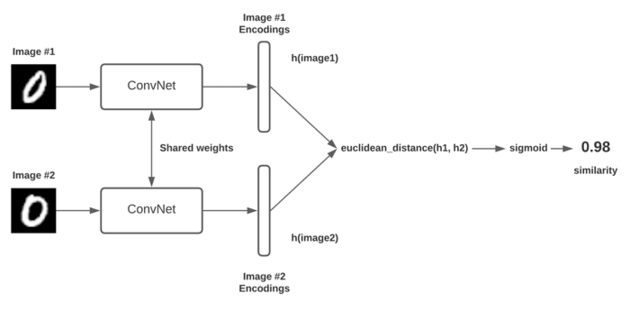
\includegraphics[width=1\columnwidth]{figures/siamese.png}
	\caption{A sziámi háló architektúra.}
	\label{fig:siamese}
\end{figure}

A \ref{fig:siamese}. ábrán láthatjuk a sziámi háló működését. A sziámi hálónak két bemenete van, az egyes bemenetekhez külön külön alháló tartozik. Az első alháló megkapja a bemenő képet, és miután az áthaladt a konvolúciós rétegeken létrehoz egy jellemzővektort (angolul feature vector vagy encoding), ami csökkentett dimenziójú a bemeneti képhez képest. A második alháló ami ugyanolyan súlyokkal dolgozik és egy különböző képet kap a bemenetén. Ezt követően a két jellemzővektorunk van, rendre $\mathbf{p} = f(\mathbf{x_1})$ és $\mathbf{q} = f(\mathbf{x_2})$. A két jellemzővektort ezután valamiyen távolság metrika szerint összevethető, ami alapján meghatározzuk a hasonlóságot. A sziámi háló célja egy olyan metrika megtanulása, amely közel azonosnak tekinthető bemeneti képekre nagy hasonlóságot ad, míg az eltérő képekre kis hasonlóságot kapunk.

A jellemzővektorok összehasonlításához többféle távolság metrikát is használhatunk. Ezek közül leggyakrabban a használt metrika a két vektor euklideszi távolsága (ami megegyezik jellemzővektorok külömbségének $L2$ normájával), ami egyszerűen kiszámolható az alábbi módon n dimenziós esetben \cite{tabak2014geometry}:

% On the n-dimensional Euclidean space {\displaystyle \mathbb {R} ^{n},}{\displaystyle \mathbb {R} ^{n},} the intuitive notion of length of the vector x = (x1, x2, ..., xn) is captured by the formula

\[ d(\mathbf{p},\mathbf{q}) = \lVert \mathbf{p} - \mathbf{q} \rVert_2 = \sqrt{(p_1 - q_1)^2 + (p_2 - q_2)^2 + \dots + (p_n - q_n)^2}\]

Ahol $\mathbf{p} = (p_1, p_2, \dots, p_n)$ és $\mathbf{q} = (q_1, q_2, \dots, q_n)$ 

\begin{figure}[h]
	\centering
	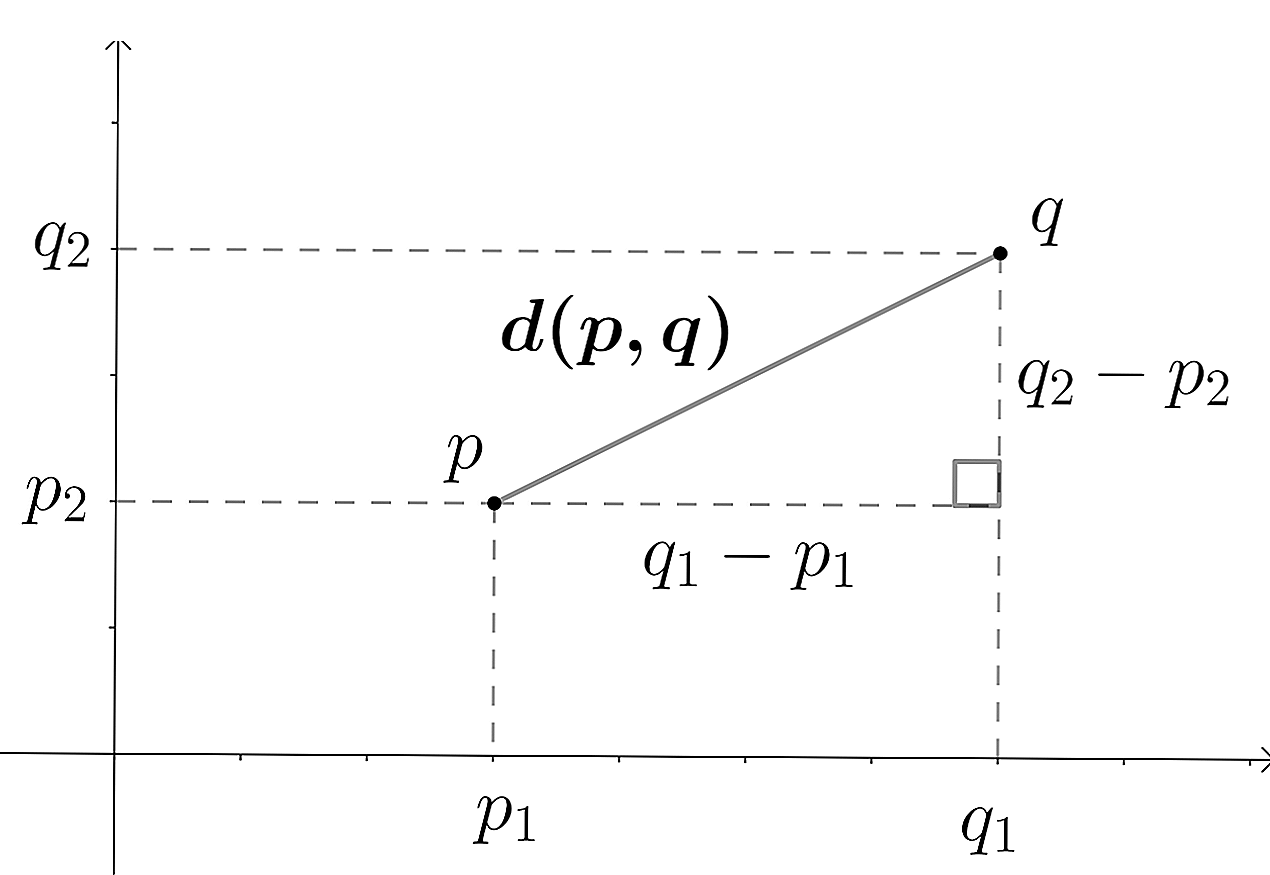
\includegraphics[width=0.65\columnwidth]{figures/euklidesz.png}
	\caption{Két pont euklideszi távolsága 2D esetben}
	\label{fig:eukl}
\end{figure}

\subsubsection{Sziámi hálók tanítása}

Mivel a sziámi hálózatok képzése általában páros tanulással (angolul pairwise learning) jár, a keresztentropia veszteség ebben az esetben nem használható, főként két veszteségfüggvényt használnak ezeknek a sziámi hálózatoknak a betanítására: a hármas veszteségfüggvényt (triplet loss) és a konsztratív veszteségfüggvényt (constrative loss).

A hármas veszteség lényege, tanítás során három sziámi háló bemenetére három különböző képet adunk. A három képből az elsőt referenciának nevezik (anchor), a másodikat pozitív példának, amely a referenciához nagyon hasonló kép, a harmadikat pedig negatív példának, amely a referenciától jelentősen eltérő kép. A tanítás során a neurális háló paramétereit úgy módosítjuk, hogy a referencia bemenetből és a pozitív bemenetből kinyert jellemzővektorok távolsága minimalizálva legyen, míg a referencia bemenetből és a negatív bemenetből kinyert vektorok távolsága minimalizálva legyen \cite{hoffer2015triplet}.

% A hármas veszteség egy veszteségfüggvény, ahol az alapvonal (horgony) bemenetét pozitív (truthy) bemenettel és negatív (hamis) bemenettel hasonlítják össze. Az alapvonali (horgony) bemenet és a pozitív (igaz) bemenet közötti távolság minimálisra csökken, az alapvonali (horgony) bemenet és a negatív (hamis) bemenet közötti távolság pedig maximalizálva van. \cite{facenet2015}

% Triplet loss is a loss function where a baseline (anchor) input is compared to a positive (truthy) input and a negative (falsy) input. The distance from the baseline (anchor) input to the positive (truthy) input is minimized, and the distance from the baseline (anchor) input to the negative (falsy) input is maximized. \cite{facenet2015}

\[ \mathcal{L}(A,P,N) = max \left( \lVert f(A) - f(P)) \rVert_2 - \lVert f(A) - f(N) \rVert_2 + \alpha, 0 \right) \]

A fenti egyenletben szereplő $f(A), f(P), f(N)$ a jellemzővektorokat jelöli (sorra referencia, pozitív és negatív bemenetekre), míg az $\alpha$ paraméterrel ``megnyújtható'' a hasonló és eltérő párok távolsága. 

% In the above equation, alpha is a margin term used to “stretch” the distance differences between similar and dissimilar pairs in the triplet, fa, fa, fn are the feature embeddings for the anchor, positive and negative images.

Kellő mennyiségű tanító kép és megfelelően választott kép hármasok használata esetén elérhető, hogy a neurális háló megtanuljon általánosítani, vagyis olyan képekből is megfelelő jellemzővektorokat hozzon létre, amelyeket nem használtunk a tanítás során. 

% Az  arcfelismeréshez  használt  arclenyomat  vektorokat  létrehozó  sziámi  hálók tanítására többek között egy úgynevezett „triplet loss” veszteségfüggvényt alkottak meg a kutatók. E veszteségfüggvény használatának lényege az, hogy tanítás során három sziámi háló bemenetére mindig három különböző arcképet adunk. E három arcképből az elsőt  kinevezzük  referenciának,  a  másodikat  pozitív  példának  (mely  ugyanannak  az embernek az arcát ábrázolja, mint a referencia), a harmadikat pedig negatív példának (mely másik ember arcát ábrázolja). A tanítás során a neurális háló paramétereit úgy módosítjuk, hogy olyan arclenyomat vektorokat állítson elő a bemeneti képekből, hogy a referencia és a pozitív példáról készült arclenyomatok távolsága minél kisebb, míg a referencia és a negatív példa közötti távolság minél nagyobb legyen. Kellő mennyiségű tanító kép és megfelelően választott kép hármasok használata esetén elérhető, hogy a neurális  háló  megtanuljon  általánosítani,  vagyis  olyan  arcképekről  is  megfelelő arclenyomat vektorokat hozzon létre, amelyeket nem használtunk a tanítás során. 
%~~~~~~~~~~~~~~~~~~~~~~~~~~~~~~~~~

% Contrastive Loss: is a popular loss function used highly nowadays, It is a distance-based loss as opposed to more conventional error-prediction losses. This loss is used to learn embeddings in which two similar points have a low Euclidean distance and two dissimilar points have a large Euclidean distance.

% So when A and B are the same person, we will have a label y equal to 1 and when A and B are different,y is equal to zero.

% By using contrastive loss, we bring positive pairs together and negative pairs apart. But using this loss function we cannot learn ranking which means we are not able to say how much two pairs are similar to each other, we shall see how to do this in the next section.

% When using contrastive loss we were only able to differentiate between similar % and different images but when we use triplet loss we can also find out which % image is more similar when compared with other images. In other words, the % network learns ranking when trained using triplet loss.

A sziámi hálók tanítása során gyakran alkalmazzák még a konsztratív veszteségfüggvény is. Ez egy távolság alapú veszteségfüggvény, nem a becsült kimenet és az elvárt kimenet külömbségéből származtatott. A konsztratív veszteségfüggvényt főleg embeddingek tanulására használják, azzal a céllal, hogy két hasonló adatpontból származtatott embedding távolsága kicsi legyen, eltérő adatokból származtatott embeddingek távolsága pedig nagy legyen. 

% TODO ezt double check h helyes-e
\[ \mathcal{L}(A,B) = y \lVert f(A) - f(B)\rVert_2^2 + (1-y) max\left(0,m - \lVert f(A) - f(B) \rVert_2^2 \right) \]

Abban az esetben, ha A és B két ugyanaz a kép, akkor a háló kimenete ($y$) 1 lesz, míg mikor A és B eltér, akkor a háló kimenete 0 lesz. 

%----------------------------------------------------------------------------
\section{Probléma bemutatása}
%----------------------------------------------------------------------------


%----------------------------------------------------------------------------
\section{Arclenyomatok adatvédelmi elemzése}
\label{sec:4}

%--------------------------------------------------------------------------------------------------
\subsection{Támadó modellezése} % 1 oldal
\label{sec:tamado}
% - Támadómodell bemutatás (copy ábra Gábortól, lényeget leír)
% - Jelenlegi arcfelismerő rendszerek sebezhetősége, hogyan férhet hozzá
% - Feltételezzük, hogy a támadó interneten elérhető datasetekhez hozzájut ami alapján betanít classifiert és ezt használva tud kinyerni adatot. Következő fejezetben erre mutatunk példát hogyan lehetséges

A következőkben az arcfelismerő rendszerek sebezhetőségét fogom elemezni. Az arcfelismerő rendszerek általános működését a \ref{sec:problem}. fejezetben korábban bemutattam. Az adatvédelmi elemzéshez szükséges definiálnom egy támadó modellt. Tegyük fel, hogy egy cégnél alkalmaznak arcfelismerő rendszert a dolgozók azonosítására. Az épület számos helyisége le van fedve CCTV térfigyelő kamerákkal, amelyek egy központi arcfelismerő rendszernek továbbítják a felvételeket. Új dolgozó regisztrációja során az arcfelismerő rendszer néhány felvétel alapján kiszámolja a dolgozó arcát legjobban leíró arclenyomatát, amit egy központi szerveren tárol. Miután a dolgozó arclenyomata szerepel az adatbázisban, a térfigyelő kamera felvételek alapján lehetséges őt azonosítani. Egy ilyen arcfelismerő rendszernek a főbb részei: 

\begin{enumerate}
	\item \textbf{Kamera rendszer}: amely a nyers képkockákat továbbítja az adatfeldolgozó egységnek
	\item \textbf{Jellemző kinyerő}: amely az egyes képkockákon végzi a gyorsan lefuttatható arcdetektálást. Ha sikeresen talál emberi arcot az egyik képkockán, arra elvégzi az arc geometriai transzformációját, majd az arcból kinyeri az arclenyomatot.
	\item \textbf{Adatbázis}: Az ismert, címkézett arclenyomatok tárolására szolgál.
	\item \textbf{Összevető}: A kinyert arclenyomatot összehasonlítja az adatbázisban tárolt dolgozók arclenyomataival, majd azokon valamilyen távolság (pl: Euklideszi távolság) metrika alapján megállapítja a legvalószínűbb találatot. Ha a legkisebb távolság egy bizonyos küszöbértéknél kisebb, akkor a dolgozót sikeresen azonosította, ellenkező esetben ismeretlen személynek nyilvánítja.
\end{enumerate}

Míg az ilyen arcfelismerő rendszer több módon is támadható, a dolgozatom során azzal az esettel foglalkozom, hogy a rosszindulatú fél valamilyen módon hozzáférést nyer az arclenyomat adathalmazhoz, ami lehet egy belső alkalmazott aki kiszivárogtatja az adatbázist, vagy akár egy külső támadó, például hacker aki sikeresen feltöri rendszert. Előfordulhat, hogy a támadó az adatbázisnak egy kisebb részéhez fér hozzá, de dolgozatom során a legerősebb támadót feltételezem, aki a teljes adatbázishoz hozzáfér, illetve feltételezem, hogy az arclenyomatok titkosítás nélkül vannak tárolva a szerveren.

\begin{figure}[ht]
	\centering
	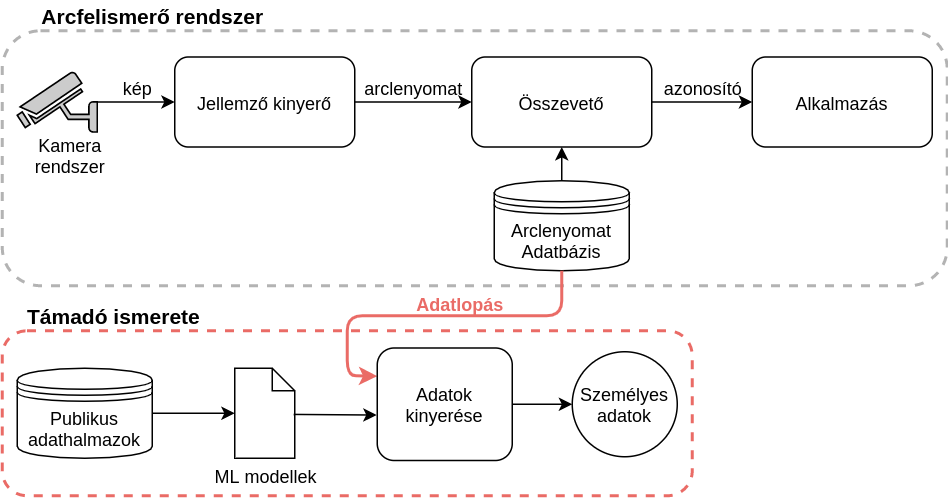
\includegraphics[width=1\columnwidth]{figures/attacker_model.png}
	\caption{Az arcfelismerő rendszer és a támadó modellezése.}
	\label{fig:attacker}
\end{figure}

A támadó modellezését a \ref{fig:attacker}. ábra mutatja be. Miután a támadó valamilyen módon hozzáférést szerzett a központi szerverhez, amin az arclenyomatok vannak tárolva, elképzelhető, hogy képes lesz az arclenyomatokból személyes adatokat kinyerni az adatalanyokról. Személyes adatnak minősül bármilyen adat, ha közvetlenül beazonosítható általa az érintett személy (közvetlen azonosítók), vagy ha közvetetten (kvázi-azonosítók) \cite{GDPR2018}. Személyes adat lehet például a személy demográfiai adatai, mint például a személy életkora, a neme, vagy a rassza. 

Feltételezhetjük, hogy a támadó a személyes adatok kinyeréséhez egy saját fejlesztésű algoritmust használ, ami lehet például egy gépi tanulási modell is. Ha a támadó képes megfelelően nagy valószínűséggel, megbízható módon kinyerni a személyes adatokat, akkor a támadó feltételezheti, hogy a kinyert adatok valósak. A sikeresen kinyert adatokat majd saját célból fel tudja használni a támadó, például újraazonosításos támadáshoz. A személyes adatok kiszivárgásának adatvédelmi kockázatait a \ref{sec:adatvedelmi_elemz}. fejezetben fejtem ki bővebben.

A kérdés az, hogy milyen eljárással lehetséges egy arclenyomatból kinyerni az adatalany érzékeny információit? A munkám során erre a kérdésre kerestem választ. Feltételezésem az volt, hogy az interneten ingyenesen, publikusan elérhető emberi arcokról készült fotókból összeállítható egy nagy méretű adathalmaz, amihez rendelkezésre állnak a fotón látható valamennyi személy demográfiai adatai, például a pontos vagy becsült életkora, neme és rassza, vagy bármilyen adat ami fotó alapján ember által megadható, és később segíthet az illető azonosításában. Ha sikerül egy ilyen adathalmazt összeállítani, akkor az arcképek alapján az arcfelismerő rendszer működéséhez hasonlóan minden arcképről generálhatunk arclenyomatokat. Ezt követően rendelkezünk az arclenyomatokkal, és a hozzájuk tartozó címkékkel.

Miután megvan az arclenyomat adathalmaz, az alapján képesek vagyunk betanítani egy gépi tanulási modellt, ami az arclenyomatok és a hozzájuk tartozó címkék alapján képes tanulni. A betanítás után a modell használható arra, hogy új, nem látott arclenyomat mintákra becslést adjon. Visszatérve a támadóhoz, ha a támadó rendelkezik egy előre betanított gépi tanulási modellel, azt felhasználhatja arra, hogy a szerverről szerzett arclenyomat adatbázisból érzékeny adatokat nyerjen ki. 

A támadó sikerességének feltétele az, hogy képes hozzáférni a szerveren tárolt arclenyomatokhoz, illetve az, hogy a gépi tanulási modellje milyen megbízhatósággal képes becslést hozni a személyes adatokra. A két feltétel közül a másodikkal foglalkozom a továbbiakban. Azt vizsgáltam, hogy modern tanuló algoritmusokkal milyen eredmény érhető el.

%--------------------------------------------------------------------------------------------------
\subsection{Adathalmazok} % 3-4 oldal

Első lépésként szükségem volt egy megfelelően felcímkézett arclenyomat adathalmazra. Ezt az adathalmazt használom fel arra, hogy az alapján tanítsak be gépi tanulási modelleket, amelyek majd képesek becslést adni személyes adatokra. Egy-egy modell csak egy személyes adatra tud becslést adni, ezért több modellre van szükség. Célom az volt, hogy személyes adatok közül az illető életkorát, nemét és rasszát becsüljem meg. Ehhez szükséges tanító mintakészlet, amiben az életkor, nem és rassz meg van címkézve. Elvárás volt még az is, az arclenyomat adathalmazban minden személynek saját azonosító címkéje legyen, illetve lehetőleg minél több arclenyomat tartozzon egy-egy személyhez. Erre azért van szükség, mert az arclenyomatokon vizsgáltam az identifikációs modell teljesítőképességét is. 

Mivel a feladatból adódóan az adathalmazzal szemben támasztott elvárások eléggé specifikusak, ezért szükség volt saját adathalmaz létrehozására. Azért, hogy meggyorsítsam a munkámat, kiindulásnak kerestem olyan online elérhető, arcképeket tartalmazó adathalmazt, ami már előre fel van címkézve. Ha létezik egy megfelelő arckép adathalmaz, akkor a képekből egyesével kinyerhetőek az arclenyomat vektorok. Az arckép adathalmazzal szemben az elvárások a következők:
\begin{itemize}
	\item Lehetőleg kutatási célra lettek létrehozva, az enyémhez hasonló feladatra. Ennek megfelelően az arcképek már előre vannak készítve a feldolgozáshoz (pl. arc kivágása a képből).
	\item Az adathalmaznak megfelelően nagynak kell lennie ahhoz, hogy gépi tanulási modellt sikeresen be lehessen tanítani róla.
	\item Egy emberről lehetőleg minél több kép legyen ahhoz, hogy a generált arclenyomatok alapján identifikáció jól működjön. Minél több képünk van egy illetőről, annál biztosabban lehet meghatározni az ember arcát legjobban leíró arclenyomatot.
	\item A képek megfelelő demográfiai adatokkal vannak címkézve. Esetemben a szükséges címkék: az életkor, nem és a rassz.
\end{itemize}

Nehéz olyan adathalmazt találni, amiben mindhárom számunkra fontos demográfiai adat szerepel. Több arckép adathalmaz jónak tűnt elsőre, de az elvárások közül nem felelt meg egynek. Néhány ilyen adathalmaz amivel foglalkoztam: Labled Faces in the Wild \cite{labledfacesinthewild2008}, Face Image Project \cite{faceimageproject2014}, CelebA \cite{celebA2015}. A FairFace \cite{fairface2021} egy viszonylag új adathalmaz, ami nagyon ígéretesnek tűnt, mert mindhárom demográfiai adatot tartalmazza, és az egyes osztályok aránya kiegyensúlyozott, viszont nem tartalmaz identifikációs címkét.

Végül nem sikerült olyan adathalmazt találnom ami minden kritériumnak megfelel, ezért két külön adathalmazt használtam fel. Az egyik a VGGFace2 \cite{vggface22018} amit rassz és nem becslésére használtam fel, a másik pedig az IMDB-WIKI dataset \cite{imdbwiki2018}, amit életkor becsléshez használtam fel. A két választott arckép adathalmazt szükség volt feldolgozni ahhoz, hogy azokból gépi tanulási modellt lehessen tanítani. A feldolgozás menetét mutatom be a következő részekben.

\subsubsection*{VGGFace2 adathalmaz}

Jelenleg az egyik legnagyobb publikusan elérhető, kutatási célra készült arckép adathalmaz a VGGFace2. Az adathalmaz 3,31 millió arcképet tartalmaz mindössze 9131 emberről, átlagosan 362,6 kép mindenkiről. A képeket a Google képkeresőjével gyűjtötték össze. Az adathalmaz képein sokféle ember szerepel, eltérő demográfiai adatokkal és eltérő szakmával (pl. vannak színészek, sportolók, politikusok). A képeken látható emberek többféle pózban láthatóak, sokféle megvilágításban. Az összegyűjtött képeket automatikusan és manuálisan is szűrték.

A VGGFace2 alapból nem tartalmaz rassz címkéket, viszont a Salernói Egyetem MIVIA kutatócsoportja manuálisan felcímkézte az adathalmazt rassz címkékkel, és a munkájukat publikusan elérhetővé tették VMER névvel \cite{vmer2020}. A VMER-rel kiegészítve a VGGFace2 címkéit, így már van rassz, nem és identifikációs címke is az összes mintához.

Az arcképeket egyesével dolgozza fel egy script, ami az arcképekből kinyeri az arclenyomatokat. Ehhez a face\_recognition Python könyvtárat \cite{face_recognition} használtam fel, ami a \ref{sec:problem}. fejezetben taglalt módon találja meg, és alakítja át a képen látható arcokat arclenyomattá. Az arclenyomatok kinyeréséhez a dlib-et \cite{dlib2009} használja, így a kapott arclenyomatok 128 dimenziós lebegőpontos vektorok lesznek. Az adathalmazban előfordulnak olyan képek, ahol több ember arca is látható, (például a háttérben elsétál valaki). Ez problémás, mivel ilyenkor nem egyértelmű, hogy a képen látható melyik archoz tartozik az annotáció. E miatt a scriptem csak olyan képekkel foglalkozott, ahol pontosan egy arcot sikerült azonosítani. A script-ből egy függvény látható a \ref{lst:get_encoding}. kódrészleten.

\begin{lstlisting}[language=python, caption={Arclenyomat vektorok kinyerése.}, label=lst:get_encoding]
def get_encoding(filepath):
  # kep beolvasasa
  image = face_recognition.load_image_file(filepath) 
  # arcok detektalasa 
  face_locations = face_recognition.face_locations(image,
    number_of_times_to_upsample=1, model="cnn")
  if (len(face_locations) == 1): 
    # arclenyomat vektor
    return np.array(face_recognition.face_encodings(image,face_locations))[1]
  return None
\end{lstlisting}


Mivel 3,3 millió arcképet kellett feldolgozni, a Python scriptet Google Colab-en futtattam, aminek az az előnye, hogy ingyenesen lehet használni korszerű GPU-kat, illetve az adathalmaz feldarabolásával párhuzamosan több session-t is lehet futtatni, jelentősen felgyorsítja a képek feldolgozását.

A következő lépés az adathalmaz tisztítása volt, azaz kiszűrni azokat a képeket, amelyek valamilyen okból rossz minőségűek (például távoli fotó, rossz fényviszony vagy fura szögből készült a kép), vagy az illető a többi képhez képest nagyon eltérően néz ki. Az arclenyomatok szűréséhez minden személyhez kiszámítottam az átlagos arclenyomatot (centroid), és a centroidtól vett távolság alapján a túl nagy távolságra lévő arclenyomatokat szűrtem az adathalmazból. 

A feldolgozás és szűrés után kapott adathalmaz közel 3 millió arclenyomatot tartalmaz. Minden arclenyomathoz tartozik egy ID címke ami azonosítja az képen látható személyt. Egy ID-hoz legalább 50 arclenyomat tartozik. E mellett van még nem címke (férfi, nő), és rassz címke (African American, East Asian, Caucasian Latin, Asian Indian). Ekkor probléma volt az, hogy az egyes osztályokhoz sokkal több minta tartozott mint más osztályokhoz. A leggyakoribb a fehér férfiak aránya volt, míg a legritkább az afroamerikai nők. Az osztályok arányát a \ref{fig:vgg_imba}. ábra mutatja be.

\begin{figure}[ht]
	\centering
	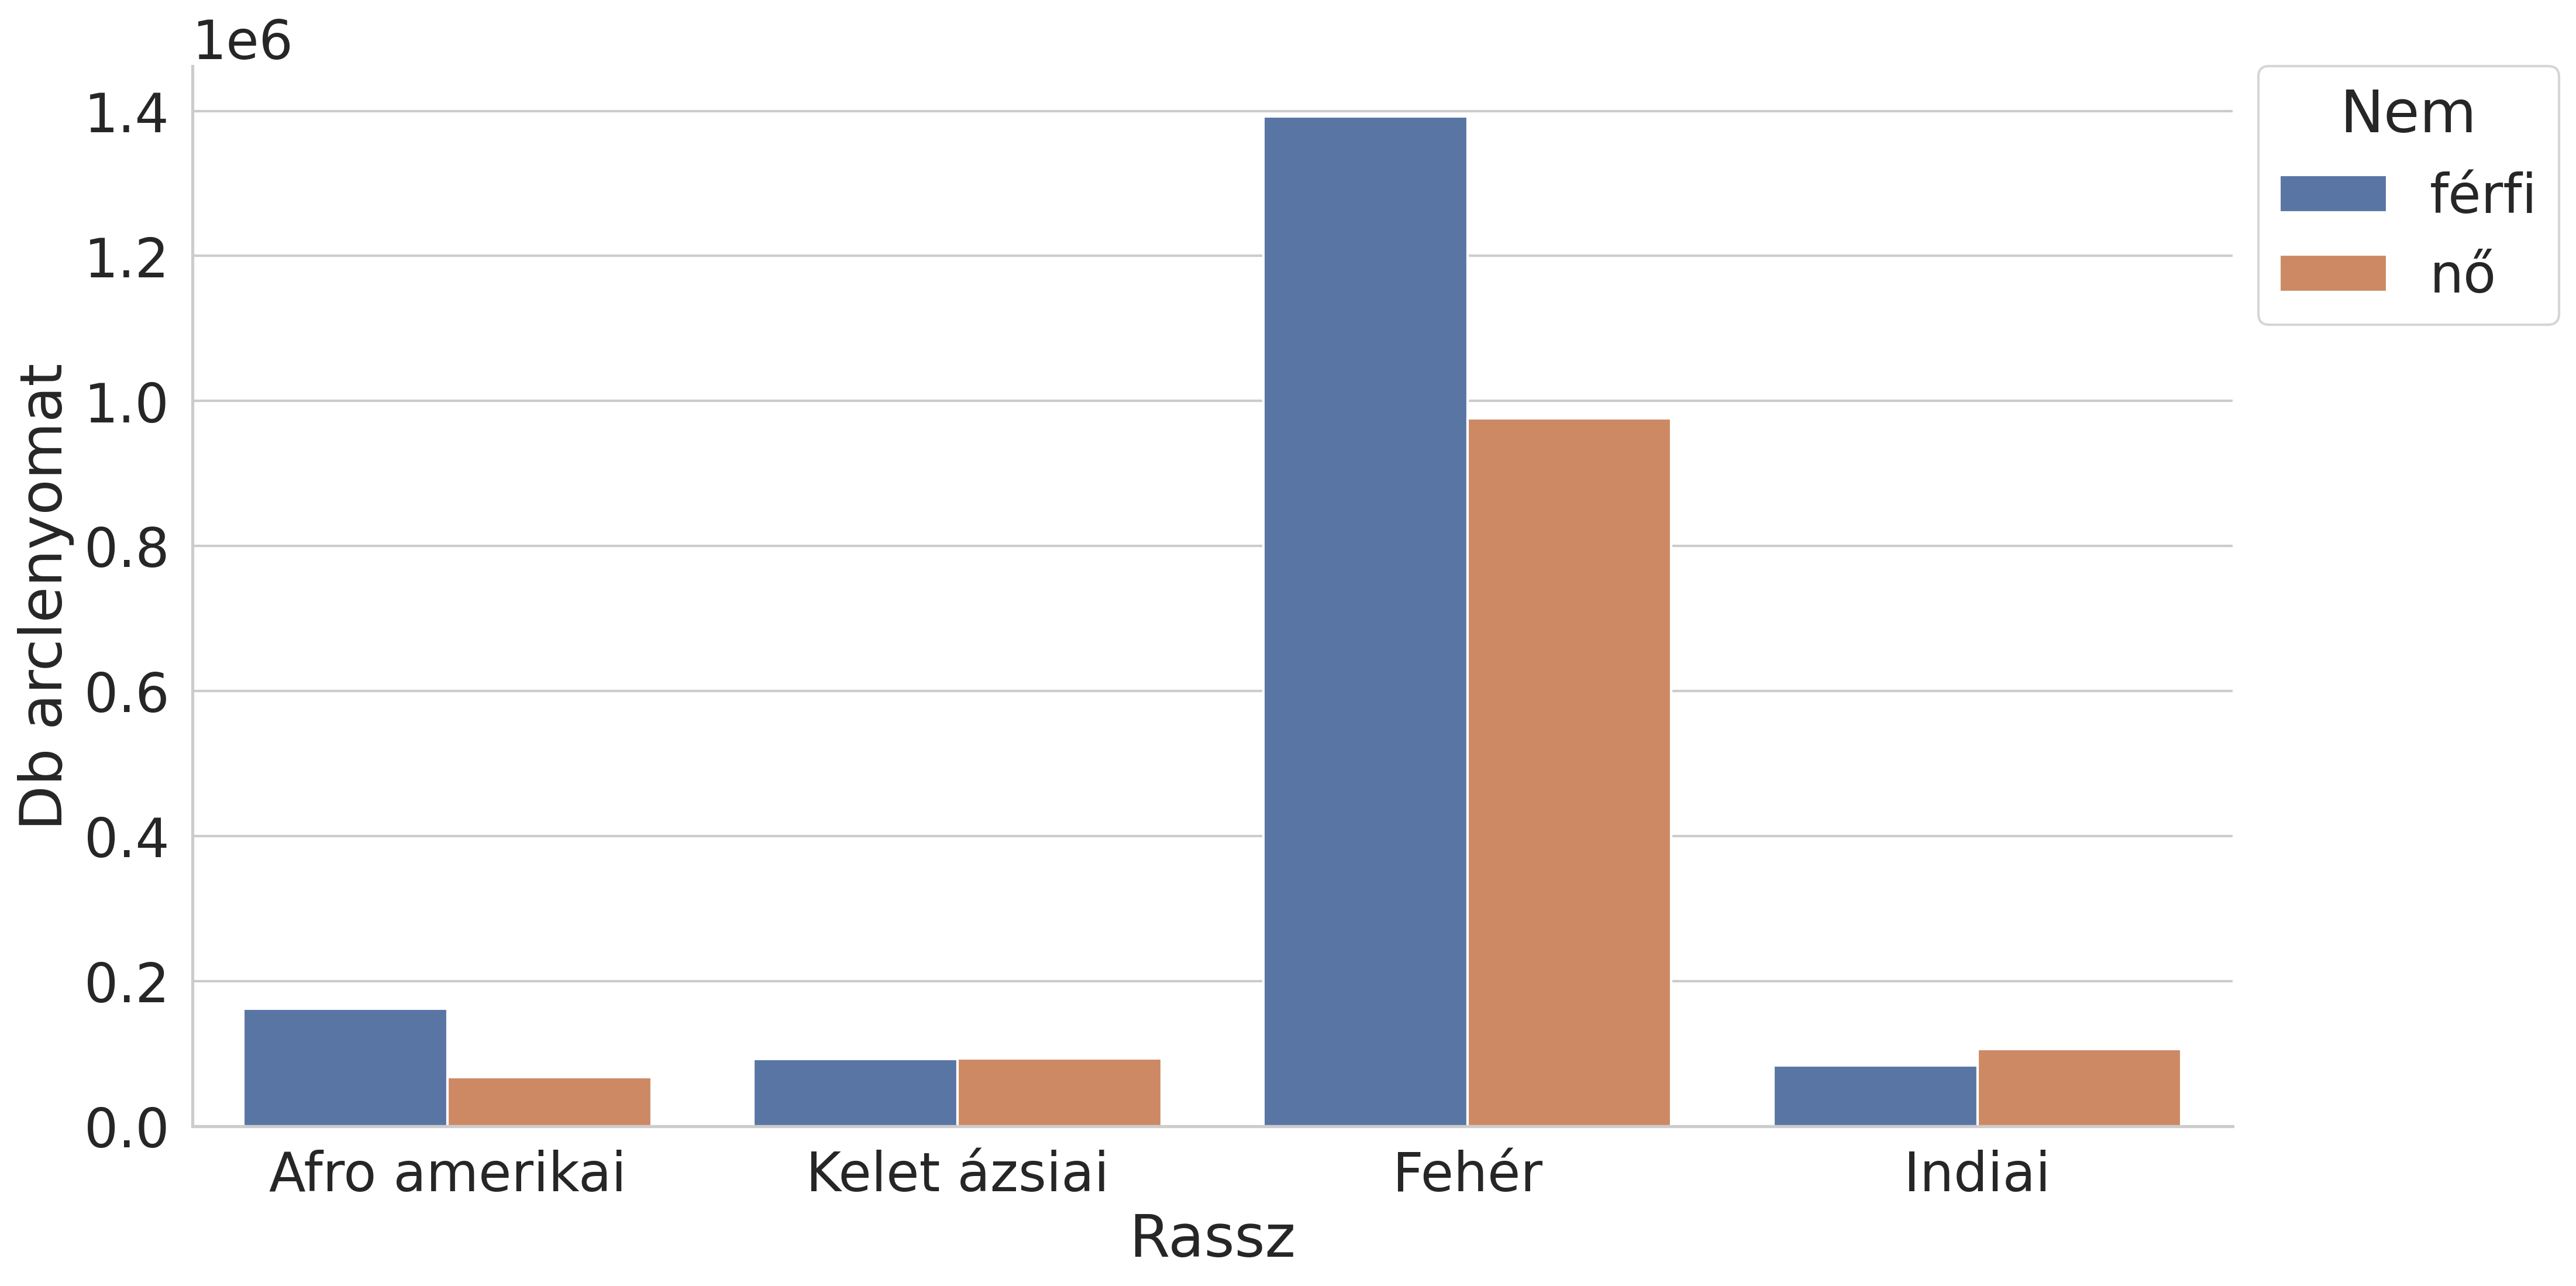
\includegraphics[width=1\columnwidth]{figures/VGG_imba.png}
	\caption{Osztályok aránya az arclenyomat adathalmazban.}
	\label{fig:vgg_imba}
\end{figure}

Az osztályok eloszlásának aránytalansága problémát jelent az osztályozó modellek tanításakor, ezért szükséges volt az adathalmazt kiegyensúlyozni. Az adathalmaz kiegyensúlyozása minták eltávolításával érhető el. Legkevesebb kép az afroamerikai nőkről van az adathalmazban, ezért ehhez mérten szűkítettem a többi csoportot. Az embeddingek kivételénél fontos volt, hogy továbbra is legalább 50 kép maradjon minden személyről, ezért nem véletlenszerűen vettem ki a képeket, hanem ID-k alapján csoportosítva. Az egyes demográfiai csoportoknál kilistáztam az oda tartozó ID-kat, és egyes ID-khoz tartozó képek számát. Az ID-kat képszám szerint csökkenő sorrendben távolítottam el, amíg a csoport meg nem közelítette a szükséges méretet. Ezzel a módszerrel sikerült elérni, hogy minden rassz-nem párhoz ugyanannyi ember tartozott. A kiegyensúlyozott után az osztályok eloszlása a \ref{fig:vgg_ba}. ábrán látható.

\begin{figure}[ht]
	\centering
	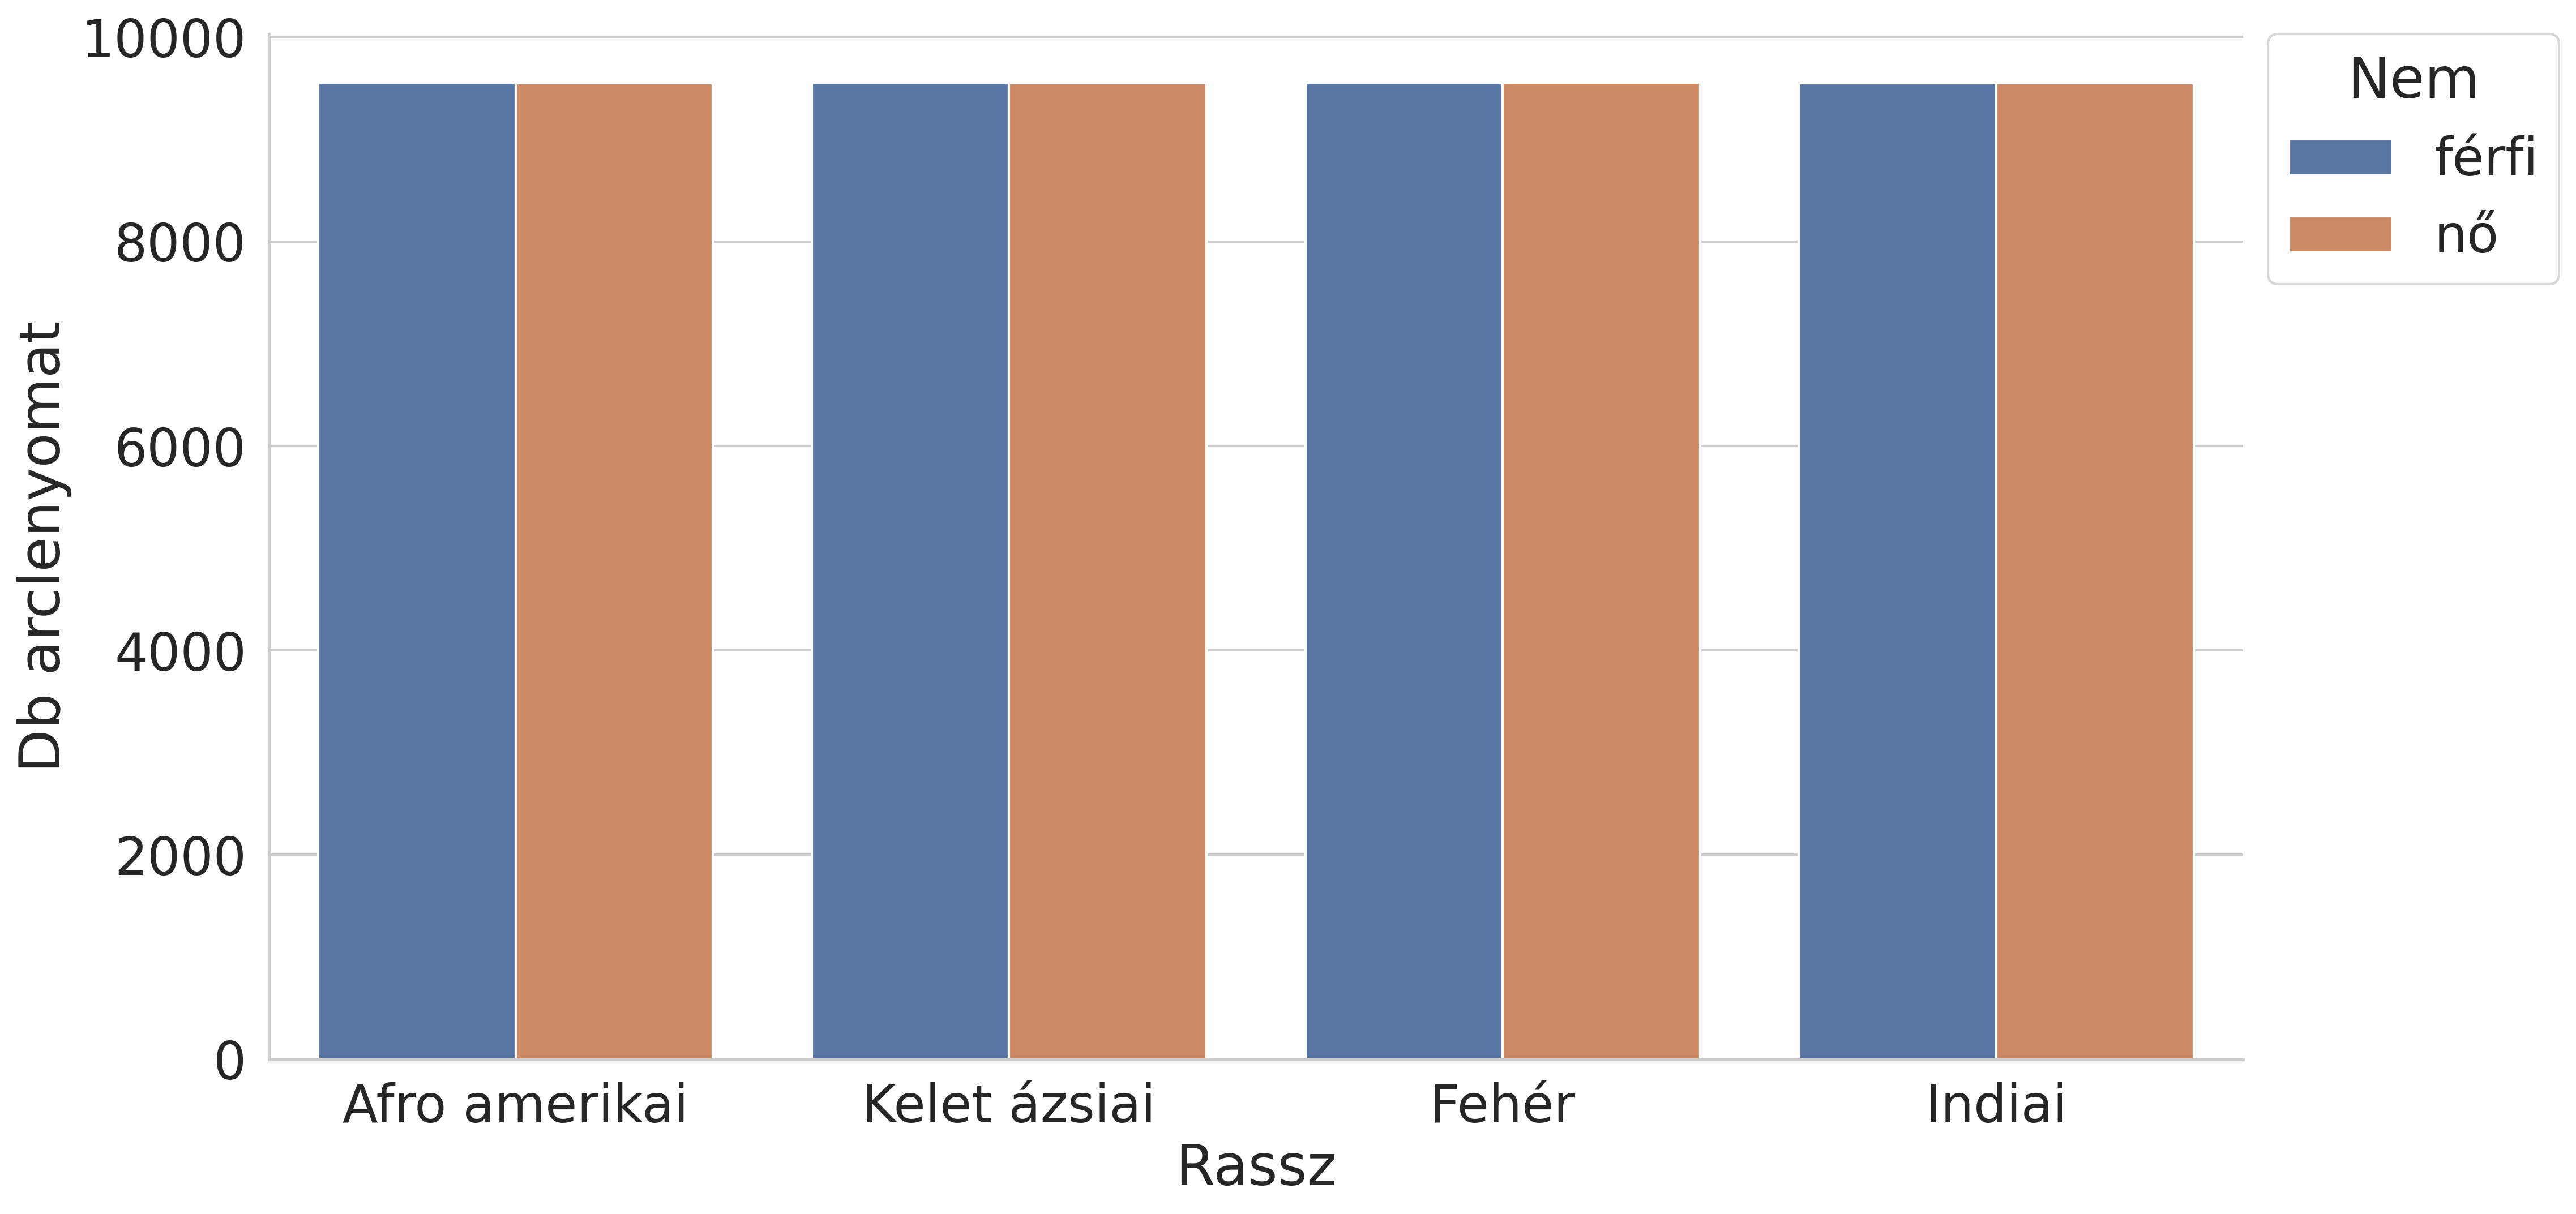
\includegraphics[width=1\columnwidth]{figures/VGG_balanced.png}
	\caption{Osztályok aránya az kiegyensúlyozás után.}
	\label{fig:vgg_ba}
\end{figure}

Az eredeti 3,3 millió képből végül 76410 arclenyomat készült, ami továbbra megfelelő méretű adathalmaznak tekinthető. Ez elegendően nagy ahhoz, hogy ez alapján osztályozó modelleket lehessen rajtuk betanítani.

\subsubsection*{IMDB-WIKI adathalmaz}

Mivel a VGGFace2 adathalmaz nem tartalmaz életkor címkét, ezért tovább folytattam a keresést. Választásom az IMDB-WIKI \cite{imdbwiki2018} adathalmazra esett. Ez az egyik legnagyobb, nyilvánosan elérhető arckép adathalmaz, ami tartalmaz azonosító címkét, nemet és életkort is. Az adathalmaz két részből áll: IMDB filmekről és filmszínészekből álló adatbázisból kinyert fotókból, illetve a Wikipédiáról szerzett fotókból. Sajnos a Wikipédiáról szerzett képekhez nem tartozik azonosító címke, így csak az IMDB-ről szerzett fotókat használtam fel.

Az IMDB-WIKI adathalmaz képekből, és hozzájuk tartozó címkékből áll. A címkék egy metadata fileban találhatóak, ami többek között tartalmazza a képen látható személy nevét, nemét, a születési dátumát, illetve azt, hogy mikor készült a fotó. A életkort a képen látható személy születési dátumából, és a kép keletkezésének dátuma alapján lehet kiszámolni. A képek jelentős része csoportkép, azaz több arc is látható rajtuk. A képek közül csak azokat használtam fel, ahol pontosan egy arcot lehetett detektálni. Továbbá, kiválasztottam azokat az azonosítókat, amihez legalább 30 fotó tartozik.

A weboldalról letölthetőek az eredeti, teljes méretű képek, illetve a már megvágott csak arcokat tartalmazó képek is. A képeken az arcok középre vannak rendezve 40\%-os ráhagyással. A képek feldolgozásánál ezért levágtam ezt a 40\%-ot, így gyorsabb a feldolgozás és jelentősen több képen sikerült arcot detektálni. Az arcokhoz tartozó képeket a VGGFace2-nél bemutatott módszerrel alakítottam át arclenyomat vektorokká.

\begin{figure}[ht]
     \centering
     \begin{subfigure}[b]{0.42\columnwidth}
         \centering
         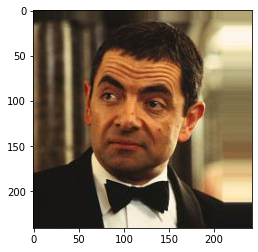
\includegraphics[width=1\columnwidth]{figures/mrbean.png}
     \end{subfigure}
     \begin{subfigure}[b]{0.42\columnwidth}
         \centering
         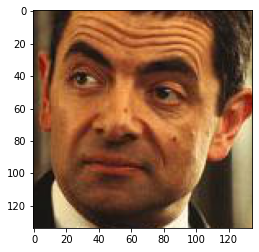
\includegraphics[width=1\columnwidth]{figures/mrbean_crop.png}
     \end{subfigure}
        \caption{Az eredeti és a megvágott kép}
\end{figure}


Az adathalmaz képeit vizsgálva azt tapasztaltam, hogy néhány fotón nem a címkének megfelelő személy szerepelt. A hibásan címkézett képek kiszűréséhez a már feldolgozott arclenyomat vektorokat használtam fel. Egy személyhez tartozó arclenyomat vektorok alapján kiszámítottam a vektorok súlypontját (centroidját), és ehhez mért Euklideszi távolságok alapján szűrtem ki a kiugró értékeket. Azt a határt, ami alatt elfogadta az arclenyomat vektor értékét 0,5-re állítottam be, ami viszonylag szigorúnak számít. Ezt az eljárást szemlélteti a \ref{lst:cent}. kódrészlet.

% \begin{minipage}{\columnwidth}
\begin{lstlisting}[language=python, caption={Arclenyomatok szűrése távolság alapján.}, label=lst:cent]
def filter(df, cutoff=0.5):
	encodings = df.iloc[:,4:].values  # egy szem(*@\color{codegreen}é@*)lyhez tartoz(*@\color{codegreen}ó@*) arclenyomatok
	centroid = np.mean(encodings, axis=0)  # s(*@\color{codegreen}ú@*)lypont sz(*@\color{codegreen}á@*)m(*@\color{codegreen}í@*)t(*@\color{codegreen}á@*)s
	distance = np.linalg.norm(encodings - centroid, axis=1)  # euklideszi t(*@\color{codegreen}á@*)vols(*@\color{codegreen}á@*)g
	return df.index[distance > cutoff]
\end{lstlisting}
% \end{minipage}

Feldolgozás után közel 90000 arclenyomat vektort kaptunk eredményül. Az adathalmazon belül a nemek aránya közel azonos, viszont az életkor eloszlása már kevésbé egyenletes (lásd: \ref{fig:agedist}. ábra). Mivel a képek az IMDB weboldalról lettek összegyűjtve, ezért főleg színészekről, filmrendezőkről vannak képek, akik tipikusan a 20-40-es életkor tartományba esnek. E miatt kiskorúakról és idős emberekről viszonylag kevés kép van az adathalmazban.

\begin{figure}[ht]
	\centering
	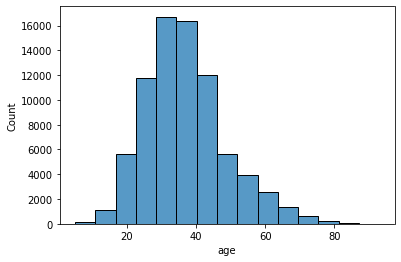
\includegraphics[width=0.7\columnwidth]{figures/IMDB_age_dist.png}
	\caption{IMDB adathalmazban az életkor eloszlása.}
	\label{fig:agedist}
\end{figure}

%--------------------------------------------------------------------------------------------------
\subsection{Modellek betanítása, eredmények} % 1 oldal RFC, 1-2 oldl eredmények
% - RFCről röviden, miért ezt választottam, 
% - Tanítás módszeréről (használt paraméterek, modell jellemzők, age hogy lett kezelve, ID hogy lett kezelve) 
% - Betanított modellek accuracy precision, recall, F1 score, Confusion matrix, ROC curve

% mi az az RFC, röviden

Az elkészült arclenyomat adathalmazok alapján betaníthatunk valamilyen osztályozó tanuló algoritmust, ami az arclenyomatok alapján becslést tud adni a személy demográfiai adataira. Gyakorlatban ehhez három osztályozó modellt tanítottam be: egyet a nem predikcióhoz, egyet a rasszhoz, egyet az életkorhoz. E mellett készítettem egy identifikációs modellt is, ami az arclenyomatok alapján azonosítani tudja a személyt. A három osztályozó modellhez döntési erdő struktúrát használtam.

Az egyik legalapvetőbb osztályozási algoritmus a döntési fa (angol szakirodalomban decision tree). A döntési fa tanítása során a tanító halmazt lépésenként két halmazra bontja szét az adatok különböző jellemzőire teljesülő vagy nem teljesülő feltétel alapján. Ezt a szétválasztó lépést majd sokszor megismétli, minden lépésnél egy-egy elágazást hoz létre. A feltételek alapján szétválogatott adatok így különböző osztályokba kerülnek. A döntési fák általánosítási képessége javítható, ha azokat egy szakértő együttes (ensemble) struktúrába rendezzük. Ekkor a tanító mintakészletre több, eltérően inicializált döntési fát tanítunk be, amik együttesen egy ``döntési erdőt'' képeznek. Ekkora egy bemeneti mintára a döntési erdő minden fája képez egy becslést, hogy melyik osztályba tartozik a minta. Az döntési erdő kimenete az az osztály lesz, amelyikre a legtöbb döntési fa szavazott. Az osztályozó modellekhez a Scikit-learn Python könyvtár döntési fa implementációját használtam. Ennek a modellnek az az előnye, hogy a használata egyszerű, mivel hiperparaméterek rögzítése nélkül is jó eredményeket lehet elérni.

\subsubsection*{Nem becslése}

A nem becslő osztályozó modell tanításához a VGGFace2 arclenyomat adathalmazt használtam fel. Az arclenyomatok $N\times128$ dimenziós mátrix formában vannak, a hozzájuk tartozó címkék $N\times1$ méretű vektorban, ahol $N$ az adathalmaz mintáinak száma. A teljes mintakészletet felosztottam tanító halmazra és teszt halmazra úgy, hogy a tanító halmaz a minták 70\%-át, a teszt halmaz a minták 30\%-át tartalmazza. A minták osztályozásához 100 döntési fából álló véletlen erdő modellt használtam. A modell betanítása után a pontosságát a teszt adathalmazon ellenőriztem. A teszt halmaz kb. 23000 mintából állt, amiből a modell csak 276 mintánál tévesztett. A modell jóságát a \ref{fig:conf_sex}. ábra mutatja, ahol az osztályozó igazságmátrixa látható. 

\begin{figure}[ht]
	\centering
	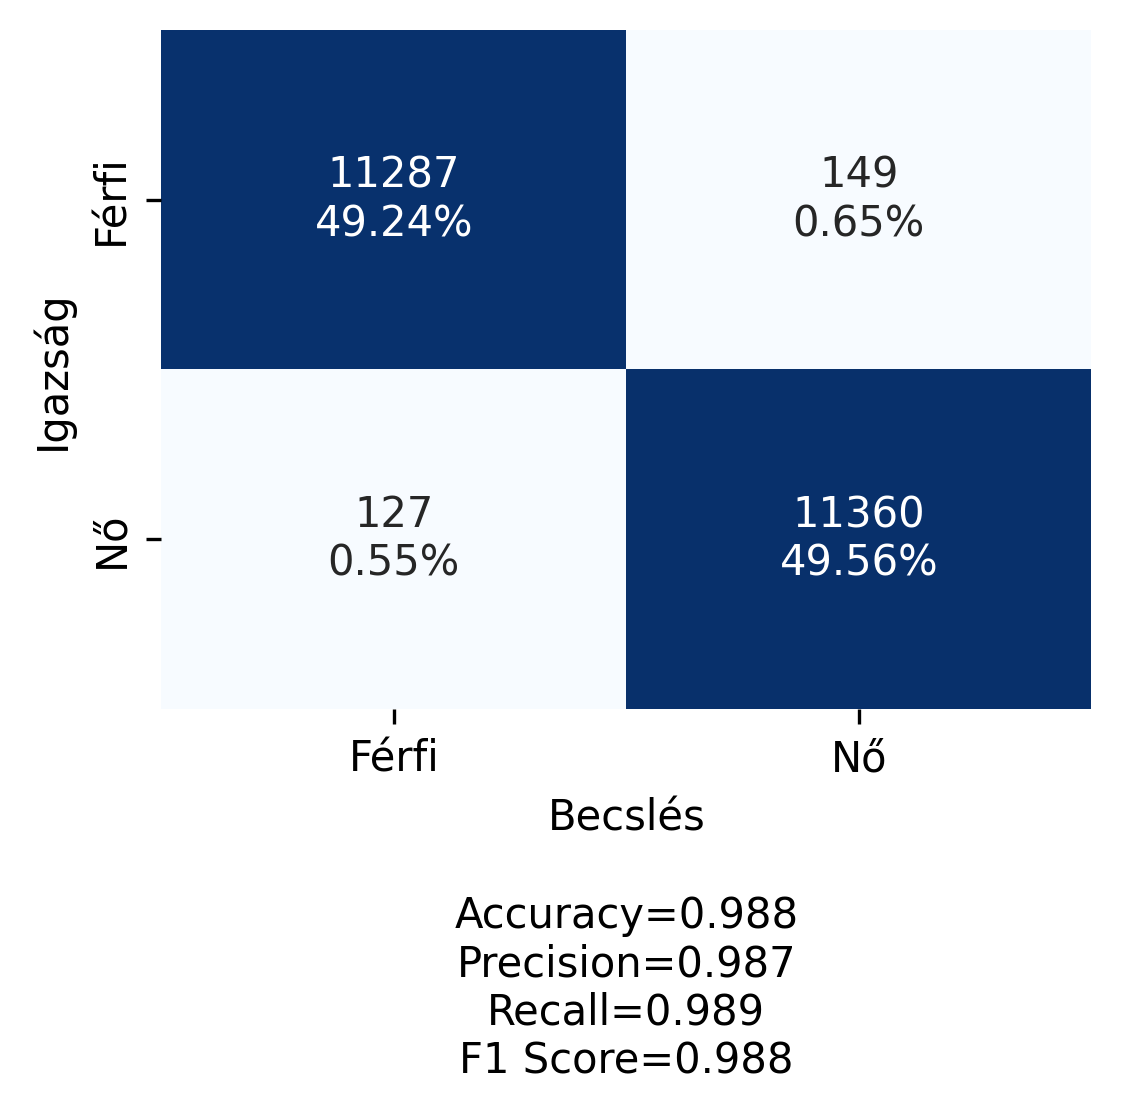
\includegraphics[width=0.5\columnwidth]{figures/conf_sex.png}
	\caption{A nemet osztályozó modell igazságmátrixa és pontossági metrikái.}
	\label{fig:conf_sex}
\end{figure}

\subsubsection*{Rassz becslése}
A rassz osztályozó modellt a nem osztályozóhoz hasonlóan tanítottam be, azzal a különbséggel, hogy itt bináris osztályozás helyett már 4 osztályunk van, ami nehezebb feladatnak számít. A négy osztály: afro amerikaiak, kelet ázsiaiak, fehérek, és indiaiak. A VGGFace2 adathalmaz kiegyensúlyozottságának köszönhetően itt is sikerült jó pontosságot elérni. A modell igazságmátrixát a \ref{fig:conf_race}. ábra mutatja be. A többosztályos osztályozó modell pontossági metrikáinak kiszámításához ``macro'' átlagoló módszert használtam.

\begin{figure}[ht]
	\centering
	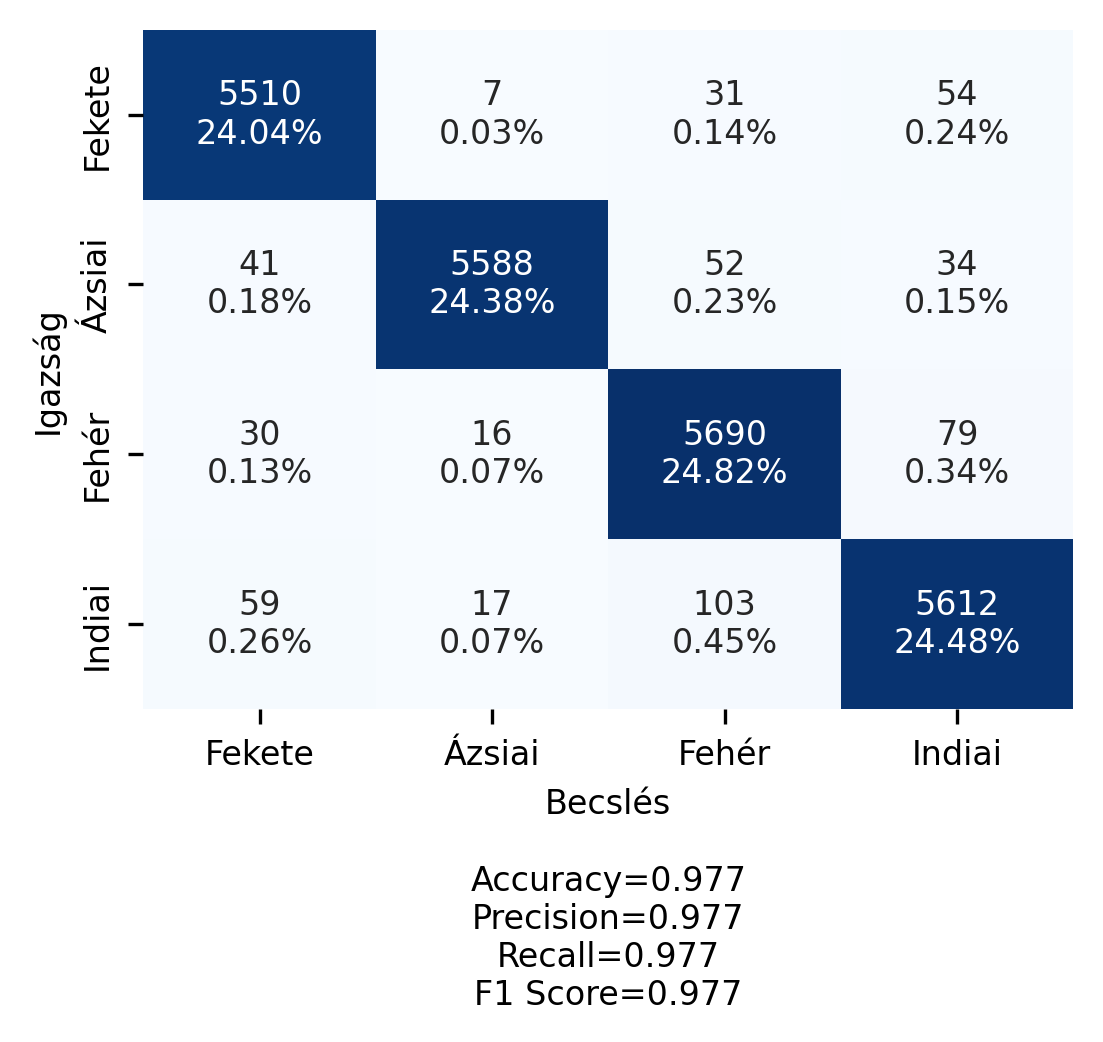
\includegraphics[width=0.7\columnwidth]{figures/conf_race.png}
	\caption{A rassz osztályozó modell igazságmátrixa és pontossági metrikái.}
	\label{fig:conf_race}
\end{figure}

\subsubsection*{Életkor becslése}
Az életkor osztályozó modell tanításához az IMDB-WIKI arclenyomat adathalmazt használtam. Mivel az adathalmazban pontosan szerepelnek az életkorok, először regressziós modellel próbálkoztam, de annak a pontossága nem lett túl jó ($R^2$ értéke 0,6 körüli volt). Ezt követően az életkorokat csoportosítottam 20 éves intervallumokon. Így négy életkor osztályt kaptam: 1-19 éves, 20-39 éves, 40-59 éves és 60 év fölöttiek csoportját. Ezzel a módszerrel már jobb eredményt értem el (ACC = 0,77), ami továbbra sem olyan jó, mint amit a korábbi modelleknél sikerült elérnem. Ez belátható annak, hogy az adathalmazban főleg fiatal - középkorú felnőttek vannak (lásd: \ref{fig:agedist}. ábra). A 20 év alattiak és 60 év fölöttiek aránya elég kicsi. A modell jóságát az alábbi \ref{fig:conf_age}. ábra mutatja.

\begin{figure}[ht]
	\centering
	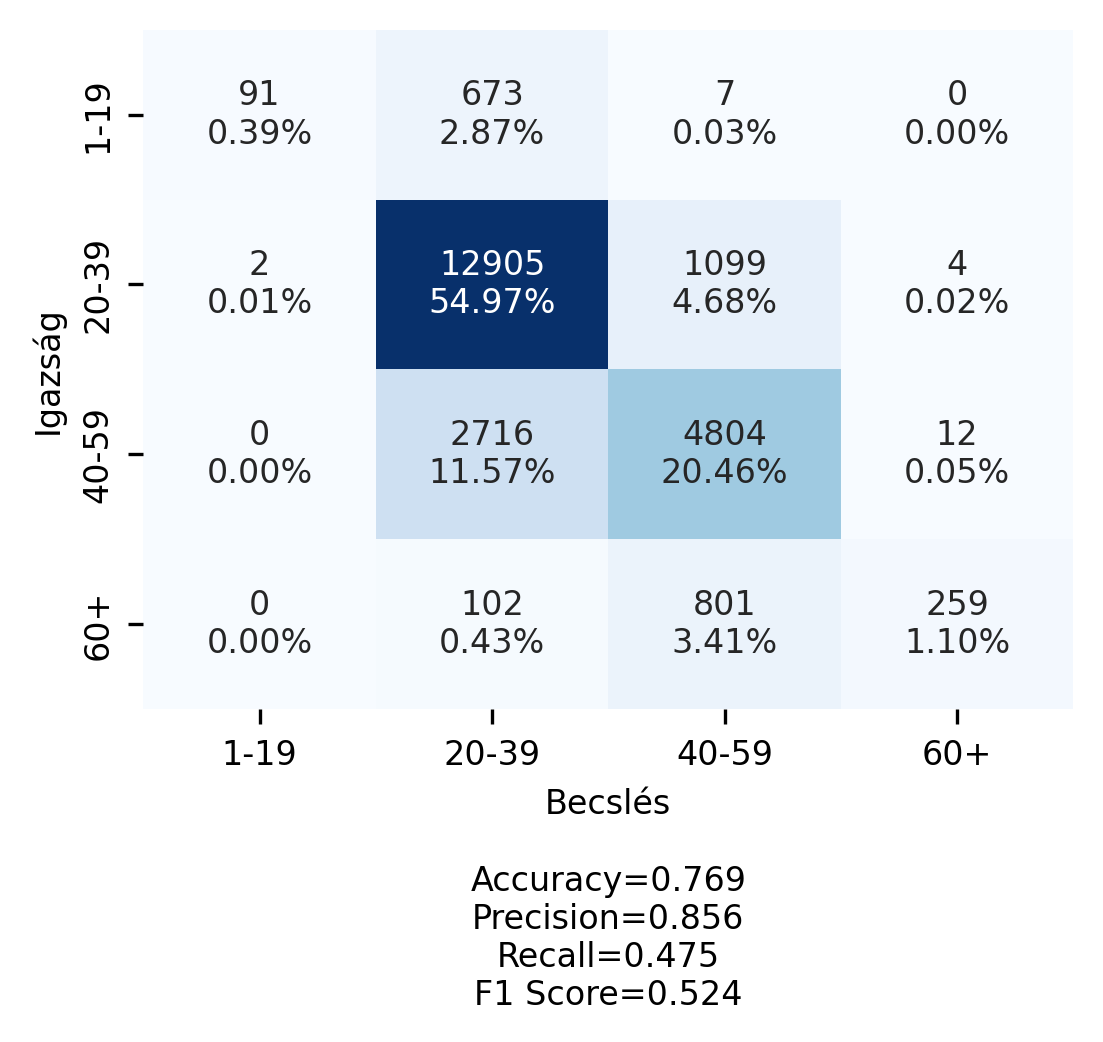
\includegraphics[width=0.7\columnwidth]{figures/conf_age.png}
	\caption{Az életkor osztályozó modell igazságmátrixa és pontossági metrikái.}
	\label{fig:conf_age}
\end{figure}

\subsubsection*{Identifikációs modell}

Az identifikációs modell képes megbecsülni a bemeneti arclenyomat alapján, hogy az melyik személyhez (ID-hoz) tartozik. Erre a feladatra a korábbiaktól eltérően nem gépi tanulási modellt alkalmaztam, hanem távolságmérés alapján határoztam meg a legvalószínűbb személyt. A modellnek szüksége van arclenyomat vektorokra, és hozzájuk tartozó címkékre. Ez alapján az egyes címkékhez tartozó arclenyomatok átlagát számítja ki (amik a centroidok). Új minta becsléséhez a centroidoktól vett távolság alapján találja meg azt az ID-t ami legvalószínűbb találat. A modell működését a \ref{lst:idmodel}. kódrészlet mutatja be.

\begin{lstlisting}[language=python, caption=Az identifikációs modell működése., label=lst:idmodel]
class IDModel:
	def __init__(self, embeddings, ids):
		'''
		embeddings : [np.ndarray] Nx128 - tanito mintak (arclenyomatok)
		ids : [np.ndarray] Nx1 - mintakhoz tartozo azonosito cimkek (pl: 'id00001')
		'''
		self.embeddings = embeddings
		self.ids = ids
		self.unique_ids = np.unique(ids)
		self.centroids = np.zeros((self.unique_ids.shape[0], embeddings.shape[1]))
		for i in range(len(self.unique_ids)):
			id = self.unique_ids[i]
			idx = np.where(ids == id)[0]
			centroid = np.mean(embeddings[idx], axis=0)
			self.centroids[i] = centroid

	def predict(self, new_embeddings):
		# adott arclenyomat es a centroidok tavolsagok osszevetese
		y_hat = np.zeros(len(new_embeddings)).astype('object')
		for i in range(len(new_embeddings)):
			d = np.linalg.norm(new_embeddings[i] - self.centroids, axis=1, ord=2)
			d_min_idx = np.argmin(d)
			y_hat[i] = self.unique_ids[d_min_idx]
		return y_hat

	def score(self, X_test, y_test):
		# becsles pontossaga
		y_hat = self.predict(X_test)
		return np.sum(y_hat == y_test) / len(y_test)
\end{lstlisting}

Összegezve, a három demográfiai adat közül a nemet és a rasszt nagy pontossággal lehet becsülni, míg az életkor becslése nehezebb feladat. Jobb eredmény érhető el akkor, ha kiegyensúlyozottabb életkor arckép adathalmazból indulunk ki. Tekintve, hogy én csak publikusan és ingyenesen elérhető arckép adathalmazokat vizsgáltam, egy valós támadó ennél jobb pontosságot is elérhet, így az eredményem egy alsó becslésnek tekinthető. Az identifikációs modellel is jó pontosságot sikerült elérni, csak néhány esetben adott téves becslést. A négy modell eredményeit a \ref{tab:pontossagok}. táblázat foglalja össze.

\begin{table}[ht]
	\centering
	\begin{tabular}{|c|c|c|c|c|}
		\hline
		& ACC & PREC & REC & F1 \\
		\hline
		\hline
		Nem & 0.988 & 0.987 & 0.989 & 0.988 \\
		\hline
		Rassz & 0.977 & 0.977 & 0.977 & 0.977 \\
		\hline
		Életkor & 0.769 & 0.856 & 0.475 & 0.524 \\
		\hline
		ID & 0.998 & 0.998 & 0.998 & 0.997 \\
		\hline
	\end{tabular}
	\caption{Az osztályozó modellek pontossága}
	\label{tab:pontossagok}
\end{table}
 
%--------------------------------------------------------------------------------------------------
\subsection{Adatvédelmi elemzés} % (1-2 oldal)
\label{sec:adatvedelmi_elemz}

Az előző részben bemutattam, hogy ha a \ref{sec:tamado}. fejezetben definiált támadó jó minőségű arclenyomat adathalmaz birtokában van, akkor az alapján modern gépi tanulási modelleket taníthat be, amelyek képesek további arclenyomatokból személyes adatokat kinyerni. Ebben a részben azzal a kérdéssel foglalkozom, hogy a támadó hogyan tud visszaélni az arclenyomatokból kinyert adatokkal? Egy központi arclenyomat adathalmaz kiszivárgása milyen adatvédelmi kockázatokkal jár?

Kiindulásnak a 29-es munkacsoport anonimizálási eljárásokról szóló véleményét vettem \cite{anon2014}, amelyben szó van az adatvédelmi kockázatok csoportjairól. A csoport véleménye alapján, kockázat elemzés során az alábbi három fő kockázattípust célszerű szem előtt tartani:

\begin{itemize}
	\item Kiválasztásról (singling out): akkor beszélhetünk, ha egy rosszindulatú fél sikeresen be tud azonosítani egy adott személyhez tartozó rekordot az adathalmazon belül.
	\item Összekapcsolhatóság (linkability): legalább két rekord összekapcsolásának képessége, amely ugyanahhoz az érintetthez vagy érintettek csoportjához tartozik. Nem szükséges pontosan beazonosítani az adott személyeket.
	\item Következtetés (inference): ami annak a lehetőségét jelenti, hogy nagy valószínűséggel jelentősen új információ következtethető ki az attribútumok értékeiből.
\end{itemize}

Mivel egy ember arca tipikusan csak kicsit változik idővel, az arcról készült arclenyomat megváltozhatatlan objektumnak tekinthető. Ez azt jelenti, hogy egy személyről készült arclenyomatok különböző alkalmazásokhoz több adatbázisban is szerepelnek nagyon hasonló formában. Ebből adódóan az egyik kockázati lehetőség az, ha a támadó hozzáfér egy privát arclenyomat adathalmazhoz, majd azt egy másik publikusan elérhető adathalmazzal összekapcsolva képes lehet azon személyek újraazonosítására, akik mindkét adathalmazban szerepelnek.

E mellett következtetéses támadás is kockázatot jelent, mivel a támadó az arclenyomat alapján többlet információt képes kikövetkeztetni. Mint azt bemutattam, az arclenyomatok demográfiai adatokat szivárogtathatnak ki. 

A kiválasztás veszélye akkor állhat fent, ha a támadó egy bizonyost személyt próbál beazonosítani, és az arclenyomatokból kinyert extra információk alapján képes leszűkíteni a lehetséges személyek halmazát.

Egy másik adatvédelmi kockázat lehet az arclenyomatok alapján az eredeti arckép rekonstrukciója. A \cite{mai2018reconstruction} szerzői létrehoztak egy szomszédossági dekonvolúciós neurális hálót (NbNet), amely képes visszaállítani az eredeti arcképet egy arclenyomatból. A publikációban bemutatott eredmények alapján, az NbNet magas pontossággal képes visszaállítani az arcképeket, amelyek alapján 2D-s vagy 3D-s arc modell hozható létre. A rekonstruált kép alkalmas lehet arra, hogy arcfelismerő rendszert átverje.

% TODO - ezeket hogyan fogom kivédeni később?

% In [17], a neighborly de-convolutional neural network (NbNet) is designed to reconstruct face images from their deep face features. Experiment results show that NbNet can reconstruct the face images with high accuracy, leading to privacy and security risks.

% Authors in [24] mention two potential threats regarding an attacker’s abilities. One of the hazards is to masquerade the template owner, which means using the biometric template for reconstructing a 2D or 3D model of the template owner’s face and using that model to trick a FR system. 

% The other is the possibility of the attacker to do cross matching between multi- ple databases storing biometric templates, because biometrics are mostly immutable and the same or very similar templates could be stored in multiple databases for different applications. These risks motivate the use of biometric template protection (BTP) schemes that transform biometric templates to make their usage and storage safe, while also keeping their utility.
%----------------------------------------------------------------------------
\section{Az embeddingben kódolt személyes adatok vizsgálata (10-12 oldal)}
\label{sec:5}
%----------------------------------------------------------------------------

\begin{itemize}
	\item elgondolás, ötlet, mire számítottunk
	\item Legfontosabb embedding feature-ök meghatározása (kutatási jelentésből) (4 oldal)
	\item Legfontosabb feature-ök eltávolítása, módosítása milyen hatással van a modell pontosságára (kutatási jelentésből) 
	\item Eredmények kiértékelése (kutatási jelentésből) 
	\item Arclenyomatvektor feature-einek köncsönös összefüggésének vizsgálata (diploma A-ból) (5 oldal)
\end{itemize}

%-----------------------------------------------------------------------------
% Szükségünk volt meghatározni, hogy egy adott modellnek mely koordinátái járulnak leginkább hozzá a modell predikciójához. Feltételezésünk az volt, hogy ha módosítjuk a legfontosabb koordinátákat, akkor azzal jelentősen romlani fognak a modell pontossági metrikái. Egy modell legfontosabb koordinátáit számos módon meg lehet határozni. Ezek közül először a már korábban bemutatott LIME 12 könyvtárat használtuk, ami kifejezetten gépi tanulási modellek értelmezésére szolgál. Annak érdekében, hogy az így kapott eredményeket megerősítsük, több, eltérő módszerrel is megvizsgáltuk a modelleket. A következőkben a rassz osztályozó modell vizsgálatát mutatjuk be.

% 4.1 LIME eredmények
% A LIME könyvtár segítségével meg tudtuk határozni egy adott modell legfontosabb koordinátáit. A következő diagramon az egyes koordináták előfordulási gyakoriságai láthatók. Például az (’f83’, 982) esetén az f83 jelöli az adott koordinátát, az 982 pedig, hogy az 1000 LIME magyarázatból hányszor volt benne a 10 legfontosabb koordináta között.
% % ábra 
% \begin{figure}[ht]
% 	\centering
% 	
\includegraphics[width=0.65\columnwidth]{figures/abra.png}
% 	\caption{abra alatti szoveg}
% \end{figure}

% 4.2 Modell specifikus módszer
% Scikit-learn saját, modell-specifikus implementációját 13 használtuk. Ez a módszer kifejezetten döntési fa alapú modellekre alkalmazható. A döntési fákban magasabban található koordináták nagyobb fontosságúak, mint az alacsonyabban találhatóak. A módszer a Mean Decrease in Impurity és a, Gini importance-en alapul.
% % ábra 
% \begin{figure}[ht]
% 	\centering
% 	
\includegraphics[width=0.65\columnwidth]{figures/abra.png}
% 	\caption{abra alatti szoveg}
% \end{figure}

% 4.3 Permutation importance
% A Permutation importance egy modellfüggetlen módszer. Mi az Eli5 14 könyvtár implementációját használtuk. Egy koordináta fontosságát meghatározhatjuk úgy, hogy megnézzük mennyivel csökken a modell pontossági metrikái (F1, R 2 stb.) ha egy adott koordinátát eltávolítunk. Egy koordináta eltávolítása után újratanítjuk a modellt, és összehasonlítjuk a pontosságát az eredeti modell pontosságával. Mivel újratanítás szükséges, ez egy eléggé számításigényes eljárás.
% % ábra 
% \begin{figure}[ht]
% 	\centering
% 	
\includegraphics[width=0.65\columnwidth]{figures/abra.png}
% 	\caption{abra alatti szoveg}
% \end{figure}

% 4.4 SHAP
% Tree-SHAP 15 használatával elemezhetjük egy-egy megfigyelés esetén a koordináták fontosságát, illetve globális összegző képet is kaphatunk egy adathalmazról. A Tree-SHAP kifejezetten döntési fa alapú modellekre optimalizált módszer, de használható Kernel SHAP is. Rassz predikció esetén halmozott oszlopdiagramon láthatjuk, hogy osztályonként (rasszonként) mely koordináták a legjelentősebbek.  Összegezve őket a LIME-hoz hasonló eredményeket kapunk.
% % ábra 
% \begin{figure}[ht]
% 	\centering
% 	
\includegraphics[width=0.65\columnwidth]{figures/abra.png}
% 	\caption{abra alatti szoveg}
% \end{figure}

% KUTATÁSI JELENTÉS
% -----------------------------------------------------------------------------

% 3 Hálózat effektus vizsgálata 

% Az arclenyomat vektorok korábbi vizsgálata kapcsán beláttuk, hogy a véletlen erdő (angol szakirodalomban random forest) modell döntési fáiban kölcsönös összefüggések állhatnak fent. Az volt a megfigyelésünk, hogy ez a kölcsönös összefüggés hasonlít ahhoz, amit komplex hálózatoknál tapasztalhatóak. Az ilyen hálózatoknál egy csomópont eltávolítása nincs nagy hatással a hálózatra, hanem több csomópont együttes kivételével lehet jelentősen rontani a hálózat összefüggőségén. 

% Először megnéztem, hogy az arclenyomat vektorokon betanított véletlen erdő modellt át lehet-e transzformálni egy gráf reprezentációba. Miután ez sikerült, az volt a hipotézisünk, hogy a rassz predikciós modell és az arc identifikációs modellekből létrehozott gráfok együttes elemzésével találhatunk olyan csomópontokat, amelyek szignifikánsak a rassz predikciós gráfnál, viszont nem szignifikáns az identifikációs modell esetén. Így találhatunk módot az arclenyomat vektorokban hordozott érzékeny információk védelmére. 

% 3.1 Hálózat effektus vizsgálata Iris adathalmazon
% A véletlen erdő modell több döntési fát foglal magában. A vizsgálat során alap esetben 100 fából álló modellt alkalmaztam. Egy adott arclenyomat vektor bemenet esetén az erdőben található összes döntési fa képez egy szavazatot az egyik osztályra. Mivel az arclenyomat vektorokra betanított véletlen erdő rendkívül bonyolult döntési fákból áll, melyek működése ember számára már nem igazán értelmezhető, ezért kezdetben egy jelentősen kisebb adathalmazon: az Iris dataset[ Elérhető: https://archive.ics.uci.edu/ml/datasets/Iris/ ]-en végeztem a döntési fák vizsgálatát. Ez az adathalmaz 4 feature-t (petal width (PW), petal length (PL), sepal width (SW), sepal length (SL) tartalmaz, és 3 kimeneti osztályt, ami 3 féle virágnak felel meg (setosa, versicolor, virginica). 

% \begin{figure}[ht]
% 	\centering
% 	
\includegraphics[width=0.65\columnwidth]{figures/abra.png}
% 	\caption{Az Iris datasetre betanított véletlen erdő egyik döntési fája
% 	vizualizálva.}
% \end{figure}

% Az általam írt algoritmus célja a random forest classifiert átalakítani egy gráf reprezentációba. Az algoritmus először végig halad az erdőben lévő döntési fákon, és egy rekurzív függvény segítségével végig lép a döntési fa egyes csomópontjain. Egy adott csomópont lehet elágazás vagy levél. Elágazás esetén vizsgálni tudjuk az elágazás feltételét, ami egy adott featureből, és egy küszöbértékből (threshold) áll. Az algoritmus működése során feltérképezi a teljes döntési fát, és kigyűjti az egyes levél csomópontokhoz tartozó feltétel rendszereket, azaz milyen feltételeknek kell teljesülnie ahhoz, hogy a döntési fa az adott levélre jusson. Feltételezésem az volt, hogy a fának azon feltételei lesznek szignifikánsak, amelyek gyakran fordulnak elő más feltételekkel együtt.  Definiáltam egy NxN-es mátrixot, ahol N a feature-ök számát jelenti, és a mátrixot 0 értékekkel inicializáltam. A fa feltérképezése során a 2 featurehöz kapcsolódó feltétel együttes megjelenéskor az NxN-es mátrix megfelelő cellájába 1-gyel növeltem az értéket. Ezt a módszert alkalmazva feltérképeztem a véletlen erdő összes döntési fáját, és a fákon belül az összes útvonalat, és feltöltöttem a mátrixot. A 2. ábrán láthatjuk az eredményt. A feature-ök sorra: SL, SW, PL, PW\@. Láthatjuk, hogy leggyakrabban a PW és PL feltételek szerepeltek leggyakrabban (1584 alkalommal) feltöltött NxN-es mátrix (N=4). 

% \begin{figure}[ht]
% 	\centering
% 	
\includegraphics[width=0.65\columnwidth]{figures/abra.png}
% 	\caption{2. Ábra Iris dataset esetén az értékekkel}
% \end{figure}

% Ezt követően létre tudtam hozni egy olyan gráfot, aminek szomszédossági mátrixa a feltöltött NxN-es mátrix. A létrehozott gráf egy teljes gráf, aminek élei súlyozva vannak feltételek együttes megjelenésének számával. 

% \begin{figure}[ht]
% 	\centering
% 	
\includegraphics[width=0.65\columnwidth]{figures/abra.png}
% 	\caption{3. Ábra A szomszédossági mátrix alapján létrehozott gráf. }
% \end{figure}

% 3.2 Hálózat effektus vizsgálata arclenyomat vektorokon 

% Miután megírtam a fent bemutatott algoritmust az Iris datasetre és leteszteltem a működését kisebb, értelmezhető példákon, áttértem az arclenyomat vektorok vizsgálatára. Az általam használt adathalmaz több mint 10 000 arclenyomat vektort tartalmaz, hozzájuk pedig 4 címke tartozik az adott ember rasszára vonatkozóan (fehér, fekete, ázsiai, indiai). Egy arclenyomat vektor 128 feature-t tartalmaz, amelyek valós számok (többnyire (-1, 1) közötti lebegőpontos értékek). Ezen az adathalmazon tanítottam be a rassz predikciós modellt, ami egy Random Forest Classifier 100 döntési fával. A betanított modellen lefuttattam a feltérképező algoritmust, az a korábban leírt módszerek szerint végighalad az összes fa összes útvonalán, és feltöltötte a szomszédossági mátrixot (ami ebben az esetben 128x128-as méretű).  A szomszédossági mátrix alapján már létrehozható egy teljes, súlyozott gráf.

% Feltételezésem az volt, hogy a gráf struktúrájából adódóan meg tudok határozni a modell számára szignifikáns feature-öket amelyeket, ha eltávolítunk az adathalmazból, a modell pontossága jelentősen romlani fog. Egy feature fontosságát úgy határoztam meg, hogy a súlyozott gráf feature-höz tartozó csomópontjának vettem a fokszámát (csomóponthoz tartozó élek súlyainak összegét).  A fokszámokat ki tudtam számolni a szomszédossági mátrix alapján. A kapott eredményeket csökkenő sorrendbe rendeztem, és összehasonlítottam a Sci-kit learn feature\_importance[ Scikit-learn feature importance függvénye: link] módszerével kapott eredménnyel. A két módszerrel nagyon hasonló eredményt kaptam, amit láthatunk a 4. ábrán. 

% \begin{figure}[ht]
% 	\centering
% 	
\includegraphics[width=0.65\columnwidth]{figures/abra.png}
% 	\caption{A RFC legfontosabb feature-ei csökkenő sorrendben.  Bal oldalon az általam írt algoritmus eredménye, jobb oldalon a sci-kit learn feature\_imporance függvényével kapott eredmény.}
% \end{figure}

% \begin{figure}[ht]
% 	\centering
% 	
\includegraphics[width=0.65\columnwidth]{figures/abra.png}
% 	\caption{5. Ábra A modell pontosságának kirajzolása az eltávolított feature-ök számától függően.}
% \end{figure}

% Miután a modell számára legfontosabb feature-öket meghatároztam, megnéztem hogyan változik a RFC pontossága, ha eltávolítom a legfontosabb feature-öket. Mit láthatjuk az 5. ábrán, a modell pontossága nem romlik jelentően még akkor sem, ha feature-ök több mint felét eltávolítottuk.
%----------------------------------------------------------------------------
\section{Javaslat a kockázatok kiszűrésére}
\label{sec:6}
%----------------------------------------------------------------------------

% TODO
% rövid szöveg ide

\subsection{Adversarial módszerek}

A korábban vizsgált megközelítéssel sajnos nem sikerült jó eredményeket elérni. A modell robusztusságából adódóan néhány jellemző kivételével nem romlik a modell pontossága, és a hálózat effektus feltételezés sem bizonyult helyesnek. Következő próbálkozás az adversarial attack módszerek irányába indult. Adversarial examplenek nevezzük azt a mintát, amelyet, ha kis mértékben módosítunk képes becsapni egy adott machine learning modellt. Ezt a gyakorlatban egy kis mértékű pontosan kiszámított zaj hozzáadását jelenti, miközben a modell hibáját maximalizálja. 

Annak érdekében, hogy belássuk, működhetnek az ilyen módszerek azt tűztem ki célul, hogy mutassam be néhány félig manuálisan készített példán keresztül, hogy az arclenyomatok kis mértékű módosításával be lehet csapni a random forest classifier modellünket. Ehhez készítettem egy újabb algoritmust, amelyet előbb Iris dataseten teszteltem a könnyebb értelmezhetőség érdekében, majd miután működött áttértem az arclenyomat vektorok használatára.

Az algoritmus mögöttes ötlete abból ered, hogy ha megvizsgáljuk az egyes döntési fákat, találhatunk olyan elágazásokat (feltételeket) ahol egy adott arclenyomat vektor jellemzőinek értéke a döntési küszöbértékhez meglehetősen közeli értéket vesz fel. Az ilyen esetekben ezeknek a jellemzőknek kis módosításával el lehet érni azt, hogy a döntési fa feltétele átbillenjen, és másik útvonalon halad a következő elágazásig. Ez a módosítás önmagában még nem garantálja azt, hogy a döntési fa kimenete megváltozik, mivel előfordulhat, hogy a kitérítés után egy másik levélre jut, ami ugyanazt az eredményt adja, mint az eredeti kimenet. Ezt szemlélteti a következő példa.

\begin{figure}[ht]
	\centering
	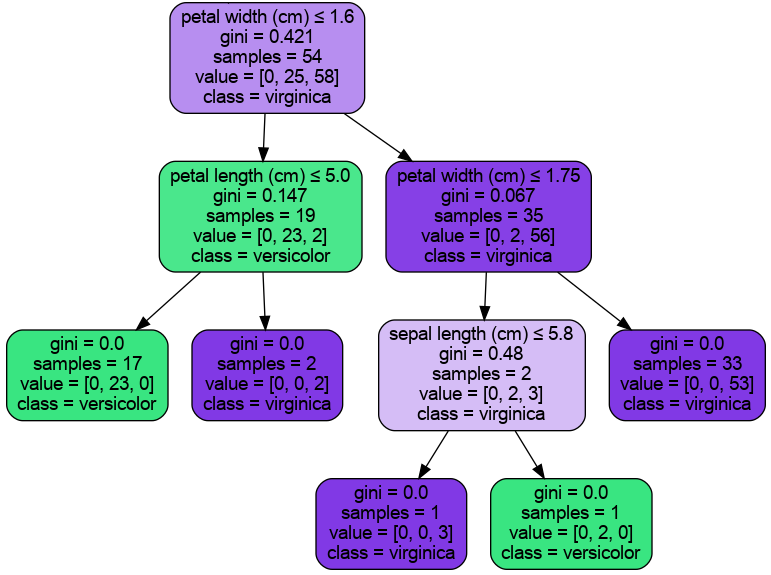
\includegraphics[width=0.9\columnwidth]{figures/adverse_tree_graph.png}
	\caption{Döntési fa részlete, ami az Iris datasetre lett betanítva.}
	\label{fig:iris_tree}
\end{figure}

Tegyük fel, hogy az általunk vizsgált mintában a petal width jellemző értéke 1,55 cm, petal length értéke 4,5 cm. Ezt a mintát a \ref{fig:iris_tree}. ábrán látható döntési fa alap esetben ``versicolor'' kategóriába sorolná. A döntési fa a legfelső elágazásnál petal width $\le$ 1.6 cm feltétel szerepel. Belátható, hogy a bemeneti érték kis módosításával (1.55 + 0.05) átbillenthető a feltétel teljesülése, és az eredeti bal ág helyett jobb ág irányába halad tovább a döntéshozatal, ezzel potenciálisan téves predikcióra vezethető a fa. Azt is láthatjuk ebben a példában, hogy ha a mintánkban a sepal length jellemző értéke nagyobb mint 5,8 cm, akkor újból ``versicolor'' levélre jutunk, tehát előfordulhat, hogy hiába tévesztettük meg a döntési fát egy ponton, a fa predikciója továbbra is változatlan marad.

A véletlen erdő sok döntési fát tartalmaz, amelyek mind képeznek egy-egy szavazatot az egyik kimenetre, ezért egyetlen fa becsapása legtöbb esetben nem elegendő a teljes véletlen erdő kimenetének módosítására, így a bemeneti arclenyomat vektor olyan módosítása szükséges, ami egyidejűleg több döntési fa predikcióját is képes eltéríteni.

\subsubsection*{Adversarial módszer fejlesztése Iris adathalmazon}

Az Iris dataseten betanított random forest classifieren a korábbihoz hasonlóan egy rekurzív függvényt használtam, ami végighalad az erdőben található egyes döntési fákon, és az elágazásoknál vizsgálja az adott feltételhez tartozó jellemző bemeneti értékét, és küszöbértékét. Az algoritmus első verziója egy adott bemenetre keresi azokat a küszöbértékeket, amelyek a bemenettől maximum 10\%-kal térnek el. Ezeknél a feltételeknél van lehetőségünk kis módosítással megtéveszteni a fát. Az ilyen eseteknél a program kiírja melyik fáknál, és melyik jellemző értéknél van megfelelően kis eltérés a küszöbértékhez képest.

\begin{lstlisting}[caption={A döntési azon elágazási pontjai, amelyek kis jellezőmódosítással átbillenthetőek.}]
Tree: 0 out: 1  feature: PL  4.9 <= 4.85, diff: -0.05
Tree: 1 out: 1  feature: PL  4.9 <= 4.95, diff: 0.05
Tree: 2 out: 1  feature: PW  1.5 <= 1.55, diff: 0.05
Tree: 2 out: 1  feature: PL  4.9 <=  5.0, diff:  0.1
Tree: 3 out: 1  feature: PL  4.9 <= 4.95, diff: 0.05
Tree: 4 out: 1  feature: PL  4.9 <= 4.95, diff: 0.05
Tree: 5 out: 1  feature: PL  4.9 <= 4.95, diff: 0.05
(*@\raisebox{-1pt}[0pt][0pt]{$\quad\vdots$}@*)
Tree: 99 out: 1  feature: PW  1.5 <= 1.55, diff: 0.05
\end{lstlisting}

Az eredményeket megpróbáltam valamilyen módon összesíteni, de voltak esetek mikor a küszöb érték alatt volt a jellemző értéke kicsivel, volt mikor fölötte. Az könnyen látható volt, hogy a petal length feltétel szerepelt a 100 fából leggyakrabban, így annak a módosításával próbálkoztam.

A módszer szemléltetésére kerestem egy mintát, ahol a véletlen erdő fái egyértelműen döntöttek az egyik osztály mellett, és a bemenet kis módosításával próbáltam elérni, hogy minél több fa téves predikcióra jusson. Az alábbi mintánál eredetileg a 96 szavazott a ``versicolor'' osztályra, majd egyetlen jellemző viszonylag kis módosítással (petal width 4,9-ről 5.05-re lett növelve) sikerült elérni, hogy a fák többsége ``virginica'' osztályra szavazzon.

\begin{lstlisting}[caption={A véletlen erdő kimenetének manipulációja.}]
Eredeti értékek:
[6.9 3.1 4.9 1.5]
Módosított értékek:
[6.9  3.1  5.05 1.5 ]
Módosítás mértéke:
0.88%

Fa szavazatok:
módosítás előtt [ 0. 96.  4.]
módosítás után  [ 0. 40. 60.]
\end{lstlisting}

\subsubsection*{Adversarial módszer arclenyomat vektorokon}

Az Iris datasetes példán elért eredmények után az algoritmus fejlesztését az arclenyomat vektorokról készült adathalmazon folytattam. Az algoritmus működése során továbbra is végighalad a döntési fán és a bemenet értékeitől függően lép egyik elágazásról a következőre. Ennél a verziónál is detektáltam az olyan elágazásokat, ahol a bemeneti érték egy előre definiált tartományon belül tér el a küszöbértéktől. Minden alkalommal, mikor detektál az algoritmus egy ilyen elágazást, az elágazás mindkét ágán folytatja a fa feltérképezését egészen addig, amíg levél csomóponthoz nem jut. A levélhez eljutva megnézi, hogy az adott levélhez tartozó kimeneti osztály megegyezik-e a mintához tartozó címkével, vagy sem.

Itt az az elgondolás, hogy minden esetben mikor könnyen átbillenthető csomóponthoz jutunk, eldönthetjük, hogy melyik úton érdemes tovább haladni. Az egyes lehetséges utakat feltérképezve ki tudjuk választani azt az utat, ami téves predikcióhoz vezet, illetve, ha több ilyen út van akkor ki tudjuk választani azt, amelyikhez a legkisebb beavatkozás szükséges. 

Az algoritmus végig megy a véletlen erdő összes döntési fáin, kivéve azokat, amelyek alapból is téves predikciót adnak, mivel ezeken nem kell módosítanunk.

\begin{lstlisting}[caption={Algoritmus futtatása egy adott arclenyomat vektorra.}, label=lst:tree_diffs]
Tree: 4, output: 3
		f10  diff: -0.0267
Tree: 4, output: 2
		f88  diff: -0.04035
Tree: 9, output: 3
		f77  diff: -0.02279
Tree: 11, output: 3
		f93  diff: 0.002902
		f57  diff: -0.008323
		f82  diff: -0.007353
Tree: 11, output: 3
		f93  diff: 0.002902
		f57  diff: -0.008323
		f91  diff: 0.02286
(*@\raisebox{-1pt}[0pt][0pt]{$\quad\vdots$}@*)
Tree: 48, output: 1
		f93  diff: 0.002753
\end{lstlisting}

Az algoritmus lefuttatható egy adott arclenyomat vektorra. Lefuttatás során a \ref{lst:tree_diffs}. kódrészlethez hasonló információt kapunk. Eredményül egy listát kapunk, ami felsorolja azokat a fákat a random forest classifier-en belül, amelyek kis (10\% alatti) input módosítással megtéveszthetőek. Fel van tüntetve a fa sorszáma, illetve a fa megtévesztés utáni predikciója (ennél a példánál helyes predikció 0 lenne.) Egy fához fel vannak sorolva azok a jellemzők amelyeket módosítani kell a fals predikció eléréséhez, ahol a ‘diff’ érték mutatja a szükséges módosítás mértékét. Ha több jellemző van felsorolva, például Tree 11-nél akkor azok a módosítások ÉS kapcsolatban állnak egymással.

Megfigyelhetjük ezen a példán, hogy egy fához több téves predikció is tartozhat, attól függően, hogy melyik jellemzők értékét változtatjuk. Például a Tree 4 esetén elérhetünk 3-mas vagy 2-es predikciót is. Az is előfordulhat, hogy egy döntési fán belül több útvonal vezet egy téves predikcióhoz, például Tree 11 esetén három féle képen kaphatunk 3-mas predikciót. Ilyenkor a kisebb módosítást igénylő út a preferált. 

Jelenleg az algoritmus félig automatikus működésű. A lefuttatás során nem fog módosítani az eredeti mintán, azt manuálisan kell elvégezni. Ez az egyik terület, ahol tovább szeretném fejleszteni ezt a megoldást, hogy képes legyen kiszámolni az optimális átalakítást, ahol a legkisebb zaj hozzáadásával megtéveszthető a véletlen erdő becslése. Jelenleg kézzel lehet összeválogatni az egyes jellemzők módosításait, és az alapján összerakni egy zaj vektort. A feladat nehézségét az adja, hogy lehetnek ellentmondásos feltételek (egyik fa növelni szeretné a jellemző értékét, másik pedig csökkenteni), illetve az is előfordulhat, hogy egy jellemző módosítás hatására az egyik fánál korábbi rossz predikció átvált helyesre. Az jellemző módosítások optimális kombinációjának megtalálása nem egyszerű feladat.

\begin{lstlisting}[language=python, caption={Korábbi elemzés alapján manuálisan elvégzett jellemző módosítások.}, label=lst:tree]
# feature modositasok
x_ = x.copy()

x_[:,10] += -0.0268  # Tree 4, Tree 17
x_[:,77] += -0.0228  # Tree 9
x_[:,43] += -0.02737  # Tree 13, 29, 31
x_[:,8] += 0.02539  # Tree 24
x_[:,88] += -0.0314  # Tree 35
x_[:,105] += -0.02175  # Tree 37
x_[:,44] += 0.02302  # Tree 41

print('tree votes:')
print(count_votes(x))
print(count_votes(x_))

# kimenet:
'''
tree votes:
[30. 4. 3. 13.]
[20. 4. 4. 22.]
'''
\end{lstlisting}

A \ref{lst:tree}. kódrészleten láthatjuk, hogyan végezhető el a korábban megállapított jellemzők módosítása. Az eredeti arclenyomat vektor értékeit az ‘x’ változó tárolja. A random forest classifier 50 fából áll, melyek közül 30 fa eredetileg 0 predikciót képez. Egy-egy jellemző módosításnál kommentben megneveztem azokat a fákat, amelyeknek a módosítás hatására átváltanak a helyes (0) predikcióról egy másik értékre. Összesen 10 fa megtévesztésével elérhettük azt, hogy a teljes erdő téves predikciót produkál a módosított mintára. 

Fontos még megjegyezni, hogy összességében elég kis módosítással sikerült elérni ezt az eredményt. Az arclenyomat vektor 128 jellemző közül elegendő volt 7-et kiválasztani, és azokat is maximum 10\%-ban módosítani. A feltételezésem az, hogy ez a módosítás elegendően specifikus és kis méretű, hogy ezzel még megőrizhető egy arclenyomat vektorok alapján betanított identifikációs modell pontossága, de ezt még nem teszteltem le.

\subsubsection*{Összefoglalás}

Ebben a dokumentumban összefoglaltam a félév alatt Diplomatervezés 1 tantárgy alatt elvégzett munkám eredményeit. A félév első felét hálózat effektus hipotézis vizsgálatával töltöttem, ami végül nem vezetett eredményre. Bemutattam a hipotézis mögött rejtő gondolatmenetet és a kísérleteket.

Később az adversarial attack jellegű algoritmus fejlesztésével foglalkoztam. Bemutattam a döntési fák vizsgálatának módszerét és implementálását. Részleteztem az algoritmus fejlesztésének menetét, az egyszerűbb feladatok megoldását, majd az arclenyomat vektorokon elért eredményeket.Jelenleg az algoritmus félig automatikus működésű, azaz a döntési fák elemzése után kézzel kell összeállítani az arclenyomat vektorok módosítását. Az egyik főbb továbbfejlesztési irány az lenne, hogy az algoritmus képes legyen közel optimális zaj generálására, amellyel a véletlen erdő predikciója becsapható. 

E mellett meg kell még vizsgálnom, hogy az arclenyomat vektor módosítása során mennyire romlik az arclenyomat felhasználhatósága egyéb célokra, például identifikációra? Sikerül-e reprodukálni az eredményeket más adathalmazokon betanított modelleken? További irány lehet más területeken sikeresen alkalmazott adversarial attack módszerek kipróbálása véletlen erdő modellre, és az eredmények összevetése.

\subsection{Kriptográfiai módszerek}

% 4-5 oldal
% \begin{itemize}
% 	\item cancelable biometrics
% 	\item motiváció, titkosítási módszerek előnyei (0.5 - 1 oldal)
% 	\item klasszikus hashelés, LSH, random projekció (1 - 1,5 oldal)
% 	\item klasszikus titkosítási, homomorfikus, hogy képzelhető el arcfelismerésnél  (1-1,5 oldal)
% \end{itemize}

A korábban bemutatott módszerek célja az volt, hogy a [REF]. fejezetben bemutatott támadót feltételezve, egy arcfelismeréshez használt központi arclenyomat adathalmaz feltörése esetén az arclenyomatokból ne lehessen érzékeny adatokat kinyerni. Ennek érdekében olyan módszereket vizsgáltam, amelyek az arclenyomatok kis módosításával meggátolná a személyes adatok szivárgását. Ebben a fejezetben egy másik megközelítést, olyan titkosítási módszereker mutatok be, amelyek alkalmazhatóak az arcfelismerés területén.

Egy arclenyomat adathalmaz feltörése azért kritikus biztonsági szempontból, mert az ember arcáról készült arclenyomatok nem változnak idővel. Míg felhasználói jelszavak kiszivárgása esetén van lehetőség a jelszó módosítására, arcfelismerő rendszerek esetén nincs lehetőség arra, hogy valaki megváltoztassa az arclenyomatát. E mellett kockázatot jelen az is, hogy ugyanaz a biometrikus azonosítót több hitelesítési rendszerben is használhatnak. Ha az egyik alkalmazás kiszivárogtatja a biometrikus azonosítót, az összes többi rendszert veszélyezteti, ami ugyanazt a biometrikus adatot használja.

A titkosítási módszerek lényege az, hogy az arclenyomatokat nem eredeti formájukban tároljuk, hanem titkosított formában. A biometrikus adatokat valamilyen módszerrel áttranszformálják, majd transzformált állapotban tárolják. A transzformáció lehet invertálható, vagy nem invertálható (azaz végleges). A titkosítás módjára léteznek biometrikus sablonvédelmi módszerek \cite{patel2015cancelable}, amelyeket biometrikus adatok (pl. újlenyomat, arclenyomat) tárolására fejlesztettek ki. Ezeket mutatom be részletesebben a továbbiakban.

% visszaalakítás összehasonlításhoz

% kiszivárgás nem jelent problémát mert újat lehet generálni

\subsubsection{Hashelési módszerek}

% ezt ki lehet egészíteni azzal, hogy különböző cégek különböző hash fv-t használhatnak
Az arclenyomatok titkosításához egy egyszerű és bevállt módszer lenne a szabványos titkosítási technikák, mint például a hash függvények alkalmazása. A hash függvények a biometrikus adatok védelmére lehet használni, mivel hesselés során az adat végleges átalakításon megy keresztül. A hash függvényeket szinte lehetetlen invertálni, így ha a hesselt arclenyomatok kiszivárognak, azokból az eredeti arclenyomatokat nem lehet visszanyerni. E mellet előnye még a módszernek az, hogy különböző applikációk eltérő hash függvényt használnának, így ha az egyik applikáció adatbázisát feltörik, az nem jelent veszélyt a többi applikációra.

Egy probléma van a klasszikus hesselési eljárásokkal, hogy a hash függvény kimenete már kicsiben eltérő bemenetre is teljesen eltérő lesz. Ez azért probléma, mert a legtöbb biometrikus adat esetén, beleértve az arclenyomatokat is, a környezeti hatások befolyásolhatják az arclenyomatok pontos értékeit. Például egy személyről eltérő fényviszonyokban, vagy más szögekből készült arcképekből származtatott arclenyomatok kis mértékben eltérnek egymástól. Az egymáshoz közeli arclenyomatok hesselés során nagyban különbölő kimenetet kapnak, és emiatt nem alkalmasak összehasonlításra \cite{patel2015cancelable}. 

Ez a probléma megoldható, ha egy olyan hash függvényt használunk, ami a közeli pontoknak azonos kimenetet képez. Az ilyen módszereket lokalitás érzékeny hash függvényeknek hívjuk (angol szakirodalomban locality sensitive hashing, röviden LSH) amelyeket használnak például képek hasonlóságának mérésére \cite{jing2008visualrank}. A lokalitás érzékeny hash függvények létezését a Johnson-Lindenstrauss lemma mondja ki, mi szerint több magas dimenziójú térbeli pont leképezhető alacsonyabb dimenziójú térbe oly módon, hogy bármely két pont közötti távolság közel azonos marad  \cite{johnson1984extensions}. Az LSH függvények segítségével adatpontok csoportosíthatóak, hiszen a hasonló bemeneteket nagy valószínűséggel azonos csoportba sorolja az algoritmus. A \ref{fig:lsh}. ábrán látható a különbség a klasszikus hashelés és az LSH között.

\begin{figure}[ht]
	\centering
	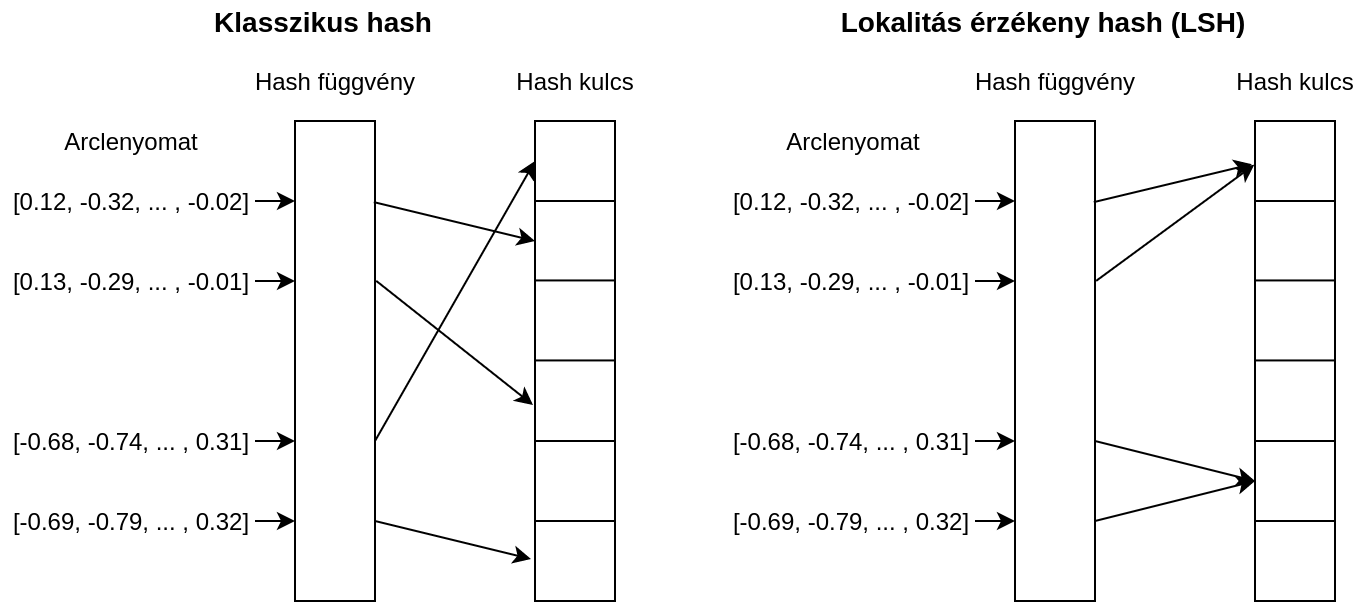
\includegraphics[width=1\columnwidth]{figures/lsh.png}
	\caption{Bal oldalon a klasszikus hesselés látható, jobb oldalon az LSH.}
	\label{fig:lsh}
\end{figure}

Az LSH módszerek már alkalmasak lehetnek arcfelismerő rendszerek esetén az arclenyomatok biztonságos tárolására. Az arcfelismerő rendszer tárolja a hash függvényt, illetve a személyek arclenyomatait hesselt formában. Hitelesítés során az ismeretlen személy arcképéből az arcfelismerő rendszer arclenyomatot képez, amelyet a rendszerben tárolt LSH függvénnyel hesselik, majd összevetik a tárolt hessekkel. Ha a bemeneti képből képzett hash megfelelően közel van az egyik eltárolt sablonhoz, akkor sikeres a hitelesítés.


% A simple approach would be to use standard encryption techniques such as hash func- tions or encryption to enhance the privacy. Hash functions have been used to protect biometric templates in which one-way func- tions are used to compute a digest. Even though these functions are almost impossible to invert, they produce a significantly differ- ent digest even with minor changes in the input. In practice, all biometric templates change with environmental conditions. For instance, face and iris biometrics are significantly affected by illu- mination variations. Therefore, these functions cannot be used directly in practice despite being theoretically very strong as they apply only to exact data.

\subsubsection{Titkosítási módszerek} % kripto kulcs alapú

% klasszikus titkosítási módszer hogy működik
% probléma: összehasonlításhoz vissza kell állítani
% erre megoldás a homomorfikus titkosítás

% titkosító algoritmus és kulcs segítségével titkosított adat -> csak az tudja olvasni aki rendelkezik az olvasáshoz szükséges kulccsal

% when data are encrypted, they need to be decrypted to carry out matching. This creates a possible attack point to get access to the decrypted templates. 

A titkosítás vagy rejtjelezés olyan kriptográfiai eljárás, amellyel valamilyen adatot egy titkosító algoritmus kulcs segítségével átalakítja olyan formára, amely ember számára olvashatatlan. Az adat olvasását csak az teheti meg, aki rendelkezik az olvasáshoz szükséges kulccsal. A titkosított adatot gyakorlatban szinte feltörhetetlenek. Ennek ellenére arclenyomatok védelmére mégsem ideális a klasszikus titkosítási módszerek. 

Ennek oka az, hogy az arcfelismerő rendszer működéséhez szükséges az azonosítandó személy arclenyomatát a rendszerben tárolt arclenyomatokkal összevetni valamilyen módszerrel, például az arclenyomatok közötti euklideszi távolság alapján. Ha az adatbázisban tárolt arclenyomatok titkosítva vannak, akkor azokat elősször szükséges dekódolni az összehasonlításhoz, mert a titkosított adatokon közvetlenül nem tudjuk elvégezni a szükséges műveleteket. 

A titkosított adatokkal általánosságban az a probléma, hogy ahhoz, hogy műveleteket végezzünk rajtuk dekódolni kell. Dekódolássval viszont egy lehetséges támadási pont nyílik meg a rendszerben, ahol lehetséges hozzáférni az eredeti adatokhoz.

Van erre a problémára egy hatékony megoldás amit homomorfikus titkosításnak hívnak. A homomorfikus titkosítás egy publikus kulcsot használ az adat titkosítására. A klasszikus titkosítási módszerektől eltérően a homomorfikus titkosítással lehetséges a titkosított adatokon matematikai műveleteket végezni. A titkosított adatokon végzett műveletek eredménye is titkosított adat lesz, amelyet dekódolva ugyanazt az eredményt kapjuk, amit a titkosítatlan adatokon elvégzett ugyanezen műveletek eredményeztek volna. Így a hitelesítési fázisban nics szükség a titkosított adatokat dekódolni, azonok közvetlenül el lehet végezni az összehasonlítást. 

A homomorfikus titkosításnak három fő típusa van:
% TODO ezt fact checkelni mert lehet nem igaz amit írok
\begin{itemize}
	\item \textbf{Partially homomorphic encryption}: Ebben az esetben csak bizonyos matematikai műveleteket lehet végrehajtani a titkosított adatokon.
	\item \textbf{Somewhat homomorphic encryption}: Korlátozott számú műveletet támogat, amelyek csak meghatározott számú alkalommal hajthatóak végre.
	\item \textbf{Fully homomorphic encryption}: A teljesen homomorfikus titkosítás (FHE) minden műveletet támogat, és a műveletek korlátlan számmal hajthatóak végre. Ez a legerősebb típusa a homomorfikus titkosításnak. 
\end{itemize}

A homomorfikus titkosításnak jelenleg az a legnagyobb hátránya, hogy magas a számításigénye az eljárásnak, ezért elég lassú, és e miatt nem praktikus még az alkalmazása. Az arcfelismerő rendszereknél alkalmazható lehet egy olyan részlegesen homomorfikus titkosítást alkalmazni, ami gyorsabb működésű mint az FHE támogatja az összeadást, így távolságméréshez euklideszi távolság helyett lehet például Manhattam távolságot használni.

% A homomorf titkosítás széles körű elterjedésének legnagyobb akadálya az, hogy még mindig nagyon lassú – olyan lassú, hogy még nem praktikus sok alkalmazáshoz. azonban

% Just like other forms of encryption, homomorphic encryption uses a public key to encrypt the data. Unlike other forms of encryption, it uses an algebraic system to allow functions to be performed on the data while it’s still encrypted. Then, only the individual with the matching private key can access the unencrypted data after the functions and manipulation are complete. This allows the data to be and remain secure and private even when someone is using it. 

% There are three main types of homomorphic encryption: partially homomorphic encryption (keeps sensitive data secure by only allowing select mathematical functions to be performed on encrypted data); somewhat homomorphic encryption (supports limited operations that can be performed only a set number of times); fully homomorphic encryption (this is the gold standard of homomorphic encryption that keeps information secure and accessible).

% The biggest barrier to widescale adoption of homomorphic encryption is that it is still very slow—so slow it’s not yet practical to use for many applications. However

% A homomorf titkosításnak három fő típusa van: részlegesen homomorf titkosítás (biztonságban tartja az érzékeny adatokat azáltal, hogy titkosított adatokon csak bizonyos matematikai függvények végrehajtását engedélyezi); kissé homomorf titkosítás (korlátozott műveleteket támogat, amelyek csak meghatározott számú alkalommal hajthatók végre); teljesen homomorf titkosítás (ez a homomorf titkosítás aranystandardja, amely biztonságosan és hozzáférhetően tartja az információkat). 
% A homomorf titkosítás széles körű elterjedésének legnagyobb akadálya az, hogy még mindig nagyon lassú – olyan lassú, hogy még nem praktikus sok alkalmazáshoz. azonban

% % %----------------------------------------------------------------------------
% \section{Bevezetés (2-3 oldal)}
% %----------------------------------------------------------------------------

% Advances in machine learning ...

% Felépítés:
% \begin{itemize}
% 	\item gépi tanulás advancements
% 	\item gépi tanulás jelentősége \\ napjainkban egyre elterjedtebb, hol használják
% 	\item deep learning elterjedése, használata
% 	\item adatgeneráló eljárások \\ motiváció, fajták, felhasználás
% 	\item embeddingek, face embedding
% 	\item arcfelismerés bemutat: egyre gyakrabban használnak kamerát \\ térfigyelő kamerák, ...
% 	\item valami szemléltető ábra hasznos lenne, működés magyarázatához. ábra: emberek -> kamera -> képet készít -> embedding -> tárolás, feldolgozás
% 	\item adatvédelmi kockázat
% 	\begin{itemize}
% 		\item pl kína szociális kreditrendszer
% 		\item  arcfelismerő rendszerek tökéletlenségét kihasználó hozzáférési támadások (pl. "face morphing", "presentation attacks", stb.)
% 		\item a gépi tanulás hibáiból bekövetkező diszkriminációk és pontatlanságok
% 		\item az arclenyomatokból gépi tanulási eljárásokkal kiszedhető személyes információk kiszivárgása
% 	\end{itemize}
% 	\item motiváció, mit vizsgálok a dolgozatban
% 	\item diplomaterv felépítése
% \end{itemize}

% %----------------------------------------------------------------------------
% \section{Irodalomkutatás (15-20 oldal)}
% %----------------------------------------------------------------------------
% Átfogó jelleggel mutassa be az adat generáló gépi tanulási megoldásokat!

% Az egészet időrendi sorrendben kéne felvezetni -> régi: Boltzman -> új \\
% Fontos része: mögöttes ötlet -> embedding / látens térbeli reprezentáció

% Syamese network -> ez is embeddingeket hoz létre.

% Probléma felvetés:
% Ötlet: általánosítható legyen a módszer akár többféle alkalmazásban is. -> Deep fake reprezentáció is tartalmazhat személyes adatot

% Felépítés: \\
% Adatgeneráló eljárások (4-5 topic ~3-4 oldal)
% \begin{itemize}
% 	\item felvezető ~ 4 oldal 
% 	\begin{itemize}
% 		\item supervised / unsupervised learning (mygreatlearning GAN)
% 		\item discriminate / generative models
% 		\item density estimation (mygreatlearning Boltz)
% 		\item generative modellek csoportosítása (Explicit, implicit) (mygreatlearning Boltz)
% 	\end{itemize}
% 	\item boltzman machines (~3)
% 	\begin{itemize}
% 		\item extract latent space from data
% 		\item Markov chain
% 		\item graphical models -> remove mb
% 		\item Markov property
% 		\item BM and RBM structure - how it works
% 		\item Usage today (spoiler alert: not much)
% 		\item ha kell több emlélet: deeplearningbook.org
% 	\end{itemize}
% 	\item Generative adversarial network (GAN) (~3-4)
% 	\begin{itemize}
% 		\item mygreatlearning explanation
% 		\item input noise generates the new data
% 		\item Generator and Discriminator
% 		\item they compete and get better -> discriminator cant tell anymore
% 		\item GAN példák -> TODO
% 	\end{itemize}
% 	\item variational auto-encoder (~2-3)
% 	\begin{itemize}
% 		\item mygreatlearning explanation
% 		\item auto encoder úgy általában. (dim(input) = dim(output))
% 		\item compress to small representation -> uncompress
% 		\item encoder, 'code', decoder
% 		\item variational auto encoder mitől "variational"
% 		\item data follows normal distribution -> mean, std
% 		\item how it's trained (reparameterization trick, loss function)
% 		\item példa alkalmazásra: deep fake -> TODO
% 	\end{itemize}

% 	\item deep metric learning -> embedding (~1-2)
% 	\begin{itemize}
% 		\item 
% 	\end{itemize}
% 	\item syamese networks (~2 oldal)
% 	\begin{itemize}
% 		\item 
% 	\end{itemize}
% 	\item triplet loss
% 	\begin{itemize}
% 		\item 
% 	\end{itemize}
% \end{itemize}

%----------------------------------------------------------------------------
% \section{Probléma bemutatása (4-6 oldal)} 
% %----------------------------------------------------------------------------
% \begin{itemize}
% 	\item arcfelismerő rendszerek működése
% 	\item arcfelismerés problémakör
% 	\item arclenyomat vektor
% \end{itemize}

%----------------------------------------------------------------------------
\section{Arclenyomatok adatvédelmi elemzése (8-10) oldal}
%----------------------------------------------------------------------------
\begin{itemize}
	\item módszertan, támadómodell -> hozzáfér datasethez
	\item adatgyűjtés -> vgg és imdb datasetek előállítása (2-4 oldal)
	\item random forestek betanítása -> race, sex, age, +1 valami?
	\item betanítás utáni eredmények -> accuracy, ROC curve
	\item adatvédelmi elemzés -> milyen riskek vannak (munkacsoport szerint)
	\item pl: több info kiderülése 1 emberről probléma, adatszivárgás: le tudja szűkíteni, hogy ki lehet az, singling out, vagy lehet arcot rekonstruálni az embeddingből, újraazonosítás.
\end{itemize}

%----------------------------------------------------------------------------
\section{Az embeddingben kódolt személyes adatok vizsgálata (10-12 oldal)}
%----------------------------------------------------------------------------
\begin{itemize}
	\item Legfontosabb embedding feature-ök meghatározása (kutatási jelentésből)
	\item Legfontosabb feature-ök eltávolítása, módosítása milyen hatással van a modell pontosságára (kutatási jelentésből) 
	\item Eredmények kiértékelése (kutatási jelentésből) 
	\item Arclenyomatvektor feature-einek köncsönös összefüggésének vizsgálata (diploma A-ból)
\end{itemize}


%----------------------------------------------------------------------------
\section{Javaslat a kockázatok kiszűrésére (10+ oldal)}
%----------------------------------------------------------------------------
\begin{itemize}
	\item Döntési fák félrevezetése embeddingek kis módosításával (diploma A-ból)
	\item Adversarial attack módszerek körbejárása
	\item javaslat: titkosítás, lsh, random projekció (source: MNB arcfelismerés)
\end{itemize}

%----------------------------------------------------------------------------
\section{Összefoglalás (1-3 oldal)}
%----------------------------------------------------------------------------


% Acknowledgements
%~~~~~~~~~~~~~~~~~~~~~~~~~~~~~~~~~~~~~~~~~~~~~~~~~~~~~~~~~~~~~~~~~~~~~~~~~~~~~~~~~~~~~~
% %----------------------------------------------------------------------------
\section*{\koszonetnyilvanitas}\addcontentsline{toc}{section}{\koszonetnyilvanitas}
%----------------------------------------------------------------------------

köszi


% List of Figures, Tables
%~~~~~~~~~~~~~~~~~~~~~~~~~~~~~~~~~~~~~~~~~~~~~~~~~~~~~~~~~~~~~~~~~~~~~~~~~~~~~~~~~~~~~~
%\listoffigures\addcontentsline{toc}{chapter}{\listfigurename}
%\listoftables\addcontentsline{toc}{chapter}{\listtablename}


% Bibliography
%~~~~~~~~~~~~~~~~~~~~~~~~~~~~~~~~~~~~~~~~~~~~~~~~~~~~~~~~~~~~~~~~~~~~~~~~~~~~~~~~~~~~~~
\bibliography{bib/mybib}
\addcontentsline{toc}{section}{\bibname}


% Appendix
%~~~~~~~~~~~~~~~~~~~~~~~~~~~~~~~~~~~~~~~~~~~~~~~~~~~~~~~~~~~~~~~~~~~~~~~~~~~~~~~~~~~~~~
% %----------------------------------------------------------------------------
\appendix
%----------------------------------------------------------------------------
\chapter*{\fuggelek}\addcontentsline{toc}{chapter}{\fuggelek}
\setcounter{chapter}{\appendixnumber}
%\setcounter{equation}{0} % a fofejezet-szamlalo az angol ABC 6. betuje (F) lesz
\numberwithin{equation}{section}
\numberwithin{figure}{section}
\numberwithin{lstlisting}{section}
%\numberwithin{tabular}{section}

%----------------------------------------------------------------------------
\section{A TeXstudio felülete}
%----------------------------------------------------------------------------
\begin{figure}[!ht]
\centering
\includegraphics[width=150mm, keepaspectratio]{figures/TeXstudio.png}
\caption{A TeXstudio \LaTeX-szerkesztő.} 
\end{figure}

%----------------------------------------------------------------------------
\clearpage\section{Válasz az ,,Élet, a világmindenség, meg minden'' kérdésére}
%----------------------------------------------------------------------------
A Pitagorasz-tételből levezetve
\begin{align}
c^2=a^2+b^2=42.
\end{align}
A Faraday-indukciós törvényből levezetve
\begin{align}
\rot E=-\frac{dB}{dt}\hspace{1cm}\longrightarrow \hspace{1cm}
U_i=\oint\limits_\mathbf{L}{\mathbf{E}\mathbf{dl}}=-\frac{d}{dt}\int\limits_A{\mathbf{B}\mathbf{da}}=42.
\end{align}


\end{document}
